\documentclass[table,aspectratio=169]{beamer}
%% Choose aspect ratio:
% [aspectratio=43]  % 4:3 (default)
% [aspectratio=169] % 16:9, wide

\usetheme[minimal, nofont, noheadline]{tugraz2018}
% \usetheme[iaik,]{tugraz2018}
%% Choose main theme variant:
% [standard]        % standard (default)
% [iaik]       % with institute's graphical acronym on the left
% [minimal]         % with reduced visuals

%% Choose your font style:
%                   % Helvetica (default for Corporate Design)
% [webfont]         % Source Sans Pro (as used on tugraz.at)
% [nofont]          % no font loaded - Computer Modern Sans

%% Choose your department's color instead of TU Graz red (optional):
% [arch]            % 
% [bau]             %
% [etit]            %
% [mbww]            %
% [tcvp]            %
% [mpug]            %
% [infbio]          %


\usepackage[utf8]{inputenc}
\usepackage[english]{babel}
%% Choose your language:
% [ngerman]   % German
% [english]   % English


%% Add your own packages, macros, etc.
\usepackage{xcolor,colortbl}
\usepackage{mathtools}
\usepackage{booktabs,nicematrix}
\usepackage{rotating}
\usepackage[style=alphabetic,backend=biber]{biblatex} % Bibliography
\addbibresource{\jobname.bib}                         % Bibliography
\usepackage{fontawesome}
\usepackage{filecontents}
\usepackage{setspace}
\usepackage{subcaption}
\usepackage{multirow}
\usepackage{bm}
\usepackage{pgfplots}
\usepackage[linesnumbered,ruled,vlined]{algorithm2e}
\usepackage{framed, color}
\usepackage{tikz}
\usetikzlibrary{external}
\usetikzlibrary{calc,patterns, arrows.meta, shapes.geometric, positioning, decorations.markings, decorations.pathmorphing}
\usetikzlibrary{cipher}
\usepackage{skinny}
\usepackage{tugcolors}
\usepackage{skinnyzero} % definitions for figures: colors, etc
\setbeamersize
{
	text margin left=0.4cm,
	text margin right=0.4cm
}

%% Enter presentation metadata
\title{Revisiting Differential-Linear Attacks via a \\
       Boomerang Perspective\\
       {\small Applications to \cipher{AES}, \cipher{Ascon}, \cipher{CLEFIA}, \cipher{SKINNY}, \cipher{PRESENT}, \cipher{KNOT}, \cipher{TWINE}, \cipher{WARP}, \cipher{LBlock}, \cipher{Simeck}, and \cipher{SERPENT}}}
\author{\underline{\textbf{Hosein Hadipour}} \and Patrick Derbez \and Maria Eichlseder}
\date{Loria, 13 May, 2024 - Nancy, France}
%\institute{IAIK}
\instituteurl{hsn.hadipour@gmail.com}

%% Logos
%\institutelogo{beamerthemetugraz/institute/IAIK}  % graphical acronym for [] theme (left margin)
% \additionallogo{figures/logo}  % additional institute/department logo (footline; optional)
% \logobar{Supported by: ...}  % sponsors (titlepage; optional)

%% Macros
\newcommand{\tikzmark}[1]{\tikz[overlay,remember picture] \node (#1) {};}

\colorlet{upper}{tugred}
\colorlet{upperfix}{tugyellow}
\colorlet{upperunknown}{upper}
\colorlet{lower}{tugblue}
%\colorlet{lower}{mach} % alternative, brighter blue
\colorlet{lowerfix}{tugmid}
\colorlet{lowerunknown}{lower}
\colorlet{common}{tuggreen}

\newcommand{\dllegupper}[1][black]{\legendwrap{\TFill[#1]{0,0}}}
\newcommand{\dlleglower}[1][black]{\legendwrap{\BFill[#1]{0,0}}}
\newcommand{\dllegend}{%
  \dllegupper[upperfix] active difference
  \dllegupper[upperunknown] unknown difference
  \dlleglower[lowerfix] active mask
  \dlleglower[lowerunknown] unknown mask%
}
\newcommand{\dlshortlegend}{%
  \dllegupper[upper] difference
  \dlleglower[lower] linear mask%
}
\newcommand{\dlfeistellegend}{%
  \tikz[stateopts,baseline=(base)]{\draw[upper,very thick] (0,0) -- (.7,0) ++(0,-.3) coordinate (base);} differential
  \tikz[stateopts,baseline=(base)]{\draw[lower,very thick] (0,0) -- (.7,0) ++(0,-.3) coordinate (base);} linear%
}

\newcolumntype{Y}{>{\centering\arraybackslash}X}
\newcommand{\smallmath}{\everydisplay{\fontsize{8pt}{10pt}\selectfont}}

% S-box tables
\newcommand{\ddt}{\texttt{DDT}\xspace}
\newcommand{\lat}{\texttt{LAT}\xspace}
\newcommand{\bct}{\texttt{BCT}\xspace}
\newcommand{\dlct}{\texttt{DLCT}\xspace}
\newcommand{\udlct}{\texttt{UDLCT}\xspace}
\newcommand{\ldlct}{\texttt{LDLCT}\xspace}
\newcommand{\edlct}{\texttt{EDLCT}\xspace}
\newcommand{\ddlct}{\texttt{DDLCT}\xspace}
\newcommand{\ubct}{\texttt{UBCT}\xspace}
\newcommand{\lbct}{\texttt{LBCT}\xspace}
\newcommand{\ebct}{\texttt{EBCT}\xspace}
\newcommand{\dbct}{\texttt{DBCT}\xspace}
% Correlation and probability
\newcommand{\corr}{\mathbb{C}\xspace}
\newcommand{\pr}{\mathbb{P}\xspace}
\newcommand{\corrmid}{\mathbb{R}\xspace}


% Distinguisher notations
\newcommand{\Up}{_{u}} % Suffix for upper part of the distinguisher
\newcommand{\Mid}{_{m}} % Suffix for middle part of the distinguisher
\newcommand{\Low}{_{\ell}} % Suffix for lower part of the distinguisher
\newcommand{\Dist}{_{d}} % Suffix to represent the distinguisher
\newcommand{\In}{_{\textrm{i}}} % Suffix for inputs
\newcommand{\Out}{_{\textrm{o}}} % Suffix for outputs
\newcommand{\MU}{_{\textsc{mu}}} % Suffix for middle part of the distinguisher
\newcommand{\ML}{_{\textsc{ml}}} % Suffix for middle part of the distinguisher

%%% commands to represent CSP/COP variables/constraints%%%
\newcommand{\ax}{\texttt{AX}\xspace} %AX
\newcommand{\ay}{\texttt{AY}\xspace} %AY
\newcommand{\az}{\texttt{AZ}\xspace} %AZ
\newcommand{\aw}{\texttt{AW}\xspace} %AW
\newcommand{\dx}{\texttt{DX}\xspace} %DX
\newcommand{\lx}{\texttt{LX}\xspace} %LX
\newcommand{\dy}{\texttt{DY}\xspace} %DY
\newcommand{\ly}{\texttt{LY}\xspace} %LY
\newcommand{\dz}{\texttt{DZ}\xspace} %DZ
\newcommand{\lz}{\texttt{LZ}\xspace} %LZ
\newcommand{\dw}{\texttt{DW}\xspace} %DW
\newcommand{\lw}{\texttt{LW}\xspace} %LW
\newcommand{\kx}{\texttt{KX}\xspace} %KX
\newcommand{\ky}{\texttt{KY}\xspace} %KY
\newcommand{\dtk}{\texttt{DTK}\xspace} %DTK
\newcommand{\dstk}{\texttt{DSTK}\xspace} %DSTK

\newcommand{\axu}{\texttt{AXU}\xspace} %AXU
\newcommand{\ayu}{\texttt{AYU}\xspace} %AYU
\newcommand{\azu}{\texttt{AZU}\xspace} %AZU
\newcommand{\dxu}{\texttt{DXU}\xspace} %DXU
\newcommand{\dxmu}{\texttt{DXMU}\xspace} %DXU
\newcommand{\dyu}{\texttt{DYU}\xspace} %DYU
\newcommand{\dzu}{\texttt{DZU}\xspace} %DZU
\newcommand{\lxu}{\texttt{LXU}\xspace} %LXU
\newcommand{\axl}{\texttt{AXL}\xspace} %AXL
\newcommand{\ayl}{\texttt{AYL}\xspace} %AYL
\newcommand{\azl}{\texttt{AZL}\xspace} %AZL
\newcommand{\dxl}{\texttt{DXL}\xspace} %DXL
\newcommand{\dxml}{\texttt{DXML}\xspace} %DXL
\newcommand{\dyl}{\texttt{DYL}\xspace} %DYL
\newcommand{\dzl}{\texttt{DZL}\xspace} %DZL
\newcommand{\lxl}{\texttt{LXL}\xspace} %LXL
\newcommand{\astk}{\texttt{ASTK}\xspace} %ASTK

\newcommand{\xu}{\texttt{XU}\xspace} %XU
\newcommand{\xl}{\texttt{XL}\xspace} %XL
\newcommand{\xmu}{\texttt{XMU}\xspace} %XMU
\newcommand{\xml}{\texttt{XML}\xspace} %XML
\newcommand{\PU}{\texttt{PU}\xspace} %XPU
\newcommand{\QL}{\texttt{QL}\xspace} %CL
\newcommand{\RM}{\texttt{RM}\xspace} %rm

\newcommand{\cp}[1]{\textit{\texttt{#1}}\xspace} % CP x
\newcommand{\csp}{\textit{\texttt{CSP}}\xspace} % CSP problem
\newcommand{\cop}{\textit{\texttt{COP}}\xspace} % COP problem
\newcommand{\cpmodel}{\mathcal{M}\xspace} % CP model M
\newcommand{\cpvars}{\mathcal{M}.\texttt{var}\xspace} % CP variables
\newcommand{\cpcons}{\mathcal{M}.\texttt{con}\xspace} % CP constraints
\newcommand{\cpobj}{\mathcal{M}.\texttt{obj}\xspace} % CP objective
\newcommand{\booltoint}{\textit{\texttt{bool2int}}\xspace} % CP bool2int operator
\newcommand{\cpif}{\textit{\texttt{if}}\xspace} % CP If
\newcommand{\cpthen}{\textit{\texttt{then}}\xspace} % CP Then
\newcommand{\cpelse}{\textit{\texttt{else}}\xspace} % CP Else
\newcommand{\cpelseif}{\textit{\texttt{elseif}}\xspace} % CP Elseif
\newcommand{\cpendif}{\textit{\texttt{endif}}\xspace} % CP Endif

\newcommand{\cplink}{\textit{\texttt{Link}}\xspace} % CP Link
\newcommand{\cpxor}{\textit{\texttt{XOR}}\xspace} % CP XOR
\newcommand{\cpsbox}{\textit{\texttt{S-box}}\xspace} % CP S-box
\newcommand{\cpmds}{\textit{\texttt{MDS}}\xspace} % CP MDS
\newcommand{\cpbranch}{\textit{\texttt{Branch}}\xspace} % CP Branching
\newcommand{\cpcopy}{\textit{\texttt{Copy}}\xspace} % Copy: equivalent to branching point
\newcommand{\cptrue}{\textit{\texttt{True}}\xspace} % CP True
\newcommand{\cpfalse}{\textit{\texttt{False}}\xspace} % CP False
\newcommand{\cplog}{\textit{\texttt{LG}}\xspace} % CP Log(g) - 0.53
\newcommand{\cpmax}{\textit{\texttt{max}}\xspace} % CP Max
\newcommand{\cpmin}{\textit{\texttt{min}}\xspace} % CP Min
\newcommand{\cpmdiff}{\textit{\texttt{Mdiff}}\xspace} % CP Mdiff
\newcommand{\cpminvdiff}{\textit{\texttt{Minvdiff}}\xspace} % CP Minvdiff
\newcommand{\cpmlin}{\textit{\texttt{Mlin}}\xspace} % CP Mlin
\newcommand{\cpminvlin}{\textit{\texttt{Minvlin}}\xspace} % CP Minvlin
\newcommand{\cpmdata}{\textit{\texttt{Mdata}}\xspace} % CP Mdata
\newcommand{\cpminvdata}{\textit{\texttt{Minvdata}}\xspace} % CP Minvdata

\makeatletter
\NewDocumentCommand{\DrawBox}{s O{}}{%
    \tikz[overlay,remember picture]{
    \IfBooleanTF{#1}{%
        \coordinate (RightPoint) at ($(left |- right)+(\linewidth-\labelsep-\labelwidth,0.0)$);
    }{%
        \coordinate (RightPoint) at (right.east);
    }%
    \draw[red,#2]
      ($(left)+(-0.2em,0.9em)$) rectangle
      ($(RightPoint)+(0.2em,-0.3em)$);}
}

\NewDocumentCommand{\DrawBoxWide}{s O{}}{%
    \tikz[overlay,remember picture]{
    \IfBooleanTF{#1}{%
        \coordinate (RightPoint) at ($(left |- right)+(\linewidth-\labelsep-\labelwidth,0.0)$);
    }{%
        \coordinate (RightPoint) at (right.east);
    }%
    \draw[red,#2]
      ($(left)+(-\labelwidth,0.9em)$) rectangle
      ($(RightPoint)+(0.2em,-0.3em)$);}
}

\def\rowcolor{\noalign{\ifnum0=`}\fi\bmr@rowcolor}
\newcommand<>{\bmr@rowcolor}{%
    \alt#1%
        {\global\let\CT@do@color\CT@@do@color\@ifnextchar[\CT@rowa\CT@rowb}% 
        {\ifnum0=`{\fi}\@gooble@rowcolor}% 
}
\newcommand{\@gooble@rowcolor}[2][]{\@gooble@rowcolor@}
\newcommand{\@gooble@rowcolor@}[1][]{\@gooble@rowcolor@@}
\newcommand{\@gooble@rowcolor@@}[1][]{\ignorespaces}
\newcommand{\sparen}{\vspace*{-.3cm}}

\makeatother

\begin{document}

\begin{frame}[plain]
  \maketitle
\end{frame}

%%%%%%%%%%%%%%%%%%%%%%%%%%%%%%%%%%%%%%%%%%%%%%%%%%%%%%%%%%%%%%%%%%%%%%%%
\begin{frame}{Research Gap and Our Contributions}
\vspace{-0.5cm}
\begin{itemize}
  \small
  \item<1->[\faBinoculars] Research Gap
  \begin{itemize}
    \item[\faCheckCircleO] How to formulate the correlation for more than one S-box layer? 
    \item[\faCheckCircleO] How to (efficiently) find good DL distinguishers? 
  \end{itemize}
  \item<2->[\faDiamond] Contributions
  \begin{itemize}
    \item<2->[\faCheckCircle] Generalizing the \dlct framework \cite{dlct_eurocrypt_BarOnDKW19} to handle multiple rounds.
    \item<2->[\faCheckCircle] Introducing an efficient method to search for DL distinguishers applicable to:
    \begin{itemize}
        \item Strongly aligned SPN primitives: \cipher{AES}, \cipher{SKINNY}
        \item Weakly aligned SPN primitives: \cipher{Ascon}, \cipher{SERPENT}, \cipher{KNOT}, \cipher{PRESENT}
        \item Feistel structures: \cipher{CLEFIA}, \cipher{TWINE}, \cipher{LBlock}, \cipher{LBlock-s}, \cipher{WARP}
        \item AndRX designs: \cipher{Simeck}
    \end{itemize}
  \end{itemize}
\end{itemize}
\end{frame}

%%%%%%%%%%%%%%%%%%%%%%%%%%%%%%%%%%%%%%%%%%%%%%%%%%%%%%%%%%%%%%%%%%%%%%%%
\section*{}
\begin{frame}{Outline}
  \tableofcontents
\end{frame}

%%%%%%%%%%%%%%%%%%%%%%%%%%%%%%%%%%%%%%%%%%%%%%%%%%%%%%%%%%%%%%%%%%%%%%%%
\section{Some Motivating Examples}
\sectionheader[\huge\color{tug}\faLightbulbO]{Some Motivating Examples}

%%%%%%%%%%%%%%%%%%%%%%%%%%%%%%%%%%%%%%%%%%%%%%%%%%%%%%%%%%%%%%%%%%%%%%%%
\tikzset{
  % overwriting some style options:
  stateopts/.style={scale=.20}, % default scaling, change for better readability at \normalsize
  fillopts/.style={tugblue},
}
\begin{frame}{Security of \cipher{AES} Against Differential/Linear Attacks}
\vspace{-0.25cm}
\begin{center}
  \tikzsetnextfilename{AES-char4R-optimal}
  \begin{tikzpicture}[>=latex,scale=.8]
    \pgfmathsetmacro{\opsep}{1}     % between a state and a coordinate-style operation (xor, tee, ...)
    \pgfmathsetmacro{\cellsep}{1.5} % between two cells
    \pgfmathsetmacro{\stepsep}{1.8} % between two cells with a labeled edge

    \draw[every node/.style={state}]
          (0,0)        node (S0) {\State{\Fill{s0} }}
        ++(\opsep,0)   coordinate[xor] (x0)
         +(0,\cellsep) node (K0) {\State{}}
        ++(\opsep,0)   node (S1) {\State{\Fill[tug]{s0} }}
        ++(\stepsep,0) node (S2) {\State{\Fill{s0} }}
        ++(\stepsep,0) node (S3) {\State{\Fill{s0} }}
        ++(\stepsep,0) node (S4) {\State{\Fill{s0}\Fill{s4}\Fill{s8}\Fill{s12} }}
        ++(\opsep,0)   coordinate[xor] (x1)
         +(0,\cellsep) node (K1) {\State{}}
        ++(\opsep,0)   node (S5) {\State{\FillColumn[tug]{0} }}
        ++(\stepsep,0) node (S6) {\State{\FillColumn{0} }}
        ++(\stepsep,0) node (S7) {\State{\FillAntiDiagonal{0} }}
        ++(\stepsep,0) node (S8) {\State{\FillState}}
        ;

    \foreach \in/\out/\label in {S0/x0/,K0/x0/,x0/S1/,S1/S2/SB,S2/S3/SR,S3/S4/MC,
                                 S4/x1/,K1/x1/,x1/S5/,S5/S6/SB,S6/S7/SR,S7/S8/MC} {
      \draw[->] (\in) --node[above]{\textsf{\label}} (\out);
    }

    \draw (K0.west) node[left] {$K_0$}
          (K1.west) node[left] {$K_1$}
          (S0.west) node[left] {$M$}
          (S0.south) node[below] (R1L) {\emph{|}}
          (S2.south) node[below] (R1)  {\emph{Round 1}}
          (S4.south) node[below] (R12) {\emph{|}}
          (S6.south) node[below] (R2)  {\emph{Round 2}}
          (S8.south) node[below] (R2R) {\emph{|}};
          %(S8.east) node[right] {\faEllipsisH};

    \draw[every node/.style={state}]
          (0,-4)       node (S0b) {\State{\FillState }}
        ++(\opsep,0)   coordinate[xor] (x0b)
         +(0,\cellsep) node (K0b) {\State{}}
        ++(\opsep,0)   node (S1b) {\State{\FillState[tug] }}
        ++(\stepsep,0) node (S2b) {\State{\FillState }}
        ++(\stepsep,0) node (S3b) {\State{\FillState }}
        ++(\stepsep,0) node (S4b) {\State{\FillDiagonal{0} }}
        ++(\opsep,0)   coordinate[xor] (x1b)
         +(0,\cellsep) node (K1b) {\State{}}
        ++(\opsep,0)   node (S5b) {\State{\FillDiagonal[tug]{0} }}
        ++(\stepsep,0) node (S6b) {\State{\FillDiagonal{0} }}
        ++(\stepsep,0) node (S7b) {\State{\FillColumn{0} }}
        ++(\stepsep,0) node (S8b) {\State{\Fill{s0}}}
        ;

    \foreach \in/\out/\label in {S0b/x0b/,K0b/x0b/,x0b/S1b/,S1b/S2b/SB,S2b/S3b/SR,S3b/S4b/MC,
                                 S4b/x1b/,K1b/x1b/,x1b/S5b/,S5b/S6b/SB,S6b/S7b/SR,S7b/S8b/MC} {
      \draw[->] (\in) --node[above]{\textsf{\label}} (\out);
    }

    \draw (K0b.west) node[left] {$K_2$}
          (K1b.west) node[left] {$K_3$}
          %(S0b.west) node[left] {$M$}
          (S0b.south) node[below] (R3L) {\emph{|}}
          (S2b.south) node[below] (R3)  {\emph{Round 3}}
          (S4b.south) node[below] (R34) {\emph{|}}
          (S6b.south) node[below] (R4)  {\emph{Round 4}}
          (S8b.south) node[below] (R4R) {\emph{|}};
          %(S0b.west) node[left] {\faEllipsisH};

    \draw[->, rounded corners=3pt] (S8.east) -| ++(1,-1.5) -| ($(S0b.west)+(-1,0)$) -- (S0b.west);
    \begin{scope}[->, main, opacity=.3, line width=3pt] 
      \draw (R1) -- (R1-|R1L.east);
      \draw (R1) -- (R1-|R12.west);
      \draw (R2) -- (R1-|R12.east);
      \draw (R2) -- (R1-|R2R.west);

      \draw (R3) -- (R3-|R3L.east);
      \draw (R3) -- (R3-|R34.west);
      \draw (R4) -- (R3-|R34.east);
      \draw (R4) -- (R3-|R4R.west);
    \end{scope}
  \end{tikzpicture}
\end{center}
$$\pr_{\text{4 rounds}} \leq 2^{-150}, ~ \corr_{\text{4 rounds}}^{2} \leq 2^{-150}$$
\end{frame}

%%%%%%%%%%%%%%%%%%%%%%%%%%%%%%%%%%%%%%%%%%%%%%%%%%%%%%%%%%%%%%%%%%%%%%%%
\begin{frame}{A 4-round DL Distinguisher for \cipher{AES}}
\vspace{-0.35cm}
\begin{center}
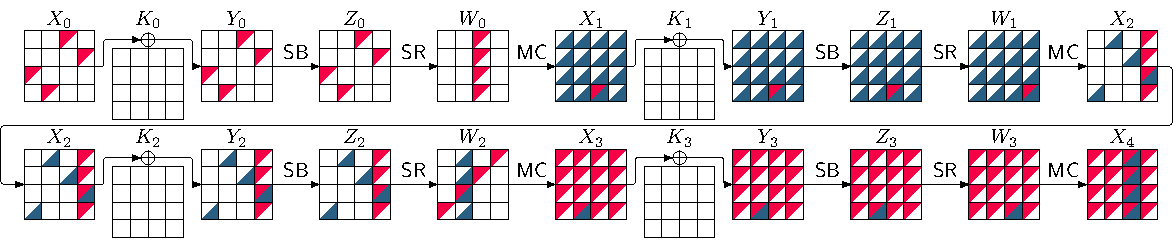
\includegraphics[width=\textwidth]{./figures/aes_sk_4r_v0.pdf} % Replace with your third shape
\end{center}
\begin{center}
  \resizebox{0.9\textwidth}{!}{
\begin{tabular}{@{}cc@{}}
  \toprule
  \multicolumn{2}{c}{$r\Up = 1, r\Mid = 3, r\Low = 0, ~ p = 2^{-24.00}, ~ r = 2^{-7.66}, q^{2} = 1, ~ prq^{2} = \bf 2^{-31.66}$}\\
  \midrule
  $\Delta X_{0}$ \small\texttt{00005200000000f58f000000007b0000} & $\Delta X_{1}$ \small\texttt{0000000000000000000000000000b400}\\
  $\Gamma X_{4}$ \small\texttt{0032000000ab00000066000000980000} & -\\
  \bottomrule
\end{tabular}}
\[{\bf 2^{63.32}}~ \text{v.s.}~2^{150}\]
\end{center}
\end{frame}

%%%%%%%%%%%%%%%%%%%%%%%%%%%%%%%%%%%%%%%%%%%%%%%%%%%%%%%%%%%%%%%%%%%%%%%%
%%%%%%%%%%%%%%%%%%%%%%%%%%%%%%%%%%%%%%%%%%%%%%%%%%%%%%%%%%%%%%%%%%%%%%%%
\section{Boomerang Analysis}
\sectionheader[\huge\color{tug}\faBook]{Boomerang Analysis}

% %%%%%%%%%%%%%%%%%%%%%%%%%%%%%%%%%%%%%%%%%%%%%%%%%%%%%%%%%%%%%%%%%%%%%%%%
% \begin{frame}{Difference Distribution Table (\ddt) -- I}
%   We need a metric to measure the quality of a differential characteristic
%   % \begin{itemize}
%   %   \item compute all possible output differences for all input differences of an
%   %     S-box  
%   % \end{itemize}
%   % \vspace{-0.5cm}
%   \begin{block}{Differential Distribution Table (\ddt)}
%     For a vectorial Boolean function $S: \mathbb{F}_{2}^{n} \rightarrow \mathbb{F}_{2}^{m}$,
%     the \ddt is a $2^{n}\times 2^{m}$ table whose rows correspond to the input difference $\Delta\In$ to $S$ and whose columns correspond to the output difference $\Delta\Out$ of $S$.
%     The entry at index $(\Delta\In, \Delta\Out)$ is
%       \[\ddt(\Delta\In, \Delta\Out) = |\{x\in \mathbb{F}_{2}^{n}:~ S(x) \oplus S(x \oplus \Delta\In) = \Delta\Out\}|.\]
%   \end{block}
%   $\pr\left(\Delta\In,\Delta\Out\right) = 2^{-n}\cdot \ddt\left(\Delta\In,, \Delta\Out\right)$
% \end{frame}

% %%%%%%%%%%%%%%%%%%%%%%%%%%%%%%%%%%%%%%%%%%%%%%%%%%%%%%%%%%%%%%%%%%%%%%%%
% \begin{frame}{Difference Distribution Table (\ddt) -- II}
%   \vspace{-0.3cm}
%   \begin{columns}
%   \column[c]{0.25\textwidth}
%   \begin{center}
%     % \raisebox{-3cm}{%
%     \begin{tikzpicture}
%       \draw (0,0) node[box, name=S, minimum size=2cm] {$\mathcal{S}$};
%       \foreach \i/\a in {1/123,2/101,3/78,4/56} {
%         \draw (S.\a) node[above=2ex] (x\i) {$x_{\i}$};
%         \draw (x\i|-S.south) node[below=2ex] (y\i) {$y_{\i}$};
%         \draw[next] (x\i) -- (x\i|-S.north);
%         \draw[next] (y\i|-S.south) -- (y\i);
%       }

%       \draw (y3) node[tug] {$y_3$};
%       \draw (x1) node[tug] {$x_1$};
%       \draw (x4) node[tug] {$x_4$};

%       \draw[] (x1.south-|S.west) rectangle (x4.north-|S.east);
%       \draw[] (y1.south-|S.west) rectangle (y4.north-|S.east);

%       \foreach \i/\dir in {x1/above, x4/above, y3/below} {\draw (\i) node[\dir=2.5ex, tug] (m\i) {1};}
%       \foreach \i/\dir in {x2/above, x3/above, y1/below, y2/below, y4/below} {\draw (\i) node[\dir=2.5ex] (m\i) {0};}

%       \draw[thick] (mx1.south-|S.west) rectangle (mx4.north-|S.east);
%       \draw[thick] (my1.south-|S.west) rectangle (my4.north-|S.east);

%       \draw (mx4) node[right=3ex] (alpha) {$\Delta\In$};
%       \draw (x4-|alpha) node              {$x$};
%       \draw (y4-|alpha) node              {$\mathcal{S}(x)$};
%       \draw (my4-|alpha) node             {$\Delta\Out$};
      
%     \end{tikzpicture}
%     % }
%   \end{center}
%   \column[c]{0.15\textwidth}  
%   $$\pr\left(\texttt{9}, \texttt{2}\right) = \frac{4}{16}$$
%   \column[c]{0.60\textwidth}
%   \begin{center}
%     \scalebox{0.60}{      
%       \newcommand{\es}{}
%       \begin{tabular}{@{}c|*{3}c*{13}{c}@{}}
%         \toprule
%         $\Delta\In$\,\textbackslash\,$\Delta\Out$ & \es\texttt{0}\es & \es\texttt{1}\es & \es\texttt{2}\es & \es\texttt{3}\es & \es\texttt{4}\es & \es\texttt{5}\es & \es\texttt{6}\es & \es\texttt{7}\es & \es\texttt{8}\es & \es\texttt{9}\es & \es\texttt{a}\es & \es\texttt{b}\es & \es\texttt{c}\es & \es\texttt{d}\es & \es\texttt{e}\es & \es\texttt{f}\es \\
%         \midrule
%         \texttt{0\,} & 16 & 0 & 0 & 0 & 0 & 0 & 0 & 0 & 0 & 0 & 0 & 0 & 0 & 0 & 0 & 0\\
%         \texttt{1\,} & 0 & 0 & 0 & 0 & 2 & 2 & 2 & 2 & 0 & 0 & 0 & 0 & 2 & 2 & 2 & 2\\
%         \texttt{2\,} & 0 & 2 & 0 & 2 & 0 & 0 & 0 & 4 & 0 & 2 & 2 & 0 & 0 & 0 & 2 & 2\\
%         \texttt{3\,} & 0 & 2 & 0 & 2 & 0 & 0 & 4 & 0 & 0 & 2 & 2 & 0 & 0 & 0 & 2 & 2\\
%         \texttt{4\,} & 0 & 0 & 0 & 0 & 0 & 0 & 0 & 0 & 0 & 0 & 4 & 4 & 2 & 2 & 2 & 2\\
%         \texttt{5\,} & 0 & 0 & 0 & 0 & 2 & 2 & 2 & 2 & 0 & 0 & 4 & 4 & 0 & 0 & 0 & 0\\
%         \texttt{6\,} & 0 & 2 & 0 & 2 & 0 & 4 & 0 & 0 & 0 & 2 & 2 & 0 & 2 & 2 & 0 & 0\\
%         \texttt{7\,} & 0 & 2 & 0 & 2 & 4 & 0 & 0 & 0 & 0 & 2 & 2 & 0 & 2 & 2 & 0 & 0\\
%         \texttt{8\,} & 0 & 0 & 0 & 0 & 0 & 0 & 0 & 0 & 0 & 0 & 0 & 0 & 4 & 4 & 4 & 4\\
%         \texttt{9\,} & 0 & 4 & \textcolor{red}{\textbf{4}} & 0 & 0 & 0 & 0 & 0 & 0 & 4 & 0 & 4 & 0 & 0 & 0 & 0\\
%         \texttt{a\,} & 0 & 0 & 2 & 2 & 2 & 0 & 0 & 2 & 4 & 0 & 0 & 0 & 0 & 2 & 0 & 2\\
%         \texttt{b\,} & 0 & 0 & 2 & 2 & 0 & 2 & 2 & 0 & 4 & 0 & 0 & 0 & 2 & 0 & 2 & 0\\
%         \texttt{c\,} & 0 & 4 & 4 & 0 & 2 & 2 & 2 & 2 & 0 & 0 & 0 & 0 & 0 & 0 & 0 & 0\\
%         \texttt{d\,} & 0 & 0 & 0 & 0 & 2 & 2 & 2 & 2 & 0 & 4 & 0 & 4 & 0 & 0 & 0 & 0\\
%         \texttt{e\,} & 0 & 0 & 2 & 2 & 0 & 2 & 2 & 0 & 4 & 0 & 0 & 0 & 0 & 2 & 0 & 2\\
%         \texttt{f\,} & 0 & 0 & 2 & 2 & 2 & 0 & 0 & 2 & 4 & 0 & 0 & 0 & 2 & 0 & 2 & 0\\
%         \bottomrule
%       \end{tabular}
%     }
%   \end{center}
% \end{columns}
% \end{frame}

% %%%%%%%%%%%%%%%%%%%%%%%%%%%%%%%%%%%%%%%%%%%%%%%%%%%%%%%%%%%%%%%%%%%%%%%%
% \begin{frame}{Linear Analysis \cite{eurocrypt_Matsui93}}
%   \vspace{-10pt}
%   \begin{columns}[onlytextwidth]
%     \column[c]{0.3\textwidth}
%     \scalebox{0.65}{
%       \begin{tikzpicture}[scale=0.5]
%         \foreach \i in {0,1,2,3}
%         \draw (0,-\i*4) rectangle ++(6,-2);
%         \foreach \i in {1,2,3}
%         \node[right] at (6,-\i*4+3) {$p_\i$};
%         \foreach \i in {0,1,2,3,4} {
%           \draw[->] (3,-\i*4+2) -- ++(0,-0.75);
%           \draw[<-] (3,-\i*4) -- ++(0,0.75);
%           \draw[<-] (3-0.25,-\i*4+1) -- ++(-1.25,0);
%           \node[left] at (1.5,-\i*4+1) {$K_\i$};          
%           \node[xor] at (3, -\i*4+1) {};
%         }
%         \node[right] at (4,1) {$\lambda_0$};
%         \node[right] at (4,-3) {$\lambda_1$};
%         \node[right] at (4,-7) {$\lambda_2$};
%         \node[right] at (4,-11) {$\lambda_3$};
%         \node[right] at (4,-15) {$\lambda_4$};
%         \draw (3, 2) node[above] {$P$};
%         \draw (3.1, -11) node[right] {$\textcolor{red}{\textbf{Y}}$};
%         \draw (3, -16) node[below] {$C$};
%         % \draw[->,very thick,tug] (6,1) -- ++(0,-12);
%         \path[->,tug,very thick,>=stealth] (6.5,1) edge[bend left]
%           node[rotate=270,above] {$Pr(\lambda\In\cdot P \oplus \lambda\Out \cdot C = 0)$} ++(0,-12);
%         \path[->,blue,very thick,>=stealth] (6.5,-15) edge[bend right] 
%           node[font=\small,rotate=270,above] {guess $K_4$} ++(0,4);
%       \end{tikzpicture}
%     }
%     \column[c]{0.7\textwidth}    
%     \begin{enumerate}
%       \small
%       \item Approximate part of the encryption by a linear function
%         \[
%           \lambda_0\cdot P \oplus \lambda_3\cdot \textcolor{red}{Y} = 0
%         \]
%       \item Guess final key $K_4'$ and determine $\lambda_0\cdot P \oplus \lambda_3 \cdot Y$
%         \medskip
%       \item The right key satisfies $\lambda_0\cdot P \oplus \lambda_3 \cdot Y = 0$, with probability $p = \pr\left(\lambda_0\cdot P \oplus \lambda_3 \cdot Y = 0\right)$ 
%       whereas a wrong key satisfies it with probability $2^{-1}$. 
%         \medskip
%       \item \textit{Necessary condition} for the attack: $\corr \gg 2^{-2n}$, where $\corr = 2\cdot \pr\left(\lambda_0\cdot P \oplus \lambda_3\cdot Y = 0\right) - 1$
%         %, the attack will be faster than exhaustive key search
%     \end{enumerate}
%   \end{columns}
% \end{frame}

% %%%%%%%%%%%%%%%%%%%%%%%%%%%%%%%%%%%%%%%%%%%%%%%%%%%%%%%%%%%%%%%%%%%%%%%%
% \begin{frame}{Linear Approximation Table (\lat) -- I}
%   We need a metric to measure the quality of a linear approximation.
%   \begin{block}{Linear Approximation Table (\lat)}
%     For a vectorial Boolean function $S: \mathbb{F}_{2}^{n} \rightarrow \mathbb{F}_{2}^{m}$, the \lat of $S$ is a $2^{n}\times 2^{m}$ table whose rows correspond to the input mask $\lambda\In$ to $S$ and whose columns correspond to the output mask $\lambda\Out$ of $S$.
%     The entry at index $(\lambda\In, \lambda\Out)$ is
%     \begin{equation*}
%     \lat(\lambda\In, \lambda\Out) = | \lat_0(\lambda\In, \lambda\Out) | - | \lat_1(\lambda\In, \lambda\Out) |,
%     \end{equation*}
%     where $\lat_b(\lambda\In, \lambda\Out) =\{x \in \mathbb{F}_{2}^{n}:~ \lambda\In\cdot x \oplus \lambda\Out \cdot S(x) = b\}$.
%   \end{block}
%   $\corr\left(\lambda\In, \lambda\Out\right) = 2^{-n}\cdot \lat\left(\lambda\In, \lambda\Out\right)$
% \end{frame}

% %%%%%%%%%%%%%%%%%%%%%%%%%%%%%%%%%%%%%%%%%%%%%%%%%%%%%%%%%%%%%%%%%%%%%%%%
% \begin{frame}{Linear Approximation Table (\lat) -- II}
%   \vspace{-5pt}
%   \begin{columns}
%   \column[c]{0.25\textwidth}
%   \begin{center}
%     \raisebox{-3cm}{%
%     \begin{tikzpicture}
%       \draw (0,0) node[box, name=S, minimum size=2cm] {$\mathcal{S}$};
%       \foreach \i/\a in {1/123,2/101,3/78,4/56} {
%         \draw (S.\a) node[above=2ex] (x\i) {$x_{\i}$};
%         \draw (x\i|-S.south) node[below=2ex] (y\i) {$y_{\i}$};
%         \draw[next] (x\i) -- (x\i|-S.north);
%         \draw[next] (y\i|-S.south) -- (y\i);
%       }

%       \draw (y2) node[tug] {$y_2$};
%       \draw (x1) node[tug] {$x_1$};
%       \draw (x4) node[tug] {$x_4$};

%       \draw[] (x1.south-|S.west) rectangle (x4.north-|S.east);
%       \draw[] (y1.south-|S.west) rectangle (y4.north-|S.east);

%       \foreach \i/\dir in {x1/above, x4/above, y2/below} {\draw (\i) node[\dir=2.5ex, tug] (m\i) {1};}
%       \foreach \i/\dir in {x2/above, x3/above, y1/below, y3/below, y4/below} {\draw (\i) node[\dir=2.5ex] (m\i) {0};}

%       \draw[thick] (mx1.south-|S.west) rectangle (mx4.north-|S.east);
%       \draw[thick] (my1.south-|S.west) rectangle (my4.north-|S.east);

%       \draw (mx4) node[right=3ex] (alpha) {$\lambda\In$};
%       \draw (x4-|alpha) node              {$x$};
%       \draw (y4-|alpha) node              {$\mathcal{S}(x)$};
%       \draw (my4-|alpha) node             {$\lambda\Out$};
      
%     \end{tikzpicture}
%     }
%   \end{center}
%   \column[c]{0.15\textwidth}
%   $$\corr\left(\texttt{9}, \texttt{4}\right) = \frac{8}{16}$$
%   \column[c]{0.60\textwidth}
%   \begin{center}
%     \scalebox{0.60}{      
%       \newcommand{\es}{}
%       \begin{tabular}{@{}c|*{3}c*{13}{c}@{}}
%         \toprule
%         $\lambda\In$\,\textbackslash\,$\lambda\Out$ & \es\texttt{0}\es & \es\texttt{1}\es & \es\texttt{2}\es & \es\texttt{3}\es & \es\texttt{4}\es & \es\texttt{5}\es & \es\texttt{6}\es & \es\texttt{7}\es & \es\texttt{8}\es & \es\texttt{9}\es & \es\texttt{a}\es & \es\texttt{b}\es & \es\texttt{c}\es & \es\texttt{d}\es & \es\texttt{e}\es & \es\texttt{f}\es \\
%         \midrule
%         \texttt{0\,} & 16 & 0 & 0 & 0 & 0 & 0 & 0 & 0 & 0 & 0 & 0 & 0 & 0 & 0 & 0 & 0\\
%         \texttt{1\,} & 0 & 0 & 4 & -4 & 0 & -8 & -4 & -4 & 0 & 0 & 4 & -4 & -8 & 0 & 4 & 4\\
%         \texttt{2\,} & 0 & 0 & 0 & 0 & 0 & 0 & 0 & 0 & 0 & 8 & 8 & 0 & 0 & 8 & -8 & 0\\
%         \texttt{3\,} & 0 & -8 & 4 & 4 & 0 & 0 & -4 & 4 & 0 & 0 & -4 & 4 & -8 & 0 & -4 & -4\\
%         \texttt{4\,} & 0 & 4 & 0 & 4 & 0 & 4 & 8 & -4 & 0 & 4 & 0 & 4 & -8 & -4 & 0 & 4\\
%         \texttt{5\,} & 0 & 4 & -4 & -8 & 0 & -4 & -4 & 0 & 0 & 4 & -4 & 8 & 0 & -4 & -4 & 0\\
%         \texttt{6\,} & 0 & -4 & 8 & 4 & 0 & -4 & 0 & -4 & 0 & 4 & 0 & 4 & 8 & -4 & 0 & 4\\
%         \texttt{7\,} & 0 & 4 & 4 & 0 & 0 & -4 & 4 & -8 & 0 & -4 & -4 & 0 & 0 & 4 & -4 & -8\\
%         \texttt{8\,} & 0 & 0 & 0 & 0 & 0 & 0 & 0 & 0 & 0 & 0 & 8 & 8 & 0 & 0 & 8 & -8\\
%         \texttt{9\,} & 0 & 0 & -4 & 4 & \textcolor{red}{\textbf{8}} & 0 & -4 & -4 & 0 & 0 & 4 & -4 & 0 & -8 & -4 & -4\\
%         \texttt{a\,} & 0 & 8 & 0 & 8 & 0 & -8 & 0 & 8 & 0 & 0 & 0 & 0 & 0 & 0 & 0 & 0\\
%         \texttt{b\,} & 0 & 0 & -4 & 4 & -8 & 0 & -4 & -4 & 0 & 8 & -4 & -4 & 0 & 0 & 4 & -4\\
%         \texttt{c\,} & 0 & 4 & 0 & 4 & 0 & 4 & -8 & -4 & 8 & -4 & 0 & 4 & 0 & 4 & 0 & 4\\
%         \texttt{d\,} & 0 & 4 & 4 & 0 & -8 & 4 & -4 & 0 & -8 & -4 & 4 & 0 & 0 & -4 & -4 & 0\\
%         \texttt{e\,} & 0 & 4 & 8 & -4 & 0 & 4 & 0 & 4 & 8 & 4 & 0 & -4 & 0 & -4 & 0 & -4\\
%         \texttt{f\,} & 0 & -4 & -4 & 0 & -8 & -4 & 4 & 0 & 8 & -4 & 4 & 0 & 0 & -4 & -4 & 0\\
%         \bottomrule
%       \end{tabular}
%     }
%   \end{center}
% \end{columns}
% \end{frame}

%%%%%%%%%%%%%%%%%%%%%%%%%%%%%%%%%%%%%%%%%%%%%%%%%%%%%%%%%%%%%%%%%%%%%%%%
\begin{frame}{Boomerang Distinguishers \cite{fse_Wagner99}}
\vspace{-0.55cm}
\begin{columns}
\column[c]{0.4\textwidth}
\centering
\resizebox{1.3\textwidth}{!}{
\begin{tikzpicture}[baseline=1cm, very thick]
\pgfmathsetmacro{\hstep}{0.9};
\pgfmathsetmacro{\vstep}{1.8};
\pgfmathsetmacro{\length}{8*\hstep};
\pgfmathsetmacro{\halflength}{\length/2};
\pgfmathsetmacro{\hight}{1};
\pgfmathsetmacro{\halfhight}{\hight/2};
\node[] (r1) at (0, 0) {$\Delta$};
\node[right=\hstep of r1] (c1) {};
\node[right=\halflength of c1] (c2) {};
\node[right=\halflength of c2] (c3) {};
\node[right=\hstep of c3] (c4) {$\nabla$};
\visible<1->{%
\draw[rounded corners=3pt] ($(c1) + (0, -\halfhight)$) rectangle ($(c3) + (0, \halfhight)$) node[pos=.5] {$E:\mathbb{F}_{2}^{n} \rightarrow \mathbb{F}_{2}^{n}$};
\draw[->] (r1) -- (c1);
\draw[->] (c3) -- (c4);
\visible<1>{%
\node[below=2*\halfhight of c2] (text) {$0 \lneq \pr(\Delta \xrightarrow{E} \nabla) \lll 2^{-n}$};
}}
\visible<2->{%
\draw[rounded corners=3pt, fill=white] ($(c1) + (0, -\halfhight)$) rectangle ($(c3) + (0, \halfhight)$);
\draw[gray] ($(c2) + (0, -\halfhight)$) -- ($(c2) + (0, \halfhight)$);
\node[] at ($0.5*(c1) + 0.5*(c2)$) {$E\Up$};
\node[] at ($0.5*(c2) + 0.5*(c3)$) {$E\Low$};
% Shift the axes down by \vstep units
\node[below=\vstep of r1] (r1) {$\Delta_{1}$};
\node[right=\hstep of r1] (c1) {};
\node[right=\halflength of c1] (c2) {};
\node[right=\halflength of c2] (c3) {};
\draw[rounded corners=3pt, fill=tugred] ($(c1) + (0, -\halfhight)$) rectangle ($(c2) + (0, \halfhight)$) node[pos=.5] {$E\Up$};
\node[right=\hstep of c2] (temp) {$\Delta_{2}$};
\draw[->] (r1) -- (c1);
\draw[->] (c2) -- (temp);
\node[] at ($0.5*(c1) + 0.5*(c2) + (0, \hstep)$) {$p = \pr(\Delta_{1} \xrightarrow{E\Up} \Delta_{2})$};
% Shift the axes down by \vstep units
\node[below=\vstep of r1] (r1) {};
\node[right=\hstep of r1] (c1) {};
\node[right=\halflength of c1] (c2) {};
\node[right=\halflength of c2] (c3) {};
\draw[rounded corners=3pt, fill=tugblue] ($(c2) + (0, -\halfhight)$) rectangle ($(c3) + (0, \halfhight)$) node[pos=.5] {$\textcolor{white}{E\Low}$};
\node[left=\hstep of c2] (temp1) {$\nabla_{2}$};
\node[right=\hstep of c3] (temp2) {$\nabla_{3}$};
\draw[->] (temp1) -- (c2);
\draw[->] (c3) -- (temp2);
\node[] at ($0.5*(c2) + 0.5*(c3) + (0, \hstep)$) {$q = \pr(\nabla_{2} \xrightarrow{E\Up} \nabla_{3})$};
% Shift the axes down by \halfhight+0.2 units
\node[below=\halfhight+0.2 of r1] (r1) {};
\node[right=\hstep of r1] (c1) {};
\node[right=\halflength of c1] (c2) {};
\visible<6>{
\node[fill=tugyellow, below=0.5 of c2] (pnode) {{\large$\textcolor{black}{\pr(P_{3} \oplus P_{4} = \Delta_{1}) = p^{2} q^{2}}$}};
}
% \node[fill=tugyellow] at (c2) {$p^{2}q^{2} \ggg 2^{-n}$};
}
\end{tikzpicture}}
\column[c]{0.6\textwidth}
\begin{flushright}
\resizebox*{0.7\textwidth}{!}{
\begin{tikzpicture}[yscale=1,xscale=1, baseline=-1cm, thick]
\pgfmathsetmacro{\deltai}{3.3};
\pgfmathsetmacro{\nablao}{3.5};
\pgfmathsetmacro{\depth}{6};
\pgfmathsetmacro{\halfdepth}{\depth/2};
\pgfmathsetmacro{\quarterfdepth}{\depth/4};
\pgfmathsetmacro{\verticaldownshift}{1};
\visible<3->{%
\node (p1) at (0, 0) {$P_{1}$};
\node (p2) at ($(p1) + (\deltai, -\verticaldownshift)$) {$P_{2}$};
\node[below=\halfdepth of p1] (x1) {$X_{1}$};
\node[below=\halfdepth of p2] (x2) {$X_{2}$};
\node[box, below=\quarterfdepth of p1.center, fill=tugred] (e0l1) {$E\Up$};
\node[box, below=\quarterfdepth of p2.center, fill=tugred] (e0l2) {$E\Up$};
\node[below=\halfdepth of x1] (c1) {$C_{1}$};
\node[below=\halfdepth of x2] (c2) {$C_{2}$};
\node[box, below=\quarterfdepth of x1.center, fill=tugblue] (e1l1) {$\textcolor{white}{E\Low}$};
\node[box, below=\quarterfdepth of x2.center, fill=tugblue] (e1l2) {$\textcolor{white}{E\Low}$};
\draw[<->, dashed, red] (p1) -- node[above] {$\Delta_{1}$} (p2);
\draw[<->, dashed, red] (x1) -- node[below] {$\Delta_{2}$} (x2);
\draw[->] (p1) -- (e0l1) -- (x1);
\draw[->] (x1) -- (e1l1) -- (c1);
\draw[->] (p2) -- (e0l2) -- (x2);
\draw[->] (x2) -- (e1l2) -- (c2);
\node[right=\nablao of c1] (c3) {\textcolor{white}{$C_{3}$}};
\node[right=\nablao of c2] (c4) {\textcolor{white}{$C_{4}$}};
}

\visible<4->{%
\node[right=\nablao of c1] (c3) {$C_{3}$};
\node[right=\nablao of c2] (c4) {$C_{4}$};
\draw[<->, dashed, blue] (c1) -- node[above] {$\nabla_{3}$} (c3);
\draw[<->, dashed, blue] (c2) -- node[above] {$\nabla_{3}$} (c4);
}

\visible<5->{%
\node[right=\nablao of x1] (x3) {$X_{3}$};
\node[right=\nablao of x2] (x4) {$X_{4}$};
\node[box, below=\quarterfdepth of x3.center, fill=tugblue] (e1r1) {$\textcolor{white}{E\Low}$};
\node[box, below=\quarterfdepth of x4.center, fill=tugblue] (e1r2) {$\textcolor{white}{E\Low}$};
\draw[<->, dashed, blue] (x1) -- node[above] {$\nabla_{2}$} (x3);
\draw[<->, dashed, blue] (x2) -- node[below] {$\nabla_{2}$} (x4);
\draw[->] (c3) -- (e1r1) -- (x3);
\draw[->] (c4) -- (e1r2) -- (x4);
}
\visible<6>{
\node[right=\nablao of p1] (p3) {$P_{3}$};
\node[right=\nablao of p2] (p4) {$P_{4}$};
\node[box, below=\quarterfdepth of p3.center, fill=tugred] (e0r1) {$E\Up$};
\node[box, below=\quarterfdepth of p4.center, fill=tugred] (e0r2) {$E\Up$};
\draw[->] (x3) -- (e0r1) -- (p3);
\draw[->] (x4) -- (e0r2) -- (p4);

\draw[<->, dashed, red] (x3) -- node[above] {$\Delta_{2}$} (x4);
\draw[<->, dashed, red] (p3) -- node[above] {$\Delta_{1}$} (p4);
}
\end{tikzpicture}}
\end{flushright}
\end{columns}
\end{frame}

%%%%%%%%%%%%%%%%%%%%%%%%%%%%%%%%%%%%%%%%%%%%%%%%%%%%%%%%%%%%%%%%%%%%%%%%
\begin{frame}{Sandwiching the Differentials! \cite{conf_crypto_DunkelmanKS10, joc_DunkelmanKS14}}
% \vspace{-0.4cm}
\begin{columns}
\column[c]{0.5\textwidth}
\centering
\only<1->{%
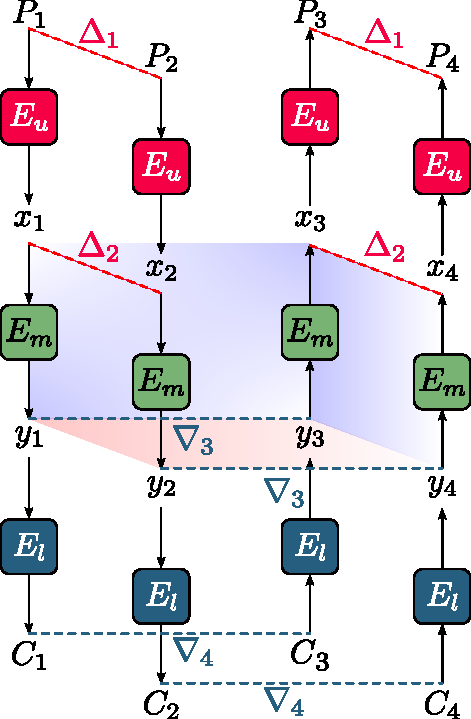
\includegraphics[width=0.55\textwidth]{./figures/sandwich.pdf}
}
\column[c]{0.5\textwidth}
\centering
\only<1>{%

\includegraphics[width=0.65\textwidth]{./figures/realsandwich.pdf}
}
\only<2>{%
\begin{gather*}
\pr(P_{3} \oplus P_{4} = \textcolor{red}{\Delta_{1}}) \approx p^{2}\times r \times q^{2}\\
r = \pr(\textcolor{red}{\Delta_{2}} \rightleftarrows \textcolor{blue}{\nabla_{3}})
\end{gather*}
}
\end{columns}
% \only<3>{%
% {\small
% \[\pr\left(P_{3} \oplus P_{4} = \Delta_{1}\right) = \sum_{\Delta_{2}, \Delta_{2}', \nabla_{3}, \nabla_{3}'} p_{\nabla{3}}\times p_{\nabla_{3}'} \times r(\Delta_{2}, \Delta_{2}', \nabla_{3}, \nabla_{3}') \times q_{\nabla_{3}} \times q_{\nabla_{3}'}\]
% }
% }
\end{frame}

%%%%%%%%%%%%%%%%%%%%%%%%%%%%%%%%%%%%%%%%%%%%%%%%%%%%%%%%%%%%%%%%%%%%%%%%
\begin{frame}{Boomerang Connectivity Table (BCT) \cite{eurocrypt_CidHPSS18}}
\begin{columns}
\column[c]{0.5\textwidth}
\centering
\resizebox{0.8\textwidth}{!}{
\begin{tikzpicture}[yscale=0.6,xscale=1, baseline=-1cm, thin]
  \pgfmathsetmacro{\deltai}{2.6};
  \pgfmathsetmacro{\nablao}{2.8};
  \pgfmathsetmacro{\depth}{5};
  \pgfmathsetmacro{\halfdepth}{\depth/2};
  \pgfmathsetmacro{\quarterfdepth}{\depth/4};
  \pgfmathsetmacro{\verticaldownshift}{1.2};
  \node (x1) at (0, 0) {$X_{1}$};
  \node (x2) at ($(x1) + (\deltai, -\verticaldownshift)$) {$X_{2}$};
  \node[below=\halfdepth of x1] (y1) {$Y_{1}$};
  \node[below=\halfdepth of x2] (y2) {$Y_{2}$};
  \node[box, below=\quarterfdepth of x1.center, fill=tuggreen] (e1l1) {$S$};
  \node[box, below=\quarterfdepth of x2.center, fill=tuggreen] (e1l2) {$S$};
  \draw[<->, dashed, red] (x1) -- node[above] {$\Delta_{1}$} (x2);
  \draw[->] (x1) -- (e1l1) -- (y1);
  \draw[->] (x2) -- (e1l2) -- (y2);
  \node[right=\nablao of y1] (y3) {$Y_{3}$};
  \node[right=\nablao of y2] (y4) {$Y_{4}$};
  \draw[<->, dashed, blue] (y1) -- node[above] {$\nabla_{2}$} (y3);
  \draw[<->, dashed, blue] (y2) -- node[above] {$\nabla_{2}$} (y4);
  \node[right=\nablao of x1] (x3) {$X_{3}$};
  \node[right=\nablao of x2] (x4) {$X_{4}$};
  \node[box, below=\quarterfdepth of x3.center, fill=tuggreen] (e1r1) {$S^{-1}$};
  \node[box, below=\quarterfdepth of x4.center, fill=tuggreen] (e1r2) {$S^{-1}$};
  \draw[->] (y3) -- (e1r1) -- (x3);
  \draw[->] (y4) -- (e1r2) -- (x4);
  \draw[<->, red, dashed] (x3) -- node[above] {$\textcolor{red}{\Delta_{1}}$} (x4);
\end{tikzpicture}
}
\column[c]{0.5\textwidth}
\centering
\begin{tikzpicture}
  \pgfmathsetmacro{\lth}{4};
  \pgfmathsetmacro{\htt}{2};
  \node[upper] (D1) at (0, 0) {$\Delta_{1}$};
  \node[right=\lth of D1, gray] (D2) {$\Delta_{2}$};
  \node[below=\htt of D1, gray] (L1) {$\nabla_{1}$};
  \node[right=\lth of L1, lower] (L2) {$\nabla_{2}$};
  \draw[->, very thick, gray] (D1) -- node[above]{$\ddt$} (D2);
  \draw[->, very thick] (D1) -- node[above] {$\bct$} (L2);
  \draw[<-, very thick, gray] (L1) -- node[below] {$\ddt$} (L2);
\end{tikzpicture}
\end{columns}
\vspace{0.2cm}
\only<1->{
{\small
\[\texttt{BCT}(\textcolor{red}{\Delta_{1}}, \textcolor{blue}{\nabla_{2}}) \coloneqq \#\{X\in \mathbb{F}_{2}^{n}\,|\,S^{-1}\left(S(X) \oplus \textcolor{blue}{\nabla_{2}}\right) \oplus S^{-1}(S(X \oplus \textcolor{red}{\Delta_{1}}) \oplus \textcolor{blue}{\nabla_{2}}) = \textcolor{red}{\Delta_{1}}\}\]
}
}
\onslide<1->{
{\small
% \[\texttt{BCT}(\textcolor{red}{0}, \textcolor{blue}{\nabla}) = \texttt{BCT}(\textcolor{red}{\Delta}, \textcolor{blue}{0}) = 2^{n}\]
\[\pr(\Delta_{1} \rightleftarrows \nabla_{2}) = 2^{-n}\cdot\bct(\textcolor{red}{\Delta_{1}}, \textcolor{blue}{\nabla_{2}})\]
}
}
\end{frame}

%%%%%%%%%%%%%%%%%%%%%%%%%%%%%%%%%%%%%%%%%%%%%%%%%%%%%%%%%%%%%%%%%%%%%%%%
\begin{frame}{Generalized BCT Framework (GBCT) - I}
\vspace{-0.4cm}
\begin{columns}
\column[c]{0.5\textwidth}
\begin{center}
\resizebox{0.5\textwidth}{!}{
\begin{tikzpicture}[yscale=0.6,xscale=1, baseline=-1cm, thin]
  \pgfmathsetmacro{\deltai}{2.6};
  \pgfmathsetmacro{\nablao}{2.8};
  \pgfmathsetmacro{\depth}{5};
  \pgfmathsetmacro{\halfdepth}{\depth/2};
  \pgfmathsetmacro{\quarterfdepth}{\depth/4};
  \pgfmathsetmacro{\verticaldownshift}{1.2};
  \node (x1) at (0, 0) {$X_{1}$};
  \node (x2) at ($(x1) + (\deltai, -\verticaldownshift)$) {$X_{2}$};
  \node[below=\halfdepth of x1] (y1) {$Y_{1}$};
  \node[below=\halfdepth of x2] (y2) {$Y_{2}$};
  \node[box, below=\quarterfdepth of x1.center, fill=tuggreen] (e1l1) {$S$};
  \node[box, below=\quarterfdepth of x2.center, fill=tuggreen] (e1l2) {$S$};
  \draw[<->, dashed, red] (x1) -- node[above] {$\Delta_{1}$} (x2);
  \draw[->] (x1) -- (e1l1) -- (y1);
  \draw[->] (x2) -- (e1l2) -- (y2);
  \node[right=\nablao of y1] (y3) {$Y_{3}$};
  \node[right=\nablao of y2] (y4) {$Y_{4}$};
  \draw[<->, dashed, blue] (y1) -- node[above] {$\nabla_{2}$} (y3);
  \draw[<->, dashed, blue] (y2) -- node[above] {$\nabla_{2}$} (y4);
  \node[right=\nablao of x1] (x3) {$X_{3}$};
  \node[right=\nablao of x2] (x4) {$X_{4}$};
  \node[box, below=\quarterfdepth of x3.center, fill=tuggreen] (e1r1) {$S^{-1}$};
  \node[box, below=\quarterfdepth of x4.center, fill=tuggreen] (e1r2) {$S^{-1}$};
  \draw[->] (y3) -- (e1r1) -- (x3);
  \draw[->] (y4) -- (e1r2) -- (x4);
  \draw[<->, red, dashed] (x3) -- node[above] {$\textcolor{red}{\Delta_{1}}$} (x4);
\end{tikzpicture}}
\end{center}
~~~~~~~~~~~~~~
\column[c]{0.5\textwidth}
\centering
\begin{tikzpicture}
\pgfmathsetmacro{\lth}{2};
\pgfmathsetmacro{\htt}{1};
\only<1>{
	\node[red] (d1) at (0, 0) {$\Delta_{1}$};
	\node[right=\lth of d1, red] (d2) {$\Delta_{2}$};
	\node[below=\htt of d1, blue] (n1) {$\nabla_{1}$};
	\node[right=\lth of n1, blue] (n2) {$\nabla_{2}$};
}
\only<1>{
	\node[red] (d1) at (0, 0) {$\Delta_{1}$};
	\node[right=\lth of d1, red] (d2) {$\Delta_{2}$};
	\node[below=\htt of d1, blue] (n1) {$\nabla_{1}$};
	\node[right=\lth of n1, blue] (n2) {$\nabla_{2}$};
	\draw[->] (d1) -- (d2);
	\draw[<-] (n1) -- (n2);
}
\only<2>{
	\node[red] (d1) at (0, 0) {$\Delta_{1}$};
	\node[right=\lth of d1, gray] (d2) {$\Delta_{2}$};
	\node[below=\htt of d1, gray] (n1) {$\nabla_{1}$};
	\node[right=\lth of n1, blue] (n2) {$\nabla_{2}$};
	\draw[->] (d1) -- (n2);
}
\only<3>{
	\node[red] (d1) at (0, 0) {$\Delta_{1}$};
	\node[right=\lth of d1, red] (d2) {$\Delta_{2}$};
	\node[below=\htt of d1, gray] (n1) {$\nabla_{1}$};
	\node[right=\lth of n1, blue] (n2) {$\nabla_{2}$};
	\draw[->] (d1) -- (d2);
	\draw[->] (d1) -- (n2);
}
\only<4>{
	\node[red] (d1) at (0, 0) {$\Delta_{1}$};
	\node[right=\lth of d1, gray] (d2) {$\Delta_{2}$};
	\node[below=\htt of d1, blue] (n1) {$\nabla_{1}$};
	\node[right=\lth of n1, blue] (n2) {$\nabla_{2}$};
	\draw[->] (d1) -- (n2);
	\draw[<-] (n1) -- (n2);
}
\only<5>{
	\node[red] (d1) at (0, 0) {$\Delta_{1}$};
	\node[right=\lth of d1, red] (d2) {$\Delta_{2}$};
	\node[below=\htt of d1, blue] (n1) {$\nabla_{1}$};
	\node[right=\lth of n1, blue] (n2) {$\nabla_{2}$};
	\draw[->] (d1) -- (d2);
	\draw[->] (d1) -- (n2);
	\draw[<-] (n1) -- (n2);
}
\end{tikzpicture}
\end{columns}
\vspace{-0.4cm}
\begin{itemize}
\item<1->[\faCheckCircle]{\scriptsize $\mathcal{X}_{\ddt}(\Delta_{1}, \Delta_{2}) = \{x: S(x) \oplus S(x \oplus \Delta_{1}) = \Delta_{2}\}, \quad \texttt{DDT}(\Delta_{1}, \Delta_{2}) = \# \mathcal{X}_{\ddt}(\Delta_{1}, \Delta_{2})$}
\item<2->[\faCheckCircle]{\scriptsize $\mathcal{X}_{\bct}(\Delta_{1}, \nabla_{2}) = \{x: S^{-1}(S(x) \oplus \nabla_{2}) \oplus S^{-1}(S(x \oplus \Delta_{1}) \oplus \nabla_{2}) = \Delta_{1}\}, ~ \texttt{BCT}(\Delta_{1}, \nabla_{2}) = \# \mathcal{X}_{\bct}(\Delta_{1}, \nabla_{2})$ \hspace*{\fill}}
\item<3->[\faCheckCircle]{\scriptsize $\ubct(\Delta_{1}, \Delta_{2}, \nabla_{2}) = \# \{x: x\in \mathcal{X}_{\texttt{BCT}}(\Delta_{1}, \nabla_{2}) \cap \mathcal{X}_{\texttt{DDT}}(\Delta_{1}, \Delta_{2})\}$ \hspace*{\fill} \cite{tosc_WangP19}}
\item<4->[\faCheckCircle]{\scriptsize $\lbct(\Delta_{1}, \nabla_{1}, \nabla_{2}) = \#\{x: x \in \mathcal{X}_{\texttt{BCT}}(\Delta_{1}, \nabla_{2}) \cap \mathcal{X}_{\texttt{DDT}}(\nabla_{1}, \nabla_{2})\}$ \hspace*{\fill} \cite{tosc_DelauneDV20, tosc_SongQH19}}
\item<5->[\faCheckCircle]{\scriptsize $\ebct(\Delta_{1}, \Delta_{2}, \nabla_{1}, \nabla_{2}) = \#\{x: x\in \mathcal{X}_{\texttt{BCT}}(\Delta_{1}, \nabla_{2}) \cap \mathcal{X}_{\texttt{DDT}}(\Delta_{1}, \Delta_{2}) \cap \mathcal{X}_{\texttt{DDT}}(\nabla_{1}, \nabla_{2})\}$ \hspace*{\fill} \cite{tosc_BoukerrouHLMM20, tosc_DelauneDV20}}
\end{itemize}
\end{frame}

%%%%%%%%%%%%%%%%%%%%%%%%%%%%%%%%%%%%%%%%%%%%%%%%%%%%%%%%%%%%%%%%%%%%%%%%
\begin{frame}{Generalized BCT Framework (GBCT) - II}
\vspace{-0.4cm}
\begin{itemize}
  \item Double Boomerang Connectivity Table (\texttt{DBCT}) \cite{tosc_HadipourBS21}
\end{itemize}
\begin{columns}
\column[c]{0.7\textwidth}
\begin{figure}
\centering
\begin{tikzpicture}
\pgfmathsetmacro{\lth}{2};
\pgfmathsetmacro{\htt}{0.6};
	\node[red] (d1) at (0, 0) {$\Delta_{1}$};
	\node[red] at ($(d1) + (\lth, 0)$) (d2) {\only<1>{$\Delta_{2}$}\only<2->{$\Delta_{2}^{\bf{*}}$}};
	\node[blue] at ($(d1) + (\lth, -2*\htt)$) (n1) {\only<1>{$\nabla_{2}^{\bf{*}}$}\only<2>{$\nabla_{2}$}\only<3>{$\nabla_{2}^{\bf{*}}$}};
	\node[blue] at ($(n1) + (\lth, 0)$) (n2) {$\nabla_{3}$};
	\draw[->] (d1) -- (d2);
	\draw[->] (n1) -- (n2);
	\draw[->] (d1) -- (n1);
	\draw[->] (d2) -- (n2);
\end{tikzpicture}
\end{figure}
\begin{itemize}
\vspace{-0.4cm}
\item<1->[\faCheckCircleO] {\scriptsize $\texttt{DBCT}^{\vdash}(\Delta_{1}, \Delta_{2}, \nabla_{3}) = \sum_{\nabla_{2}} \ubct(\Delta_{1}, \Delta_{2}, \nabla_{2})\cdot \lbct(\Delta_{2}, \nabla_{2}, \nabla_{3})$}
\item<2->[\faCheckCircleO] {\scriptsize $\texttt{DBCT}^{\dashv}(\Delta_{1}, \nabla_{2}, \nabla_{3}) = \sum_{\Delta_{2}} \ubct(\Delta_{1}, \Delta_{2}, \nabla_{2})\cdot \lbct(\Delta_{2}, \nabla_{2}, \nabla_{3}).$}
\item<3->[\faCheckCircleO] {\scriptsize $\texttt{DBCT}(\Delta_{1}, \nabla_{3}) = \sum_{\Delta_{2}}\dbct^{\vdash}(\Delta_{1}, \Delta_{2}, \nabla_{3}) = \sum_{\nabla_{2}}\dbct^{\dashv}(\Delta_{1}, \nabla_{2}, \nabla_{3}).$}
\end{itemize}
\column[c]{0.3\textwidth}
\vspace{-0.4cm}
\begin{figure}
\centering
\resizebox{0.96\textwidth}{!}{
\begin{tikzpicture}[yscale=0.6,xscale=1, baseline=-1cm]
  \pgfmathsetmacro{\deltai}{2.7};
  \pgfmathsetmacro{\nablao}{3};
  \pgfmathsetmacro{\depth}{5.5};
  \pgfmathsetmacro{\halfdepth}{\depth/2};
  \pgfmathsetmacro{\quarterfdepth}{\depth/4};
  \pgfmathsetmacro{\verticaldownshift}{1.2};
  \node (x1) at (0, 0) {$X_{1}$};
  \node (x2) at ($(x1) + (\deltai, -\verticaldownshift)$) {$X_{2}$};
  \node[below=\halfdepth of x1] (y1) {$Y_{1}$};
  \node[below=\halfdepth of x2] (y2) {$Y_{2}$};
  \node[box, below=\quarterfdepth of x1.center, fill=tuggreen] (e1l1) {$S$};
  \node[box, below=\quarterfdepth of x2.center, fill=tuggreen] (e1l2) {$S$};
  \draw[<->, dashed, red] (x1) -- node[above] {$\Delta_{1}$} (x2);
  \draw[->] (x1) -- (e1l1) -- (y1);
  \draw[->] (x2) -- (e1l2) -- (y2);
  \node[right=\nablao of y1] (y3) {$Y_{3}$};
  \node[right=\nablao of y2] (y4) {$Y_{4}$};
  \draw[<->, dashed, blue] (y1) -- node[above] {$\nabla_{2}$} (y3);
  \draw[<->, dashed, blue] (y2) -- node[above] {$\nabla_{2}$} (y4);
  \node[right=\nablao of x1] (x3) {$X_{3}$};
  \node[right=\nablao of x2] (x4) {$X_{4}$};
  \node[box, below=\quarterfdepth of x3.center, fill=tuggreen] (e1r1) {$S^{-1}$};
  \node[box, below=\quarterfdepth of x4.center, fill=tuggreen] (e1r2) {$S^{-1}$};
  \draw[->] (y3) -- (e1r1) -- (x3);
  \draw[->] (y4) -- (e1r2) -- (x4);
  \draw[<->, red, dashed] (x3) -- node[above] {$\textcolor{red}{\Delta_{1}}$} (x4);
  
  \node[xor, below=0.5 of y1] (xor1) {};
  \node[xor, below=0.5 of y2] (xor2) {};
  \node[xor, below=0.5 of y3] (xor3) {};
  \node[xor, below=0.5 of y4] (xor4) {};
  \draw[->] (y1) -- (xor1);
  \draw[->]  (xor1)++(-0.5, 0) -- node[left] {$\$$} (xor1);
  \draw[->] (y2) -- (xor2);
  \draw[->]  (xor2)++(-0.5, 0) -- node[left] {$\$$} (xor2);
  \draw[->] (y3) -- (xor3);
  \draw[->]  (xor3)++(0.5, 0) -- node[right] {$\$$} (xor3);
  \draw[->] (y4) -- (xor4);
  \draw[->]  (xor4)++(0.5, 0) -- node[right] {$\$$} (xor4);
  \node[below=1.2cm of y1] (x1) {$Y'_{1}$};
  \node[below=1.2cm of y2] (x2) {$Y'_{2}$};
  \node[below=\halfdepth of x1] (y1) {$Z_{1}$};
  \node[below=\halfdepth of x2] (y2) {$Z_{2}$};
  \node[box, below=\quarterfdepth of x1.center, fill=tuggreen] (e1l1) {$S$};
  \node[box, below=\quarterfdepth of x2.center, fill=tuggreen] (e1l2) {$S$};
  \draw[<->, dashed, red] (x1) -- node[above] {$\Delta_{2}$} (x2);
  \draw[->] (x1) -- (e1l1) -- (y1);
  \draw[->] (x2) -- (e1l2) -- (y2);
  \node[right=\nablao of y1] (y3) {$Z_{3}$};
  \node[right=\nablao of y2] (y4) {$Z_{4}$};
  \draw[<->, dashed, blue] (y1) -- node[above] {$\nabla_{3}$} (y3);
  \draw[<->, dashed, blue] (y2) -- node[above] {$\nabla_{3}$} (y4);
  \node[right=\nablao of x1] (x3) {$Y'_{3}$};
  \node[right=\nablao of x2] (x4) {$Y'_{4}$};
  \draw[->] (xor1) -- (x1);
  \draw[->] (xor2) -- (x2);
  \draw[->] (xor3) -- (x3);
  \draw[->] (xor4) -- (x4);
  \node[box, below=\quarterfdepth of x3.center, fill=tuggreen] (e1r1) {$S^{-1}$};
  \node[box, below=\quarterfdepth of x4.center, fill=tuggreen] (e1r2) {$S^{-1}$};
  \draw[->] (y3) -- (e1r1) -- (x3);
  \draw[->] (y4) -- (e1r2) -- (x4);
  \draw[<->, red, dashed] (x3) -- node[above] {$\textcolor{red}{\Delta_{2}}$} (x4);
\end{tikzpicture}}
\end{figure}
\end{columns}
\end{frame}

%%%%%%%%%%%%%%%%%%%%%%%%%%%%%%%%%%%%%%%%%%%%%%%%%%%%%%%%%%%%%%%%%%%%%%%%
\begin{frame}{Application of GBCT \cite{tosc_HadipourBS21}}
\only<1>{
\begin{figure}
	\centering
	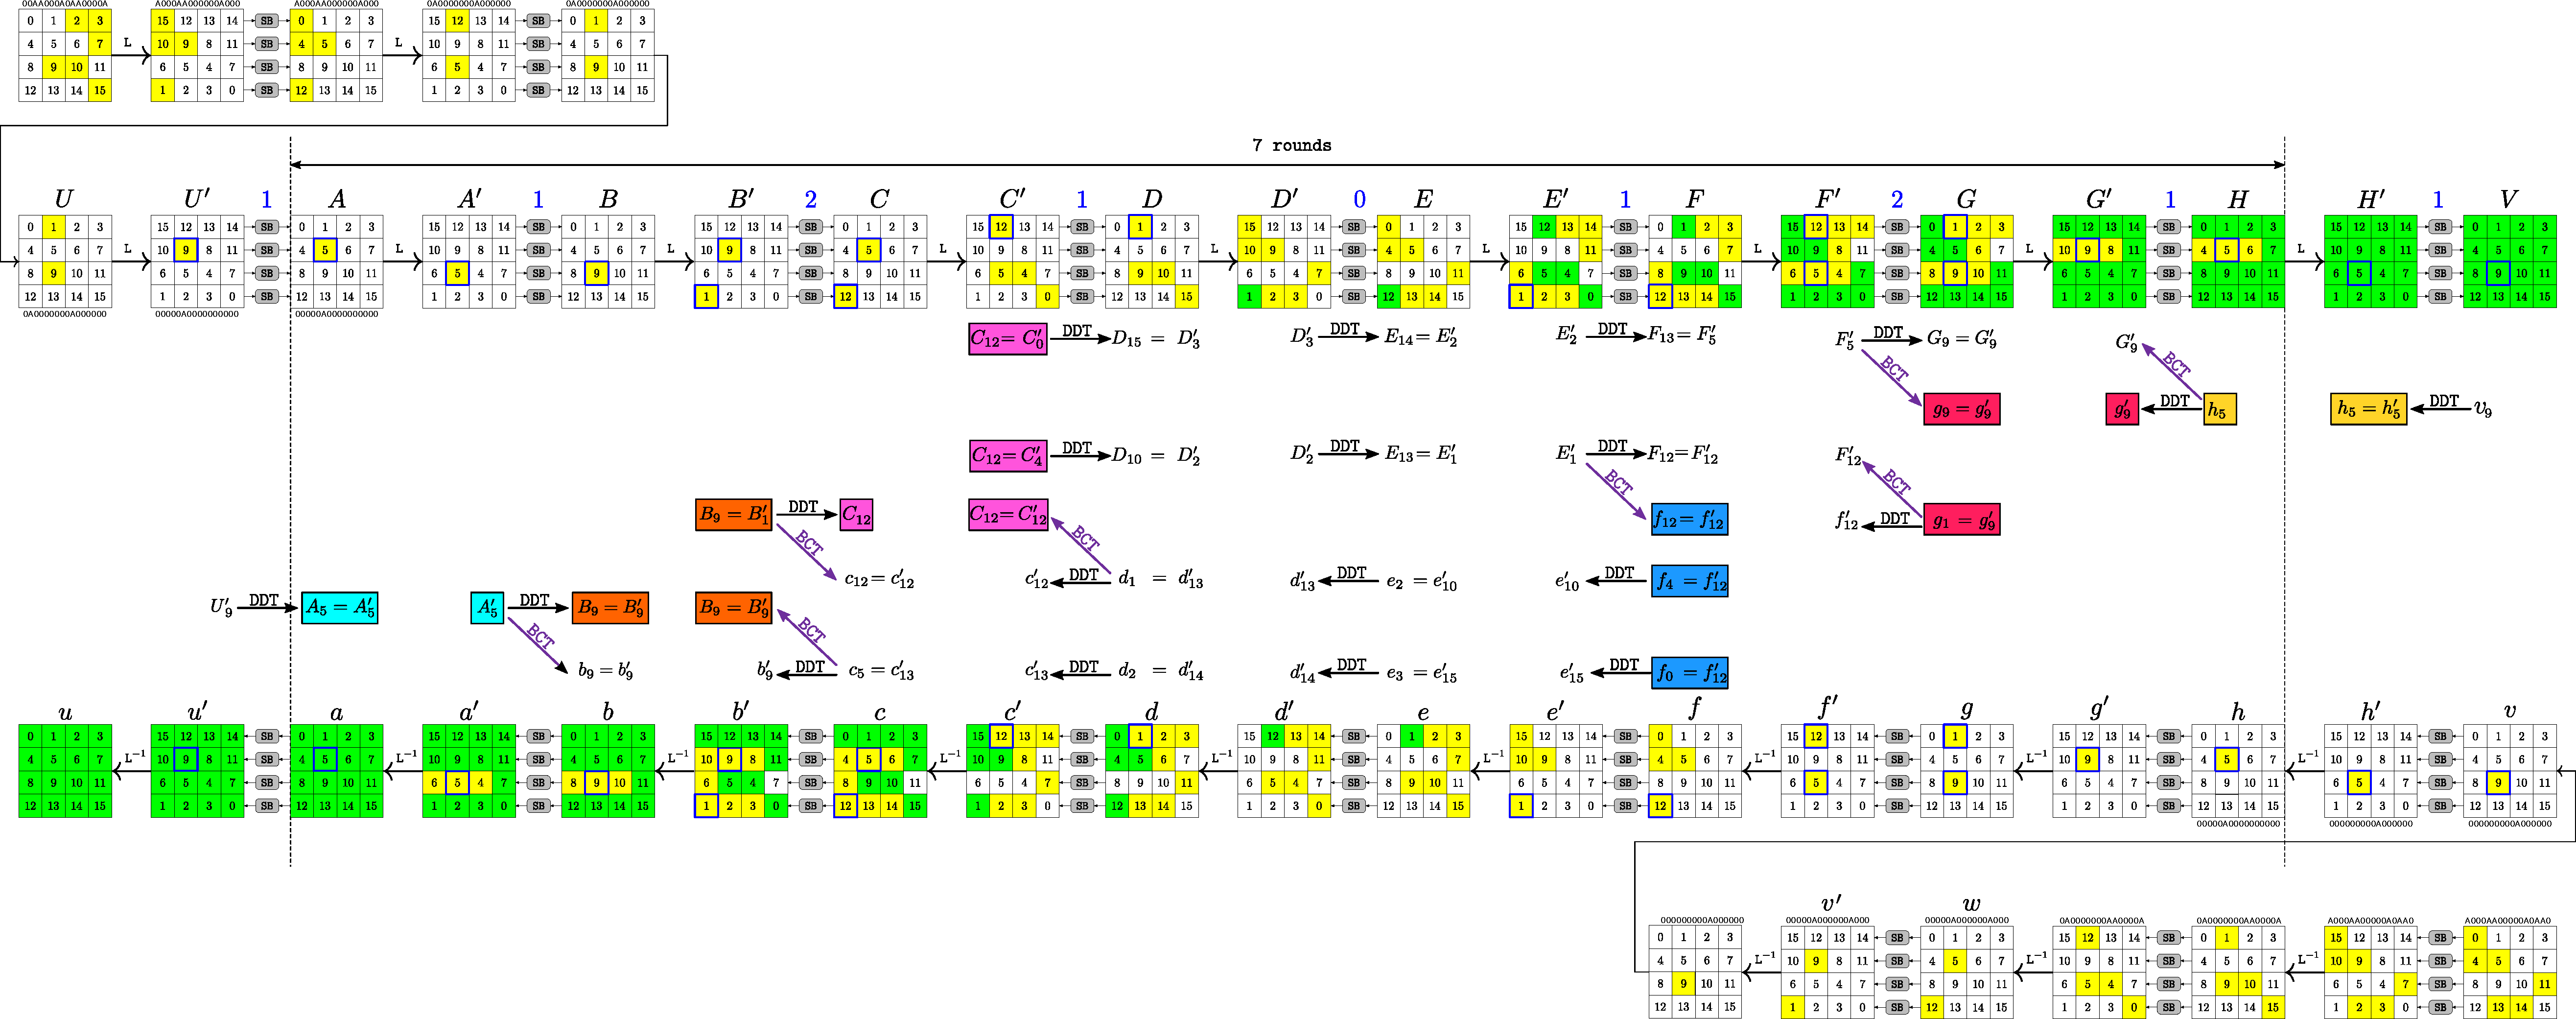
\includegraphics[width=\textwidth]{./figures/middle_part_7r_2.pdf}
\end{figure}
}
\only<2>{
\begin{figure}
\centering
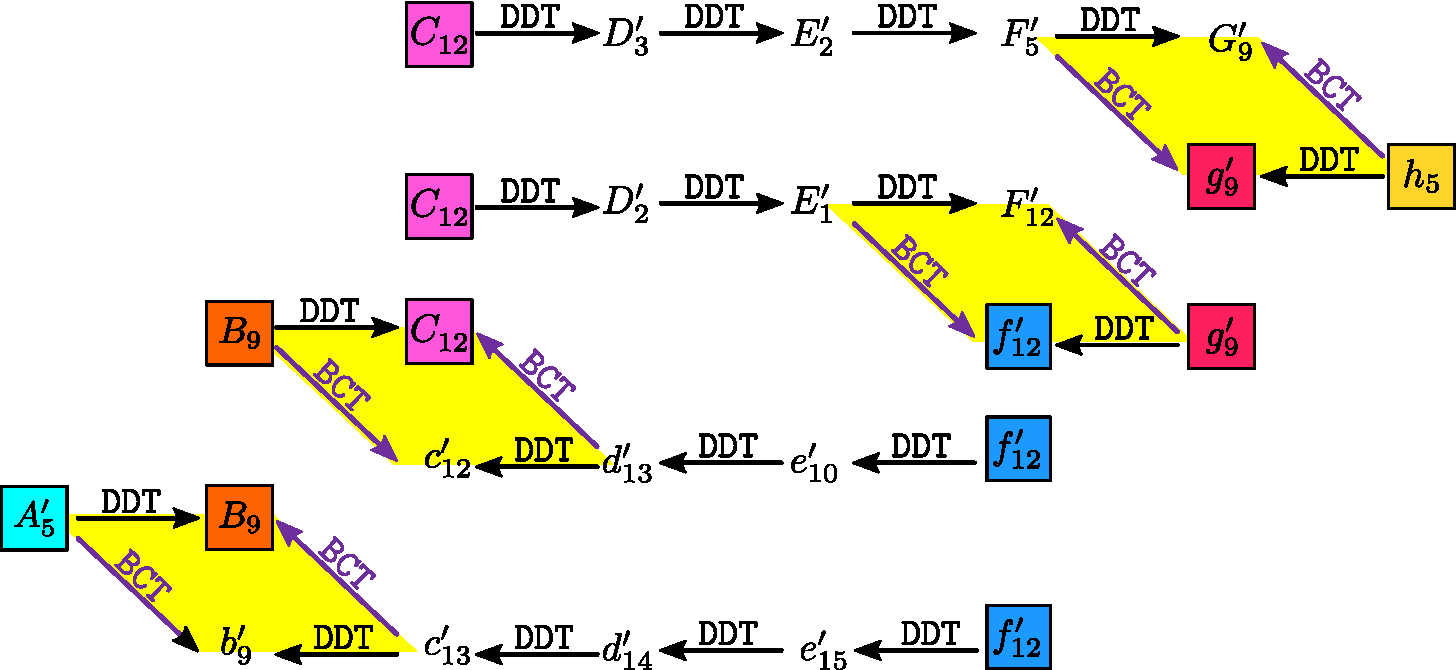
\includegraphics[width=0.6\textwidth]{./figures/middle_part_7r_3.pdf}
\end{figure}
\begin{center}
{\scriptsize $
\texttt{DBCT}_{\text{total}}= \texttt{DBCT}^{\vdash}(A_5, B_{9}, c_5)\cdot \texttt{DBCT}^{\vdash}(B_{9}, C_{12}, d_{1})\cdot\texttt{DBCT}^{\dashv}(E'_1, f'_{12}, g'_{9})
\cdot\texttt{DBCT}^{\dashv}(F'_5, g'_{9}, h_5)$}
{\scriptsize $
\text{Pr}_{\text{total}}= \Pr(d_{1} \xleftarrow{2 ~\ddt} f'_{12})\cdot
\Pr(c_{5} \xleftarrow{3 ~\ddt} f'_{12})\cdot \Pr(C_{12} \xrightarrow{2 ~\ddt} E'_1)\cdot
\Pr(C_{12} \xrightarrow{3 ~\ddt} F'_5)$ }
{\scriptsize
	$r = 2^{-8\cdot n}\cdot\sum_{B_{9}}\sum_{C_{12}}\sum_{g'_{9}}\sum_{f'_{12}}\sum_{c_5}\sum_{d_{1}} \sum_{E'_1}\sum_{F'_5} \dbct_{\text{total}}\cdot \text{Pr}_{\text{total}}$.}
\end{center}
}
\end{frame}

%%%%%%%%%%%%%%%%%%%%%%%%%%%%%%%%%%%%%%%%%%%%%%%%%%%%%%%%%%%%%%%%%%%%%%%%
%%%%%%%%%%%%%%%%%%%%%%%%%%%%%%%%%%%%%%%%%%%%%%%%%%%%%%%%%%%%%%%%%%%%%%%%
\section{Differential-Linear Cryptanalysis}
\sectionheader[\huge\color{tug}\faExchange]{Differential-Linear Cryptanalysis}

%%%%%%%%%%%%%%%%%%%%%%%%%%%%%%%%%%%%%%%%%%%%%%%%%%%%%%%%%%%%%%%%%%%%%%%%
\begin{frame}{Differential-Linear (DL) Attack \cite{dl_crypto_LangfordH94}}
\vspace{-0.2cm}
\begin{columns}
\column[c]{0.7\textwidth}
\begin{itemize}
  \small
  \item $\pr(\Delta\In \xrightarrow{E\Up}\Delta\Mid) = p$
  \item $\corr(\lambda\Mid \xrightarrow{E\Low} \lambda\Out) = q$
  \item Assumptions ($\Delta X = X_{1} \oplus X_{2}$):
  \begin{enumerate}
    \small
    % \item Round independence assumption inside $E\Up, E\Low$
    \item $E\Up$, and $E\Low$ are statistically independent
    \item $\pr\left(\lambda\Mid \cdot \Delta X = 0\right) = 1/2$ when $\Delta X \neq \Delta\Mid$
  \end{enumerate}
  \item $\corr\left(\lambda\Out\cdot C_1 \oplus \lambda\Out\cdot C_2\right) =  (-1)^{\lambda\Mid\cdot\Delta\Mid} \cdot p q^{2} = \pm p q^{2}$
\end{itemize}
\column[c]{0.3\textwidth}
\begin{center}
\begin{tikzpicture}[bc/.style={draw,minimum height=1cm, minimum width=.7cm, rounded corners=2pt}]
  \pgfmathsetmacro{\dx}{3};
  \pgfmathsetmacro{\dy}{2};
  \foreach \i/\labelside in {1/left, 2/right} {
    \draw (\dx*\i,0) node[below]     (P\i)  {$P_\i$}
          ++(0,-\dy) node[bc, fill=upper] (Eu\i) {\textcolor{white}{$E\Up$}}
          ++(0,-\dy) node[bc, fill=lower] (El\i) {\textcolor{white}{$E\Low$}}
          ++(0,-\dy) node[above]    (C\i)  {$C_{\i}$};
    \draw[->] (P\i)  -- coordinate (Pp\i)           (Eu\i);
    \draw[->] (Eu\i) -- coordinate (Xp\i) node[\labelside] {$X_{\i}$} (El\i);
    \draw[->] (El\i) -- coordinate (Cc\i)           (C\i);
  }
  \draw[dashed, <->] (Pp1) -- node[red, above] (Pm) {$\Delta\In$} (Pp2);
  \draw[dashed, <->] (Xp1) -- node[red, above] (Xm) {$\Delta\Mid$} (Xp2);
  \draw[dashed, ->] (Pm)++(0, -\dy/4) -- node[right]{$p$} (Xm);
  \draw (Xp1) ++(0.7,-0.2) node[blue] (Gm1) {$\lambda\Mid$}
        (Xp2) ++(-0.7,-0.2) node[blue] (Gm2) {$\lambda\Mid$};
  \foreach \i/\labelside in {1/left, 2/right} {
    \draw (Gm\i|-C\i) node[blue] (Go\i) {$\lambda_o$};
    \draw[dashed, ->] (Gm\i) -- node[\labelside] {$q$} (Go\i);
    }
  \draw[dashed, ->, gray] (Go1) to[out=90, in=180] ($(Xm)+(0, -0.4)$) to[out=0, in=90] (Go2);
\end{tikzpicture}
\end{center}
\end{columns}
\end{frame}

%%%%%%%%%%%%%%%%%%%%%%%%%%%%%%%%%%%%%%%%%%%%%%%%%%%%%%%%%%%%%%%%%%%%%%%%
\begin{frame}{Differential-Linear Attack Revisited \cite{fse_BlondeauLN14, journals_joc_BlondeauLN17}}
\vspace{-0.2cm}
\begin{columns}
\column[c]{0.7\textwidth}
\begin{itemize}
  \small
  % \item $\pr(\Delta\In \xrightarrow{E\Up}\Delta\Mid) = p$
  \item $\corr(\Lambda X \xrightarrow{E\Low} \lambda\Out) = \corr(\Lambda X, \lambda\Out)$
  \item Assumptions:
  \begin{enumerate}
    % \item Round independence assumption within $E\Up, E\Low$
    \item $E\Up$, and $E\Low$ are statistically independent    
  \end{enumerate}
  \item $\corr(\lambda\Out\cdot C_1 \oplus \lambda\Out\cdot C_2) = \sum_{\Delta X, \Lambda X}
  \corr(\Lambda X \cdot \Delta X) \cdot \corr^{2}(\Lambda X, \lambda\Out)$
\end{itemize}  
\column[c]{0.3\textwidth}
\begin{center}
\begin{tikzpicture}[bc/.style={draw,minimum height=1cm, minimum width=.7cm, rounded corners=2pt}]
  \pgfmathsetmacro{\dx}{3};
  \pgfmathsetmacro{\dy}{2};
  \foreach \i/\labelside in {1/left, 2/right} {
    \draw (\dx*\i,0) node[below]     (P\i)  {$P_\i$}
          ++(0,-\dy) node[bc, fill=upper] (Eu\i) {\textcolor{white}{$E\Up$}}
          ++(0,-\dy) node[bc, fill=lower] (El\i) {\textcolor{white}{$E\Low$}}
          ++(0,-\dy) node[above]    (C\i)  {$C_{\i}$};
    \draw[->] (P\i)  -- coordinate (Pp\i)           (Eu\i);
    \draw[->] (Eu\i) -- coordinate (Xp\i) node[\labelside] {$X_{\i}$} (El\i);
    \draw[->] (El\i) -- coordinate (Cc\i)           (C\i);
  }
  \draw[dashed, <->] (Pp1) -- node[red, above] (Pm) {$\Delta\In$} (Pp2);
  \draw[dashed, <->] (Xp1) -- node[red, above] (Xm) {$\Delta X$} (Xp2);
  \draw[dashed, ->] (Pm)++(0, -\dy/4) -- node[right]{} (Xm);
  \draw (Xp1) ++(0.7,-0.2) node[blue] (Gm1) {$\Lambda X$}
        (Xp2) ++(-0.7,-0.2) node[blue] (Gm2) {$\Lambda X$};
  \foreach \i/\labelside in {1/left, 2/right} {
    \draw (Gm\i|-C\i) node[blue] (Go\i) {$\lambda_o$};
    \draw[dashed, ->] (Gm\i) -- node[\labelside] {} (Go\i);
    }
  \draw[dashed, ->, gray] (Go1) to[out=90, in=180] ($(Xm)+(0, -0.4)$) to[out=0, in=90] (Go2);
\end{tikzpicture}
\end{center}
\end{columns}
\end{frame}

%%%%%%%%%%%%%%%%%%%%%%%%%%%%%%%%%%%%%%%%%%%%%%%%%%%%%%%%%%%%%%%%%%%%%%%%
\begin{frame}{Sandwich Framework for DL Attack \cite{joc_DunkelmanKS14, dlct_eurocrypt_BarOnDKW19}}
\vspace{-0.2cm}
\begin{columns}
\column[c]{0.7\textwidth}
\begin{itemize}
  \small
  \item<1-> $\corrmid(\Delta X, \Lambda Y) = \corr\left(\Lambda Y \cdot E\Mid(X) \oplus \Lambda Y \cdot E\Mid(X \oplus \Delta X)\right)$
  \item<1-> $\corr(\lambda\Out\cdot\Delta C)\!=\!\sum_{\Delta X, \Lambda Y}\pr(\Delta\In, \Delta X) \cdot \corrmid(\Delta X, \Lambda Y) \cdot \corr^{2}(\Lambda Y, \lambda\Out)$
  \item<2-> $\pr(\Delta\In \xrightarrow{E\Up}\Delta\Mid) = p$
  \item<2-> $\corrmid(\Delta\Mid, \lambda\Mid) = r$
  \item<2-> $\corr(\lambda\Mid \xrightarrow{E\Low} \lambda\Out) = q$
  % \item Assumptions:
  % \begin{enumerate}
  %   \item Round independence assumption within $E\Up, E\Low, E\Mid$
  % \end{enumerate}
  \item<2-> $\corr(\lambda\Out\cdot\Delta C) \approx prq^{2}$
\end{itemize}  
\column[c]{0.3\textwidth}
\begin{center}
\begin{tikzpicture}[bc/.style={draw,minimum height=1cm, minimum width=.7cm, rounded corners=2pt}]
  \pgfmathsetmacro{\dx}{3};
  \pgfmathsetmacro{\dy}{1.6};
  \foreach \i/\labelside in {1/left, 2/right} {
    \draw (\dx*\i,0) node[below]     (P\i)  {$P_\i$}
          ++(0,-\dy) node[bc, fill=upper] (Eu\i) {\textcolor{white}{$E\Up$}}
          ++(0,-\dy) node[bc, fill=common] (Em\i) {$E\Mid$}
          ++(0,-\dy) node[bc, fill=lower] (El\i) {\textcolor{white}{$E\Low$}}
          ++(0,-\dy) node[above]    (C\i)  {$C_{\i}$};
    \draw[->] (P\i)  -- coordinate (Pp\i)           (Eu\i);
    \draw[->] (Eu\i) -- coordinate (Xp\i) node[\labelside] {$X_{\i}$} (Em\i);
    \draw[->] (Em\i) -- coordinate (Y\i) node[\labelside] {$Y_{\i}$} (El\i);
    \draw[->] (El\i) -- coordinate (Cc\i)           (C\i);
  }
  \draw[dashed, <->] (Pp1) -- node[red, above] (Pm) {$\Delta\In$} (Pp2);
  \draw[dashed, <->] (Xp1) -- node[red, above] (Xm) {\only<1>{$\Delta X$}\only<2>{$\Delta \Mid$}} (Xp2);
  \draw[dashed, ->] (Pm)++(0, -\dy/4) -- node[right]{$p$} (Xm);
  \draw (Y1)++(0.5,0) node[blue] (Gm1) {\only<1>{$\Lambda Y$}\only<2>{$\lambda\Mid$}}
        (Y2)++(-0.5,0) node[blue] (Gm2) {\only<1>{$\Lambda Y$}\only<2>{$\lambda\Mid$}};
  \draw[dashed, ->] (Gm1) to[out=90, in=180] ($(Xm)+(0, -0.4)$) node[below] {$r$} to[out=0, in=90] (Gm2);
  \foreach \i/\labelside in {1/right, 2/left} {
    \draw (Gm\i|-C\i) node[blue] (Go\i) {$\lambda_o$};
    \draw[dashed, ->] (Gm\i) -- node[\labelside] {$q$} (Go\i);
    }
\end{tikzpicture}
\end{center}
\end{columns}
\end{frame}

%%%%%%%%%%%%%%%%%%%%%%%%%%%%%%%%%%%%%%%%%%%%%%%%%%%%%%%%%%%%%%%%%%%%%%%%
\begin{frame}{Differential-Linear Connectivity Table (\dlct)}
\vspace{-0.4cm}
\begin{columns}
\column[c]{0.8\textwidth}
\begin{center}
  \begin{block}{Differential-Linear Connectivity Table (\dlct) \cite{dlct_eurocrypt_BarOnDKW19}}
  \small
  For a vectorial Boolean function $S: \mathbb{F}_{2}^{n} \rightarrow \mathbb{F}_{2}^{m}$, the \dlct of $S$ is a $2^{n}\times 2^{m}$ table whose rows correspond to the input difference $\Delta\In$ to $S$ and whose columns correspond to the output mask $\lambda\Out$ of $S$.
  The entry at index $(\Delta\In, \lambda\Out)$ is
  \[\dlct(\Delta\In, \lambda\Out) = |\dlct_0(\Delta\In, \lambda\Out)| - |\dlct_1(\Delta\In, \lambda\Out)|,\]
  where $\dlct_b(\Delta\In, \lambda\Out) = \{x\in \mathbb{F}_{2}^{n}:~ \lambda\Out \cdot S(x) \oplus \lambda\Out \cdot S(x \oplus \Delta\In) = b\}$.
  \end{block}
  $\corr_{\dlct}\left(\Delta\In, \lambda\Out\right) = 2^{-n}\cdot\dlct\left(\Delta\In, \lambda\Out\right)$
\end{center}
\column[c]{0.2\textwidth}
\begin{center}
\tikzset{bc/.style={draw,minimum height=.5cm, minimum width=.5cm, rounded corners=2pt, fill=white}}
\begin{tikzpicture}
  \pgfmathsetmacro{\dx}{2};
  \pgfmathsetmacro{\dy}{2};
  \foreach \i/\labelside/\maskside in {1/left/right, 2/right/left} {
    \draw (\dx*\i,0)    node[below]                (P\i)  {$X_\i$}
          ++(0,-\dy)    node[bc]                   (Eu\i) {$\mathcal{S}$}
          ++(0,-\dy)    node[above]                (C\i)  {$Y_{\i}$}
            (C\i)       node[\maskside=.3cm,blue] (L\i)  {$\lambda\Out$};
    \draw[->] (P\i)  -- coordinate (Pp\i)  (Eu\i);
    \draw[->] (Eu\i) -- coordinate (Cc\i)  (C\i);
  }
  \draw[dashed, <->, gray] (Pp1) -- node[red, above] (Pm) {$\Delta\In$} (Pp2);
  \draw[dashed, ->, gray] (L1) -- (L1|-Eu1.south) to[out=90,in=90,looseness=2] (L2|-Eu2.south) -- (L2);
\end{tikzpicture}
\smallskip\\
\begin{tikzpicture}
  \pgfmathsetmacro{\lth}{1.5};
  \pgfmathsetmacro{\htt}{0.5};
  \node[red] (D1) at (0, 0) {$\Delta\In$};
  \node[right=\lth of D1, gray] (D2) {$\Delta\Out$};
  \node[below=\htt of D1, gray] (L1) {$\lambda\In$};
  \node[right=\lth of L1, blue] (L2) {$\lambda\Out$};
  \draw[->, gray] (D1) -- (D2);
  \draw[->] (D1) -- (L2);
  \draw[<-, gray] (L1) -- (L2);
\end{tikzpicture}
\end{center}
\end{columns}
\end{frame}

%%%%%%%%%%%%%%%%%%%%%%%%%%%%%%%%%%%%%%%%%%%%%%%%%%%%%%%%%%%%%%%%%%%%%%%%
%%%%%%%%%%%%%%%%%%%%%%%%%%%%%%%%%%%%%%%%%%%%%%%%%%%%%%%%%%%%%%%%%%%%%%%%
\section{Generalized DLCT Framework}
\sectionheader[\huge\color{tug}\faLightbulbO]{Generalized DLCT Framework}

%%%%%%%%%%%%%%%%%%%%%%%%%%%%%%%%%%%%%%%%%%%%%%%%%%%%%%%%%%%%%%%%%%%%%%%%
\begin{frame}{Upper Differential-Linear Connectivity Table (\udlct)}
\vspace{-0.4cm}
\begin{columns}
\column[c]{0.8\textwidth}
\begin{center}
  \begin{block}{Upper Differential-Linear Connectivity Table (\udlct)}
  \small
  For a vectorial Boolean function $S: \mathbb{F}_{2}^{n} \rightarrow \mathbb{F}_{2}^{m}$, the \udlct of $S$ is a $2^{n}\times 2^{n} \times 2^{m}$ table.
  The entry at index $(\Delta\In, \Delta\Out, \lambda\Out)$ is
  \[\udlct(\Delta\In, \Delta\Out, \lambda\Out) = |\udlct_0(\Delta\In, \Delta\Out, \lambda\Out)| - |\udlct_1(\Delta\In, \Delta\Out, \lambda\Out)|,\]
  where $\udlct_b(\Delta\In, \Delta\Out, \lambda\Out) = \{x\in \mathbb{F}_{2}^{n}:~S(x) \oplus  S(x \oplus \Delta\In) = \Delta\Out  \text{~and~} \lambda\Out \cdot \Delta\Out = b\}$.
  \end{block}
  $\corr_{\udlct}\left(\Delta\In, \Delta\Out, \lambda\Out\right) = 2^{-n}\cdot\udlct\left(\Delta\In, \Delta\Out, \lambda\Out\right)$
\end{center}
\column[c]{0.2\textwidth}
\begin{center}
\tikzset{bc/.style={draw,minimum height=.5cm, minimum width=.5cm, rounded corners=2pt, fill=white}}
\begin{tikzpicture}
  \pgfmathsetmacro{\dx}{2};
  \pgfmathsetmacro{\dy}{2};
  \foreach \i/\labelside/\maskside in {1/left/right, 2/right/left} {
    \draw (\dx*\i,0)    node[below]                (P\i)  {$X_\i$}
          ++(0,-\dy)    node[bc]                   (Eu\i) {$\mathcal{S}$}
          ++(0,-\dy)    node[above]                (C\i)  {$Y_{\i}$}
            (C\i)       node[\maskside=.3cm,blue] (L\i)  {$\lambda\Out$};
    \draw[->] (P\i)  -- coordinate (Pp\i)  (Eu\i);
    \draw[->] (Eu\i) -- coordinate (Cc\i)  (C\i);
  }
  \draw[dashed, <->, gray] (Pp1) -- node[red, above] (Pm) {$\Delta\In$} (Pp2);
  \draw[dashed, ->, gray] (L1) -- (L1|-Eu1.south) to[out=90,in=90,looseness=2] (L2|-Eu2.south) -- (L2);
\end{tikzpicture}
\smallskip\\
\begin{tikzpicture}
  \pgfmathsetmacro{\lth}{1.5};
  \pgfmathsetmacro{\htt}{0.5};
  \node[red] (D1) at (0, 0) {$\Delta\In$};
  \node[right=\lth of D1, red] (D2) {$\Delta\Out$};
  \node[below=\htt of D1, gray] (L1) {$\lambda\In$};
  \node[right=\lth of L1, blue] (L2) {$\lambda\Out$};
  \draw[->] (D1) -- (D2);
  \draw[->] (D1) -- (L2);
  \draw[<-, gray] (L1) -- (L2);
\end{tikzpicture}
\end{center}
\end{columns}
\end{frame}

%%%%%%%%%%%%%%%%%%%%%%%%%%%%%%%%%%%%%%%%%%%%%%%%%%%%%%%%%%%%%%%%%%%%%%%%
\begin{frame}{Lower Differential-Linear Connectivity Table (\ldlct)}
\vspace{-0.4cm}
\begin{columns}
\column[c]{0.8\textwidth}
\begin{center}
  \begin{block}{Lower Differential-Linear Connectivity Table (\ldlct)}
    \small
    For a vectorial Boolean function $S: \mathbb{F}_{2}^{n} \rightarrow \mathbb{F}_{2}^{m}$, the \ldlct of $S$ is a $2^{n} \times 2^{m} \times 2^{m}$ table.
    The entry at index $(\Delta\In, \lambda\In, \lambda_o)$ is
  \[\ldlct(\Delta\In, \lambda\In, \lambda\Out) = |\ldlct_0(\Delta\In, \lambda\In, \lambda\Out)| - |\ldlct_1(\Delta\In, \lambda\In, \lambda\Out)|,\]
where $\ldlct_b(\Delta\In, \lambda\In, \lambda\Out) = \{x\in \mathbb{F}_{2}^{n}:~ \lambda\In \cdot \Delta\In \oplus \lambda\Out \cdot S(x) \oplus \lambda\Out \cdot S(x \oplus \Delta\In) = b \}$.
  \end{block}
  $\corr_{\ldlct}\left(\Delta\In, \lambda\In, \lambda\Out\right) = 2^{-n}\cdot\ldlct\left(\Delta\In, \lambda\In, \lambda\Out\right)$
\end{center}
\column[c]{0.2\textwidth}
\begin{center}
\tikzset{bc/.style={draw,minimum height=.5cm, minimum width=.5cm, rounded corners=2pt, fill=white}}
\begin{tikzpicture}
  \pgfmathsetmacro{\dx}{2};
  \pgfmathsetmacro{\dy}{2};
  \foreach \i/\labelside/\maskside in {1/left/right, 2/right/left} {
    \draw (\dx*\i,0)    node[below]                (P\i)  {$X_\i$}
          ++(0,-\dy)    node[bc]                   (Eu\i) {$\mathcal{S}$}
          ++(0,-\dy)    node[above]                (C\i)  {$Y_{\i}$}
            (C\i)       node[\maskside=.3cm,blue] (L\i)  {$\lambda\Out$};
    \draw[->] (P\i)  -- coordinate (Pp\i)  (Eu\i);
    \draw[->] (Eu\i) -- coordinate (Cc\i)  (C\i);
  }
  \draw[dashed, <->, gray] (Pp1) -- node[red, above] (Pm) {$\Delta\In$} (Pp2);
  \draw[dashed, ->, gray] (L1) -- (L1|-Eu1.south) to[out=90,in=90,looseness=2] (L2|-Eu2.south) -- (L2);
\end{tikzpicture}
\smallskip\\
\begin{tikzpicture}
  \pgfmathsetmacro{\lth}{1.5};
  \pgfmathsetmacro{\htt}{0.5};
  \node[red] (D1) at (0, 0) {$\Delta\In$};
  \node[right=\lth of D1, gray] (D2) {$\Delta\Out$};
  \node[below=\htt of D1, blue] (L1) {$\lambda\In$};
  \node[right=\lth of L1, blue] (L2) {$\lambda\Out$};
  \draw[->, gray] (D1) -- (D2);
  \draw[->] (D1) -- (L2);
  \draw[<-] (L1) -- (L2);
\end{tikzpicture}
\end{center}
\end{columns}
\end{frame}

%%%%%%%%%%%%%%%%%%%%%%%%%%%%%%%%%%%%%%%%%%%%%%%%%%%%%%%%%%%%%%%%%%%%%%%%
\begin{frame}{Extended Differential-Linear Connectivity Table (\edlct)}
\vspace{-0.4cm}
\begin{columns}
\column[c]{0.8\textwidth}
\begin{center}
  \begin{block}{Extended Differential-Linear Connectivity Table (\edlct)}
    \small
    For a vectorial Boolean function $S: \mathbb{F}_{2}^{n} \rightarrow \mathbb{F}_{2}^{m}$, the \edlct of $S$ is a $2^{n} \times 2^{n} \times 2^{m} \times 2^{m}$ table.
    The entry at index $(\Delta_i, \Delta_o, \lambda_i, \lambda_o)$ is
    \[\edlct(\Delta\In, \Delta\Out, \lambda\In, \lambda\Out)\!=\!|\edlct_0(\Delta\In,\!\Delta\Out,\!\lambda\In,\!\lambda\Out)| - |\edlct_1(\Delta\In,\!\Delta\Out,\!\lambda\In,\!\lambda\Out)|,\]
    where $\edlct_b(\Delta\In, \Delta\Out, \lambda\In, \lambda\Out) = \{x\in \mathbb{F}_{2}^{n}:~ S(x) \oplus  S(x \oplus \Delta\In) = \Delta\Out \text{~and~} \lambda\In \cdot \Delta\In \oplus \lambda\Out \cdot \Delta\Out = b\}$.
  \end{block}
  $\corr_{\edlct}\left(\Delta\In, \Delta\Out, \lambda\In, \lambda\Out\right) = 2^{-n}\cdot\edlct\left(\Delta\In, \Delta\Out, \lambda\In, \lambda\Out\right)$
\end{center}
\column[c]{0.2\textwidth}
\begin{center}
\tikzset{bc/.style={draw,minimum height=.5cm, minimum width=.5cm, rounded corners=2pt, fill=white}}
\begin{tikzpicture}
  \pgfmathsetmacro{\dx}{2};
  \pgfmathsetmacro{\dy}{2};
  \foreach \i/\labelside/\maskside in {1/left/right, 2/right/left} {
    \draw (\dx*\i,0)    node[below]                (P\i)  {$X_\i$}
          ++(0,-\dy)    node[bc]                   (Eu\i) {$\mathcal{S}$}
          ++(0,-\dy)    node[above]                (C\i)  {$Y_{\i}$}
            (C\i)       node[\maskside=.3cm,blue] (L\i)  {$\lambda\Out$};
    \draw[->] (P\i)  -- coordinate (Pp\i)  (Eu\i);
    \draw[->] (Eu\i) -- coordinate (Cc\i)  (C\i);
  }
  \draw[dashed, <->, gray] (Pp1) -- node[red, above] (Pm) {$\Delta\In$} (Pp2);
  \draw[dashed, ->, gray] (L1) -- (L1|-Eu1.south) to[out=90,in=90,looseness=2] (L2|-Eu2.south) -- (L2);
\end{tikzpicture}
\smallskip\\
\begin{tikzpicture}
  \pgfmathsetmacro{\lth}{1.5};
  \pgfmathsetmacro{\htt}{0.5};
  \node[red] (D1) at (0, 0) {$\Delta\In$};
  \node[right=\lth of D1, red] (D2) {$\Delta\Out$};
  \node[below=\htt of D1, blue] (L1) {$\lambda\In$};
  \node[right=\lth of L1, blue] (L2) {$\lambda\Out$};
  \draw[->] (D1) -- (D2);
  \draw[->] (D1) -- (L2);
  \draw[<-] (L1) -- (L2);
\end{tikzpicture}
\end{center}
\end{columns}
\end{frame}

%%%%%%%%%%%%%%%%%%%%%%%%%%%%%%%%%%%%%%%%%%%%%%%%%%%%%%%%%%%%%%%%%%%%%%%%
\begin{frame}{Double Differential-Linear Connectivity Table (\ddlct)}
\begin{columns}
\column[c]{0.75\textwidth}
\begin{center}
\begin{tikzpicture}
  \pgfmathsetmacro{\lth}{1.5};
  \pgfmathsetmacro{\htt}{0.5};
  \node[red] (D1) at (0, 0) {$\Delta\In$};
  \node[right=\lth of D1, gray] (D2) {$\Delta\Mid$};
  \node[right=\lth of D2, gray] (D3) {$\Delta\Out$};
  \node[below=\htt of D1, gray] (L1) {$\lambda\In$};
  \node[right=\lth of L1, gray] (L2) {$\lambda\Mid$};
  \node[right=\lth of L2, blue] (L3) {$\lambda\Out$};
  \draw[->] (D1) -- (D2);
  \draw[->, gray] (D2) -- (D3);
  \draw[->] (D1) -- (L2);
  \draw[->, gray] (L1) -- (L2);
  \draw[->, lower] (L2) -- (L3);
  \draw[->] (D2) -- (L3);
\end{tikzpicture}
\begin{equation*}
\footnotesize
\ddlct(\Delta\In, \lambda\Out) = 2^{-n}\!\cdot\!\sum_{\Delta\Mid}\sum_{\lambda\Mid}  \udlct\left(\Delta\In, \Delta\Mid, \lambda\Mid\right) \cdot \ldlct\left(\Delta\Mid, \lambda\Mid, \lambda\Out\right)
\end{equation*}
\end{center}
\column[c]{0.25\textwidth}
\begin{tikzpicture}
  \pgfdeclarelayer{foreground}
  \pgfdeclarelayer{background}
  \pgfsetlayers{background,main,foreground}
  \tikzset{bc/.style={draw,minimum height=.5cm, minimum width=.5cm, rounded corners=2pt, fill=white}}
  \pgfmathsetmacro{\dx}{2};
  \pgfmathsetmacro{\dy}{1.5};
  \foreach \i/\labelside/\maskside in {1/left/right, 2/right/left} {
    \draw (\dx*\i,0)    node[below]                (P\i)  {$X_\i$}
          ++(0,-\dy)    node[bc]                   (Eu\i) {$\mathcal{S}$}
          ++(0,-.6*\dy) coordinate[xor]            (x\i)
                        node[\labelside=.4cm]      (K\i)  {$\$$}
          ++(0,-.3*\dy) node[minimum size=.3cm]    (dd\i) {}
          ++(0,-.6*\dy) node[bc]                   (El\i) {$\mathcal{S}$}
          ++(0,-\dy)    node[above]                (C\i)  {$Y_{\i}$}
            (C\i)       node[\maskside=.3cm,blue] (L\i)  {$\lambda\Out$};
    \draw[->] (P\i)  -- coordinate (Pp\i)  (Eu\i);
    \draw[->] (Eu\i) --                    (x\i);
    \draw[->] (K\i)  --                    (x\i);
    \draw[  ] (x\i)  --                    (dd\i);
    \draw[->] (dd\i) --                    (El\i);
    \draw[->] (El\i) -- coordinate (Cc\i)  (C\i);
    \draw[dotted,thick] (dd\i.north)  --   (dd\i.south);
  }
  \draw[dashed, <->, gray] (Pp1) -- node[red, above] (Pm) {$\Delta\In$} (Pp2);
  \draw[dashed, ->, gray] (L1) -- (L1|-Eu1.south) to[out=90,in=90,looseness=2] (L2|-Eu2.south) -- (L2);
\end{tikzpicture}
\end{columns}
\end{frame}

%%%%%%%%%%%%%%%%%%%%%%%%%%%%%%%%%%%%%%%%%%%%%%%%%%%%%%%%%%%%%%%%%%%%%%%%
\begin{frame}{Generalized \dlct Framework (GBCT)}
\vspace{-0.3cm}
\begin{itemize}
\item How to formulate the correaltion for more than 1 round?
\begin{figure}
  \centering
  \begin{subfigure}{0.3\textwidth}
      \centering
      \begin{tikzpicture}
        \pgfmathsetmacro{\lth}{1.5};
        \pgfmathsetmacro{\htt}{0.5};
        \node[red] (D1) at (0, 0) {$\Delta\In$};
        \node[right=\lth of D1, gray] (D2) {$\Delta\Out$};
        \node[below=\htt of D1, gray] (L1) {$\lambda\In$};
        \node[right=\lth of L1, blue] (L2) {$\lambda\Out$};
        \draw[->, gray] (D1) -- (D2);
        \draw[->] (D1) -- (L2);
        \draw[->, gray] (L1) -- (L2);
      \end{tikzpicture}
      \caption*{$\dlct\left(\Delta\In, \lambda\Out\right)$}
  \end{subfigure}
  \begin{subfigure}{0.3\textwidth}
      \centering
      \begin{tikzpicture}
        \pgfmathsetmacro{\lth}{1.5};
        \pgfmathsetmacro{\htt}{0.5};
        \node[red] (D1) at (0, 0) {$\Delta\In$};
        \node[right=\lth of D1, red] (D2) {$\Delta\Out$};
        \node[below=\htt of D1, gray] (L1) {$\lambda\In$};
        \node[right=\lth of L1, blue] (L2) {$\lambda\Out$};
        \draw[->] (D1) -- (D2);
        \draw[->] (D1) -- (L2);
        \draw[->, gray] (L1) -- (L2);
      \end{tikzpicture}
      \caption*{$\udlct\left(\Delta\In, \Delta\Out, \lambda\Out\right)$}
  \end{subfigure}
  \begin{subfigure}{0.3\textwidth}
      \centering
      \begin{tikzpicture}
        \pgfmathsetmacro{\lth}{1.5};
        \pgfmathsetmacro{\htt}{0.5};
        \node[red] (D1) at (0, 0) {$\Delta\In$};
        \node[right=\lth of D1, gray] (D2) {$\Delta\Out$};
        \node[below=\htt of D1, blue] (L1) {$\lambda\In$};
        \node[right=\lth of L1, blue] (L2) {$\lambda\Out$};
        \draw[->, gray] (D1) -- (D2);
        \draw[->] (D1) -- (L2);
        \draw[->] (L1) -- (L2);
      \end{tikzpicture}
      \caption*{$\ldlct\left(\Delta\In, \lambda\In, \lambda\Out\right)$}
  \end{subfigure}
  \bigskip

  \begin{subfigure}{0.4\textwidth}
      \centering
      \begin{tikzpicture}
        \pgfmathsetmacro{\lth}{1.5};
        \pgfmathsetmacro{\htt}{0.5};
        \node[red] (D1) at (0, 0) {$\Delta\In$};
        \node[right=\lth of D1, red] (D2) {$\Delta\Out$};
        \node[below=\htt of D1, blue] (L1) {$\lambda\In$};
        \node[right=\lth of L1, blue] (L2) {$\lambda\Out$};
        \draw[->] (D1) -- (D2);
        \draw[->] (D1) -- (L2);
        \draw[->] (L1) -- (L2);
      \end{tikzpicture}
      \caption*{$\edlct\left(\Delta\In, \Delta\Out, \lambda\In, \lambda\Out\right)$}
  \end{subfigure}
  \begin{subfigure}{0.5\textwidth}
      \centering
      \begin{tikzpicture}
        \pgfmathsetmacro{\lth}{1.5};
        \pgfmathsetmacro{\htt}{0.5};
        \node[red] (D1) at (0, 0) {$\Delta\In$};
        \node[right=\lth of D1, gray] (D2) {$\Delta\Mid$};
        \node[right=\lth of D2, gray] (D3) {$\Delta\Out$};
        \node[below=\htt of D1, gray] (L1) {$\lambda\In$};
        \node[right=\lth of L1, gray] (L2) {$\lambda\Mid$};
        \node[right=\lth of L2, blue] (L3) {$\lambda\Out$};
        \draw[->] (D1) -- (D2);
        \draw[->, gray] (D2) -- (D3);
        \draw[->] (D1) -- (L2);
        \draw[->, gray] (L1) -- (L2);
        \draw[->, lower] (L2) -- (L3);
        \draw[->] (D2) -- (L3);
      \end{tikzpicture}
      \caption*{$\ddlct\left(\Delta\In, \lambda\Out\right)$}
  \end{subfigure}
\end{figure}
\end{itemize}
\end{frame}

%%%%%%%%%%%%%%%%%%%%%%%%%%%%%%%%%%%%%%%%%%%%%%%%%%%%%%%%%%%%%%%%%%%%%%%%
\begin{frame}{Application of the Generalized \dlct Tables - AES ({\scriptsize\protect\dlfeistellegend})}
\vspace{-0.3cm}
\begin{figure}
%\resizebox{\textwidth}{!}{%
%\centering
%\input{aes_example.tex}
%}
  \colorlet{myred}{upper}
  \colorlet{myblue}{lower}
  \colorlet{mygray}{tuggray!50}
  \centering
  \begin{tikzpicture}[>=latex, 
                      stateopts/.style={scale=.35},
                      fillopts/.style={blue!50},
                      cellopts/.style={font=\scriptsize\color{white}}]
    \pgfmathsetmacro{\stepsep}{2} % between two cells with a labeled edge

    \draw[every node/.style={state}, rounded corners=2pt]
          (0,0)        node (S0) {\State{\Fill[myred]{ss32}\Cell{ss32}{\texttt{01}}}}
        ++(\stepsep,0) node (S1) {\State{\Fill[myred]{ss32}\Cell{ss32}{$\alpha$}}}
        ++(\stepsep,0) node (S2) {\State{\FillColumn[myred]{3}\Cell{ss03}{$\alpha$}\Cell{ss13}{$\alpha$}\Cell{ss23}{$3\alpha$}\Cell{ss33}{$2\alpha$}}}
        ++(\stepsep,0) node (S3) {\State{\FillColumn[mygray]{3}\Fill[myred]{ss03}\Cell{ss03}{$\beta$}}}
        ++(\stepsep,0) node (S4) {\State{\FillState[mygray]\FillColumn[myred]{3}\Cell{ss03}{$2\beta$}\Cell{ss13}{$3\beta$}\Cell{ss23}{$\beta$}\Cell{ss33}{$\beta$}}}
        ++(\stepsep,0) node (S5) {\State{\FillState[mygray]}}
        ;

    \foreach \in/\out/\label in {S0/S1/SB,S1/S2/{SR\\MC\\AK},
                                  S2/S3/SB,S3/S4/{SR\\MC\\AK},
                                  S4/S5/SB} {
    \draw[->] (\in) --node[above,align=center,font=\sffamily\tiny]{\label} (\out);
  }
  \foreach \st/\rr in {0/0, 2/1, 4/2} {
    \draw (S\st.north west) node[above right,font=\small] {R\rr};
  }
  \end{tikzpicture}
  \bigskip

  \begin{tikzpicture}[>=latex, 
                      stateopts/.style={scale=.35},
                      fillopts/.style={blue!50},
                      cellopts/.style={font=\scriptsize\color{white}}]
    \pgfmathsetmacro{\stepsep}{2} % between two cells with a labeled edge

    \draw[every node/.style={state}, rounded corners=2pt]
          (0,0)        node (S0) {\State{\FillState[mygray]}}
        ++(\stepsep,0) node (S1) {\State{\FillState[mygray]\FillDiagonal[myblue]{3}\Cell{ss03}{$2\delta$}\Cell{ss10}{$3\delta$}\Cell{ss21}{$\delta$}\Cell{ss32}{$\delta$}}}
        ++(\stepsep,0) node (S2) {\State{\FillDiagonal[mygray]{3}\Fill[myblue]{ss03}\Cell{ss03}{$\delta$}}}
        ++(\stepsep,0) node (S3) {\State{\FillDiagonal[myblue]{3}\Cell{ss03}{$\gamma$}\Cell{ss10}{$\gamma$}\Cell{ss21}{$2\gamma$}\Cell{ss32}{$3\gamma$}}}
        ++(\stepsep,0) node (S4) {\State{\Fill[myblue]{ss23}\Cell{ss23}{$\gamma$}}}
        ++(\stepsep,0) node (S5) {\State{\Fill[myblue]{ss23}\Cell{ss23}{\texttt{09}}}}
        ;

    \foreach \in/\out/\label in {S0/S1/SB,S1/S2/{SR\\MC\\AK},
                                  S2/S3/SB,S3/S4/{SR\\MC\\AK},
                                  S4/S5/SB} {
    \draw[->] (\in) --node[above,align=center,font=\sffamily\tiny]{\label} (\out);
  }
  \foreach \st/\rr in {0/0, 2/1, 4/2} {
    \draw (S\st.south west) node[below right,font=\small] {R\rr};
  }
  \end{tikzpicture}
\end{figure}
\[\sum_{\alpha, \beta, \gamma, \delta} \mathbb{C}_{\udlct}({\tt 1},\alpha,\delta) \cdot \mathbb{C}_{\edlct}(\alpha,\beta,\delta,\gamma)\cdot \mathbb{C}_{\ldlct}(\beta,\gamma,{\tt 9}) = -2^{-7.94}\]
\end{frame}

%%%%%%%%%%%%%%%%%%%%%%%%%%%%%%%%%%%%%%%%%%%%%%%%%%%%%%%%%%%%%%%%%%%%%%%%
\begin{frame}{Application of the Generalized \dlct Tables - TWINE ({\scriptsize\protect\dlfeistellegend})}
\vspace{-0.8cm}
\begin{columns}
\column[c]{0.40\textwidth}
\begin{figure}
  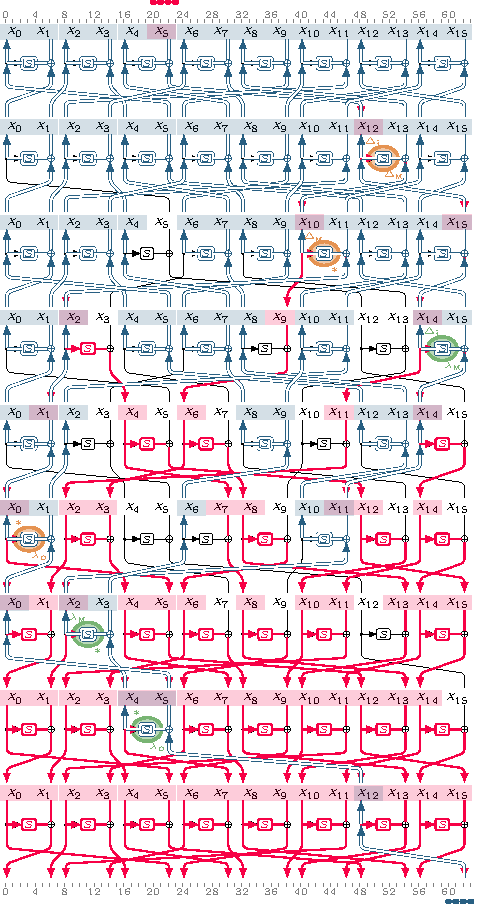
\includegraphics[width=0.60\textwidth, clip]{./figures/twine_double_dlct_example_1.pdf}
\end{figure}
\column[c]{0.60\textwidth}
{
\scriptsize
\begin{align*}
  \corr(\Delta\In, \lambda\Out) =& \sum_{\Delta\Mid} \pr_{\ddt}(\Delta\In, \Delta\Mid) \cdot \corr_{\ddlct}\left(\Delta\Mid, \lambda\Out\right)\\
                                            =& \sum_{\lambda\Mid} \corr_{\ddlct}\left(\Delta\In, \lambda\Mid\right) \cdot \corr^{2}_{\lat}\left(\lambda\Mid, \lambda\Out\right).\\
  \corr_{tot}(\Delta\In, \lambda\Out)       =& \corr^{2}(\Delta\In, \lambda\Out).
\end{align*}}
\smallskip
\resizebox{!}{0.16\textwidth}{
\begin{tabular}{ccc}
  \toprule
  Input/Output Differences/Linear-mask & Formula & Exp. Correlation\\
  \midrule
  $(\Delta\In, \lambda\Out) = (\texttt{0xb4}, \texttt{0x67})$ & $-2^{-7.66}$ & $-2^{-7.64}$ \\
  $(\Delta\In, \lambda\Out) = (\texttt{0x02}, \texttt{0x02})$ & $-2^{-7.92}$ & $-2^{-7.93}$ \\
  $(\Delta\In, \lambda\Out) = (\texttt{0x55}, \texttt{0x55})$ & $-2^{-7.99}$ & $-2^{-7.98}$ \\
  $(\Delta\In, \lambda\Out) = (\texttt{0xbf}, \texttt{0xef})$ & $-2^{-8.05}$ & $-2^{-8.06}$ \\
  $(\Delta\In, \lambda\Out) = (\texttt{0xfe}, \texttt{0x06})$ & $-2^{-8.26}$ & $-2^{-8.25}$ \\
  $(\Delta\In, \lambda\Out) = (\texttt{0x4b}, \texttt{0x1a})$ & $-2^{-8.43}$ & $-2^{-8.44}$ \\
  \bottomrule
\end{tabular}
}
\end{columns}
\end{frame}

%%%%%%%%%%%%%%%%%%%%%%%%%%%%%%%%%%%%%%%%%%%%%%%%%%%%%%%%%%%%%%%%%%%%%%%%
%%%%%%%%%%%%%%%%%%%%%%%%%%%%%%%%%%%%%%%%%%%%%%%%%%%%%%%%%%%%%%%%%%%%%%%%
\section{Differential-Linear Switches and Deterministic Trails}
\sectionheader[\huge\color{tug}\faLightbulbO\faLightbulbO]{Differential-Linear Switches and Deterministic Trails}

%%%%%%%%%%%%%%%%%%%%%%%%%%%%%%%%%%%%%%%%%%%%%%%%%%%%%%%%%%%%%%%%%%%%%%%%
\begin{frame}{Cell-Wise and Bit-Wise Switches}
  \sparen
  \sparen
  \begin{center}
  \scalebox{0.55}{
  \begin{tabular}{@{}l*{16}{r}@{}}
      \toprule
      $x$                & 0 & 1 & 2 & 3 & 4 & 5 & 6 & 7 & 8 & 9 & a & b & c & d & e & f \\
      \midrule
      $\mathcal{S}  (x)$ & 4 & 0 & a & 7 & b & e & 1 & d & 9 & f & 6 & 8 & 5 & 2 & c & 3 \\
      \bottomrule
    \end{tabular}
  }
  \sparen
  \sparen
  \end{center}
  \begin{columns}
  % \column[c]{0.10\textwidth}
  % \begin{center}
  %   \scalebox{0.65}{%
  %   \begin{tikzpicture}
  %     \draw (0,0) node[box, name=S, minimum size=2cm] {$\mathcal{S}$};
  %     \foreach \i/\a in {1/123,2/101,3/78,4/56} {
  %       \draw (S.\a) node[above=2ex] (x\i) {$x_{\i}$};
  %       \draw (x\i|-S.south) node[below=2ex] (y\i) {$y_{\i}$};
  %       \draw[next] (x\i) -- (x\i|-S.north);
  %       \draw[next] (y\i|-S.south) -- (y\i);
  %     }

  %     \draw (y2) node[tug] {$y_2$};
  %     \draw (x1) node[tug] {$x_1$};
  %     \draw (x4) node[tug] {$x_4$};

  %     \draw[] (x1.south-|S.west) rectangle (x4.north-|S.east);
  %     \draw[] (y1.south-|S.west) rectangle (y4.north-|S.east);

  %     \foreach \i/\dir in {x1/above, x4/above, y2/below} {\draw (\i) node[\dir=2.5ex, tug] (m\i) {1};}
  %     \foreach \i/\dir in {x2/above, x3/above, y1/below, y3/below, y4/below} {\draw (\i) node[\dir=2.5ex] (m\i) {0};}

  %     \draw[thick] (mx1.south-|S.west) rectangle (mx4.north-|S.east);
  %     \draw[thick] (my1.south-|S.west) rectangle (my4.north-|S.east);

  %     \draw (mx4) node[right=3ex] (alpha) {$\Delta\In$};
  %     \draw (x4-|alpha) node              {$x$};
  %     \draw (y4-|alpha) node              {$\mathcal{S}(x)$};
  %     \draw (my4-|alpha) node             {$\lambda\Out$};
      
  %   \end{tikzpicture}
  %   }
  % \end{center}
  \column[c]{0.55\textwidth}
  \begin{center}
    \scalebox{0.55}{      
      \newcommand{\es}{}
      \begin{tabular}{@{}r|*{3}c*{13}{c}@{}}
        \toprule
        $\Delta$\,\textbackslash\,$\lambda$ & \es\texttt{0}\es & \es\texttt{1}\es & \es\texttt{2}\es & \es\texttt{3}\es & \es\texttt{4}\es & \es\texttt{5}\es & \es\texttt{6}\es & \es\texttt{7}\es & \es\texttt{8}\es & \es\texttt{9}\es & \es\texttt{a}\es & \es\texttt{b}\es & \es\texttt{c}\es & \es\texttt{d}\es & \es\texttt{e}\es & \es\texttt{f}\es \\
        \midrule
        \texttt{0\,} & 16 & 16 & 16 & 16 & 16 & 16 & 16 & 16 & 16 & 16 & 16 & 16 & 16 & 16 & 16 & 16\\
        \texttt{1\,} & 16 & 0 & 0 & 0 & \cellcolor{upper}\textcolor{white}{-16} & 0 & 0 & 0 & 0 & 0 & 0 & 0 & 0 & 0 & 0 & 0\\
        \texttt{2\,} & 16 & -8 & -8 & 0 & 0 & 0 & 8 & -8 & 0 & -8 & 0 & 8 & 0 & 0 & 0 & 0\\
        \texttt{3\,} & 16 & 0 & -8 & -8 & 0 & -8 & 8 & 0 & 0 & 0 & 0 & 0 & 0 & -8 & 0 & 8\\
        \texttt{4\,} & 16 & 0 & -8 & 0 & 0 & 0 & -8 & 0 & \cellcolor{upper}\textcolor{white}{-16} & 0 & 8 & 0 & 0 & 0 & 8 & 0\\
        \texttt{5\,} & 16 & 0 & -8 & 0 & 0 & 0 & -8 & 0 & 0 & 0 & 8 & 0 & \cellcolor{upper}\textcolor{white}{-16} & 0 & 8 & 0\\
        \texttt{6\,} & 16 & -8 & 8 & -8 & 0 & 0 & -8 & 0 & 0 & -8 & 0 & 0 & 0 & 0 & 0 & 8\\
        \texttt{7\,} & 16 & 0 & 8 & 0 & 0 & -8 & -8 & -8 & 0 & 0 & 0 & 8 & 0 & -8 & 0 & 0\\
        \texttt{8\,} & 16 & 0 & 0 & 0 & \cellcolor{upper}\textcolor{white}{-16} & 0 & 0 & 0 & \cellcolor{upper}\textcolor{white}{-16} & 0 & 0 & 0 & \cellcolor{upper}\textcolor{white}{16} & 0 & 0 & 0\\
        \texttt{9\,} & 16 & -8 & 0 & -8 & \cellcolor{upper}\textcolor{white}{16} & -8 & 0 & -8 & 0 & 8 & 0 & -8 & 0 & 8 & 0 & -8\\
        \texttt{a\,} & 16 & 0 & 0 & 8 & 0 & 8 & 0 & 0 & 0 & 0 & -8 & 0 & 0 & -8 & -8 & -8\\
        \texttt{b\,} & 16 & 8 & 0 & 0 & 0 & 0 & 0 & 8 & 0 & -8 & -8 & -8 & 0 & 0 & -8 & 0\\
        \texttt{c\,} & 16 & 0 & 0 & -8 & 0 & 0 & 0 & -8 & \cellcolor{upper}\textcolor{white}{16} & 0 & 0 & -8 & 0 & 0 & 0 & -8\\
        \texttt{d\,} & 16 & -8 & 0 & 0 & 0 & -8 & 0 & 0 & 0 & 8 & 0 & 0 & \cellcolor{upper}\textcolor{white}{-16} & 8 & 0 & 0\\
        \texttt{e\,} & 16 & 0 & 0 & 0 & 0 & 8 & 0 & 8 & 0 & 0 & -8 & -8 & 0 & -8 & -8 & 0\\
        \texttt{f\,} & 16 & 8 & 0 & 8 & 0 & 0 & 0 & 0 & 0 & -8 & -8 & 0 & 0 & 0 & -8 & -8\\
        \bottomrule
      \end{tabular}
    }
  \end{center}
  \column[c]{0.45\textwidth}
  \begin{itemize}
    \footnotesize
    \item<2-> Cell-wise switches: $\dlct(\Delta\In, 0) = \dlct(0, \lambda\Out) = 2^{n}$ for all $\Delta\In, \lambda\Out$
    \item<3-> Bit-wise switches: $\dlct(\Delta\In, \lambda\Out) = \pm 2^{n}$ for $\Delta\In, \lambda\Out \neq 0$
    \begin{itemize}
      \footnotesize
      \item<3-> Example: $\corr\left(\texttt{9}, \texttt{4}\right) = \frac{16}{16}$
    \end{itemize}
  \end{itemize}
\end{columns}
\end{frame}

%%%%%%%%%%%%%%%%%%%%%%%%%%%%%%%%%%%%%%%%%%%%%%%%%%%%%%%%%%%%%%%%%%%%%%%%
\begin{frame}{\small Deterministic Bit-Wise Differential Trails (Forward)}
  \sparen
  \sparen
  \begin{center}
  \scalebox{0.55}{
  \begin{tabular}{@{}l*{16}{r}@{}}
      \toprule
      $x$                & 0 & 1 & 2 & 3 & 4 & 5 & 6 & 7 & 8 & 9 & a & b & c & d & e & f \\
      \midrule
      $\mathcal{S}  (x)$ & 4 & 0 & a & 7 & b & e & 1 & d & 9 & f & 6 & 8 & 5 & 2 & c & 3 \\
      \bottomrule
    \end{tabular}
  }
  \sparen
  \sparen
  \end{center}
  \begin{columns}
  % \column[c]{0.10\textwidth}
  % \begin{center}
  %   \scalebox{0.65}{%
  %   \begin{tikzpicture}
  %     \draw (0,0) node[box, name=S, minimum size=2cm] {$\mathcal{S}$};
  %     \foreach \i/\a in {1/123,2/101,3/78,4/56} {
  %       \draw (S.\a) node[above=2ex] (x\i) {$x_{\i}$};
  %       \draw (x\i|-S.south) node[below=2ex] (y\i) {$y_{\i}$};
  %       \draw[next] (x\i) -- (x\i|-S.north);
  %       \draw[next] (y\i|-S.south) -- (y\i);
  %     }

  %     % \draw (y3) node[tug] {$y_3$};
  %     % \draw (x1) node[tug] {$x_1$};
  %     % \draw (x4) node[tug] {$x_4$};

  %     \draw[] (x1.south-|S.west) rectangle (x4.north-|S.east);
  %     \draw[] (y1.south-|S.west) rectangle (y4.north-|S.east);
      
  %     \visible<1>{
  %     \foreach \i/\dir in {x1/above, x2/above, x3/above, x4/above, y1/below, y2/below, y3/below, y4/below} {\draw (\i) node[\dir=2.5ex, tug] (m\i) {\bf 0};}
  %     \foreach \i/\dir in {} {\draw (\i) node[\dir=2.5ex] (m\i) {\bf 1};}
  %     \foreach \i/\dir in {} {\draw (\i) node[tugblue, \dir=2.5ex] (m\i) {\bf ?};}
  %     }
  %     \visible<2>{
  %     \foreach \i/\dir in {x1/above, x2/above, x3/above} {\draw (\i) node[\dir=2.5ex, tug] (m\i) {\bf 0};}
  %     \foreach \i/\dir in {x4/above, y2/below} {\draw (\i) node[\dir=2.5ex] (m\i) {\bf 1};}
  %     \foreach \i/\dir in {y1/below, y3/below, y4/below} {\draw (\i) node[tugblue, \dir=2.5ex] (m\i) {\bf ?};}
  %     }
  %     \visible<3>{
  %     \foreach \i/\dir in {x1/above, x3/above, x4/above} {\draw (\i) node[\dir=2.5ex, tug] (m\i) {\bf 0};}
  %     \foreach \i/\dir in {x2/above, y1/below} {\draw (\i) node[\dir=2.5ex] (m\i) {\bf 1};}
  %     \foreach \i/\dir in {y2/below, y3/below, y4/below} {\draw (\i) node[tugblue, \dir=2.5ex] (m\i) {\bf ?};}
  %     }
  %     \visible<4>{
  %     \foreach \i/\dir in {x2/above, x3/above, x4/above} {\draw (\i) node[\dir=2.5ex, tug] (m\i) {\bf 0};}
  %     \foreach \i/\dir in {x1/above, y1/below, y2/below} {\draw (\i) node[\dir=2.5ex] (m\i) {\bf 1};}
  %     \foreach \i/\dir in {y3/below, y4/below} {\draw (\i) node[tugblue, \dir=2.5ex] (m\i) {\bf ?};}
  %     }
  %     \visible<5>{
  %     \foreach \i/\dir in {x2/above, x3/above, y2/below} {\draw (\i) node[\dir=2.5ex, tug] (m\i) {\bf 0};}
  %     \foreach \i/\dir in {x1/above, x4/above} {\draw (\i) node[\dir=2.5ex] (m\i) {\bf 1};}
  %     \foreach \i/\dir in {y1/below, y3/below, y4/below} {\draw (\i) node[tugblue, \dir=2.5ex] (m\i) {\bf ?};}
  %     }
  %     \visible<6>{
  %     \foreach \i/\dir in {x3/above, x4/above, y1/below} {\draw (\i) node[\dir=2.5ex, tug] (m\i) {\bf 0};}  
  %     \foreach \i/\dir in {x1/above, x2/above} {\draw (\i) node[\dir=2.5ex] (m\i) {\bf 1};}
  %     \foreach \i/\dir in {y2/below, y3/below, y4/below} {\draw (\i) node[tugblue, \dir=2.5ex] (m\i) {\bf ?};}
  %     }
      
  %     \draw[thick] (mx1.south-|S.west) rectangle (mx4.north-|S.east);
  %     \draw[thick] (my1.south-|S.west) rectangle (my4.north-|S.east);

  %     \draw (mx1) node[left=3ex] (alpha) {$\Delta_{i}$};
  %     \draw (x1-|alpha) node            {$x$};
  %     \draw (y1-|alpha) node            {$\mathcal{S}(x)$};
  %     \draw (my1-|alpha) node            {$\Delta_{o}$};
      
  %   \end{tikzpicture}
  %   }
  % \end{center}
  \column[c]{0.60\textwidth}
  \begin{center}
    \scalebox{0.55}{      
      \newcommand{\es}{}
      \begin{tabular}{@{}c|*{3}c*{13}{c}@{}}
        \toprule
        $\Delta_{i}$\,\textbackslash\,$\Delta_{o}$ & \es\texttt{0}\es & \es\texttt{1}\es & \es\texttt{2}\es & \es\texttt{3}\es & \es\texttt{4}\es & \es\texttt{5}\es & \es\texttt{6}\es & \es\texttt{7}\es & \es\texttt{8}\es & \es\texttt{9}\es & \es\texttt{a}\es & \es\texttt{b}\es & \es\texttt{c}\es & \es\texttt{d}\es & \es\texttt{e}\es & \es\texttt{f}\es \\
        \midrule
        \rowcolor<1->{red!50}
        \texttt{0\,} & 16 & 0 & 0 & 0 & 0 & 0 & 0 & 0 & 0 & 0 & 0 & 0 & 0 & 0 & 0 & 0\\
        \rowcolor<1->{red!50}
        \texttt{1\,} & 0 & 0 & 0 & 0 & 2 & 2 & 2 & 2 & 0 & 0 & 0 & 0 & 2 & 2 & 2 & 2\\
        \texttt{2\,} & 0 & 2 & 0 & 2 & 0 & 0 & 0 & 4 & 0 & 2 & 2 & 0 & 0 & 0 & 2 & 2\\
        \texttt{3\,} & 0 & 2 & 0 & 2 & 0 & 0 & 4 & 0 & 0 & 2 & 2 & 0 & 0 & 0 & 2 & 2\\
        \rowcolor<1->{red!50}
        \texttt{4\,} & 0 & 0 & 0 & 0 & 0 & 0 & 0 & 0 & 0 & 0 & 4 & 4 & 2 & 2 & 2 & 2\\
        \texttt{5\,} & 0 & 0 & 0 & 0 & 2 & 2 & 2 & 2 & 0 & 0 & 4 & 4 & 0 & 0 & 0 & 0\\
        \texttt{6\,} & 0 & 2 & 0 & 2 & 0 & 4 & 0 & 0 & 0 & 2 & 2 & 0 & 2 & 2 & 0 & 0\\
        \texttt{7\,} & 0 & 2 & 0 & 2 & 4 & 0 & 0 & 0 & 0 & 2 & 2 & 0 & 2 & 2 & 0 & 0\\
        \rowcolor<1->{red!50}
        \texttt{8\,} & 0 & 0 & 0 & 0 & 0 & 0 & 0 & 0 & 0 & 0 & 0 & 0 & 4 & 4 & 4 & 4\\
        \rowcolor<1->{red!50}
        \texttt{9\,} & 0 & 4 & 4 & 0 & 0 & 0 & 0 & 0 & 0 & 4 & 0 & 4 & 0 & 0 & 0 & 0\\
        \texttt{a\,} & 0 & 0 & 2 & 2 & 2 & 0 & 0 & 2 & 4 & 0 & 0 & 0 & 0 & 2 & 0 & 2\\
        \texttt{b\,} & 0 & 0 & 2 & 2 & 0 & 2 & 2 & 0 & 4 & 0 & 0 & 0 & 2 & 0 & 2 & 0\\
        \rowcolor<1->{red!50}
        \texttt{c\,} & 0 & 4 & 4 & 0 & 2 & 2 & 2 & 2 & 0 & 0 & 0 & 0 & 0 & 0 & 0 & 0\\
        \texttt{d\,} & 0 & 0 & 0 & 0 & 2 & 2 & 2 & 2 & 0 & 4 & 0 & 4 & 0 & 0 & 0 & 0\\
        \texttt{e\,} & 0 & 0 & 2 & 2 & 0 & 2 & 2 & 0 & 4 & 0 & 0 & 0 & 0 & 2 & 0 & 2\\
        \texttt{f\,} & 0 & 0 & 2 & 2 & 2 & 0 & 0 & 2 & 4 & 0 & 0 & 0 & 2 & 0 & 2 & 0\\
        \bottomrule
      \end{tabular}
    }
  \end{center}
  \column[c]{0.40\textwidth}  
  \begin{equation*}
    {\footnotesize
    \begin{alignedat}{3}
      &\textcolor{tugred}{\Delta_{i} = (0, 0, 0, 0) \xrightarrow{S} \Delta_{o} = (0, 0, 0, 0)}\\
      % &\textcolor{tugblue}{\Delta_{i} \neq (0, 0, 0, 0) \xrightarrow{S} \Delta_{o} \neq (0, 0, 0, 0)}\\
      &\textcolor{tugred}{\Delta_{i} = (0, 0, 0, 1) \xrightarrow{S} \Delta_{o} = (?, 1, ?, ?)}\\
      &\textcolor{tugred}{\Delta_{i} = (0, 1, 0, 0) \xrightarrow{S} \Delta_{o} = (1, ?, ?, ?)}\\
      &\textcolor{tugred}{\Delta_{i} = (1, 0, 0, 0) \xrightarrow{S} \Delta_{o} = (1, 1, ?, ?)}\\
      &\textcolor{tugred}{\Delta_{i} = (1, 0, 0, 1) \xrightarrow{S} \Delta_{o} = (?, 0, ?, ?)}\\
      &\textcolor{tugred}{\Delta_{i} = (1, 1, 0, 0) \xrightarrow{S} \Delta_{o} = (0, ?, ?, ?)}
      \end{alignedat}
    }
  \end{equation*}
\end{columns}
\end{frame}

%%%%%%%%%%%%%%%%%%%%%%%%%%%%%%%%%%%%%%%%%%%%%%%%%%%%%%%%%%%%%%%%%%%%%%%
\begin{frame}{\small Deterministic Bit-Wise Linear Trails (Backward)}
  \sparen
  \sparen
  \begin{center}
  \scalebox{0.55}{
  \begin{tabular}{@{}l*{16}{r}@{}}
      \toprule
      $x$                & 0 & 1 & 2 & 3 & 4 & 5 & 6 & 7 & 8 & 9 & a & b & c & d & e & f \\
      \midrule
      $\mathcal{S}  (x)$ & 4 & 0 & a & 7 & b & e & 1 & d & 9 & f & 6 & 8 & 5 & 2 & c & 3 \\
      \bottomrule
    \end{tabular}
  }
  \sparen
  \sparen
  \end{center}
  \begin{columns}
  % \column[c]{0.10\textwidth}
  % \begin{center}
  %   \scalebox{0.65}{%
  %   \begin{tikzpicture}
  %     \draw (0,0) node[box, name=S, minimum size=2cm] {$\mathcal{S}$};
  %     \foreach \i/\a in {1/123,2/101,3/78,4/56} {
  %       \draw (S.\a) node[above=2ex] (x\i) {$x_{\i}$};
  %       \draw (x\i|-S.south) node[below=2ex] (y\i) {$y_{\i}$};
  %       \draw[next] (x\i) -- (x\i|-S.north);
  %       \draw[next] (y\i|-S.south) -- (y\i);
  %     }

  %     % \draw (y3) node[tug] {$y_3$};
  %     % \draw (x1) node[tug] {$x_1$};
  %     % \draw (x4) node[tug] {$x_4$};

  %     \draw[] (x1.south-|S.west) rectangle (x4.north-|S.east);
  %     \draw[] (y1.south-|S.west) rectangle (y4.north-|S.east);
      
  %     \visible<1>{
  %     \foreach \i/\dir in {x1/above, x2/above, x3/above, x4/above, y1/below, y2/below, y3/below, y4/below} {\draw (\i) node[\dir=2.5ex, tug] (m\i) {\bf 0};}
  %     \foreach \i/\dir in {} {\draw (\i) node[\dir=2.5ex] (m\i) {\bf 1};}
  %     \foreach \i/\dir in {} {\draw (\i) node[tugblue, \dir=2.5ex] (m\i) {\bf ?};}
  %     }
  %     \visible<2>{
  %     \foreach \i/\dir in {x1/above, x2/above, x4/above} {\draw (\i) node[\dir=2.5ex, tug] (m\i) {\bf 0};}
  %     \foreach \i/\dir in {x3/above, y1/below} {\draw (\i) node[\dir=2.5ex] (m\i) {\bf 1};}
  %     \foreach \i/\dir in {y2/below, y3/below, y4/below} {\draw (\i) node[tugblue, \dir=2.5ex] (m\i) {\bf ?};}
  %     }
  %     \visible<3>{
  %     \foreach \i/\dir in {x2/above, x3/above, x4/above} {\draw (\i) node[\dir=2.5ex, tug] (m\i) {\bf 0};}
  %     \foreach \i/\dir in {x1/above, y1/below, y3/below} {\draw (\i) node[\dir=2.5ex] (m\i) {\bf 1};}
  %     \foreach \i/\dir in {y2/below, y4/below} {\draw (\i) node[tugblue, \dir=2.5ex] (m\i) {\bf ?};}
  %     }
  %     \visible<4>{
  %     \foreach \i/\dir in {x2/above, x4/above, y1/below} {\draw (\i) node[\dir=2.5ex, tug] (m\i) {\bf 0};}
  %     \foreach \i/\dir in {x1/above, x3/above, y4/below} {\draw (\i) node[\dir=2.5ex] (m\i) {\bf 1};}
  %     \foreach \i/\dir in {y2/below, y3/below} {\draw (\i) node[tugblue, \dir=2.5ex] (m\i) {\bf ?};}
  %     }
      
  %     \draw[thick] (mx1.south-|S.west) rectangle (mx4.north-|S.east);
  %     \draw[thick] (my1.south-|S.west) rectangle (my4.north-|S.east);

  %     \draw (mx1) node[left=3ex] (alpha) {$\lambda_{i}$};
  %     \draw (x1-|alpha) node            {$x$};
  %     \draw (y1-|alpha) node            {$\mathcal{S}(x)$};
  %     \draw (my1-|alpha) node            {$\lambda_{o}$};
      
  %   \end{tikzpicture}
  %   }
  % \end{center}
  \column[c]{0.60\textwidth}
  \begin{center}
    \scalebox{0.55}{      
      \newcommand{\es}{}
      \begin{tabular}{@{}c|*{3}{c}c>{\columncolor{blue!20}}c*{3}{c}>{\columncolor{blue!20}}c*{3}{c}>{\columncolor{blue!20}}c*{3}{c}@{}}
        \toprule
        $\lambda_{i}$\,\textbackslash\,$\lambda_{o}$ & \es\texttt{0}\es & \es\texttt{1}\es & \es\texttt{2}\es & \es\texttt{3}\es & \es\texttt{4}\es & \es\texttt{5}\es & \es\texttt{6}\es & \es\texttt{7}\es & \es\texttt{8}\es & \es\texttt{9}\es & \es\texttt{a}\es & \es\texttt{b}\es & \es\texttt{c}\es & \es\texttt{d}\es & \es\texttt{e}\es & \es\texttt{f}\es \\
        \midrule        
        \texttt{0\,} & 16 & 0 & 0 & 0 & 0 & 0 & 0 & 0 & 0 & 0 & 0 & 0 & 0 & 0 & 0 & 0\\
        \texttt{1\,} & 0 & 0 & 4 & -4 & 0 & -8 & -4 & -4 & 0 & 0 & 4 & -4 & -8 & 0 & 4 & 4\\
        \texttt{2\,} & 0 & 0 & 0 & 0 & 0 & 0 & 0 & 0 & 0 & 8 & 8 & 0 & 0 & 8 & -8 & 0\\
        \texttt{3\,} & 0 & -8 & 4 & 4 & 0 & 0 & -4 & 4 & 0 & 0 & -4 & 4 & -8 & 0 & -4 & -4\\
        \texttt{4\,} & 0 & 4 & 0 & 4 & 0 & 4 & 8 & -4 & 0 & 4 & 0 & 4 & -8 & -4 & 0 & 4\\
        \texttt{5\,} & 0 & 4 & -4 & -8 & 0 & -4 & -4 & 0 & 0 & 4 & -4 & 8 & 0 & -4 & -4 & 0\\
        \texttt{6\,} & 0 & -4 & 8 & 4 & 0 & -4 & 0 & -4 & 0 & 4 & 0 & 4 & 8 & -4 & 0 & 4\\
        \texttt{7\,} & 0 & 4 & 4 & 0 & 0 & -4 & 4 & -8 & 0 & -4 & -4 & 0 & 0 & 4 & -4 & -8\\
        \texttt{8\,} & 0 & 0 & 0 & 0 & 0 & 0 & 0 & 0 & 0 & 0 & 8 & 8 & 0 & 0 & 8 & -8\\
        \texttt{9\,} & 0 & 0 & -4 & 4 & 8 & 0 & -4 & -4 & 0 & 0 & 4 & -4 & 0 & -8 & -4 & -4\\
        \texttt{a\,} & 0 & 8 & 0 & 8 & 0 & -8 & 0 & 8 & 0 & 0 & 0 & 0 & 0 & 0 & 0 & 0\\
        \texttt{b\,} & 0 & 0 & -4 & 4 & -8 & 0 & -4 & -4 & 0 & 8 & -4 & -4 & 0 & 0 & 4 & -4\\
        \texttt{c\,} & 0 & 4 & 0 & 4 & 0 & 4 & -8 & -4 & 8 & -4 & 0 & 4 & 0 & 4 & 0 & 4\\
        \texttt{d\,} & 0 & 4 & 4 & 0 & -8 & 4 & -4 & 0 & -8 & -4 & 4 & 0 & 0 & -4 & -4 & 0\\
        \texttt{e\,} & 0 & 4 & 8 & -4 & 0 & 4 & 0 & 4 & 8 & 4 & 0 & -4 & 0 & -4 & 0 & -4\\
        \texttt{f\,} & 0 & -4 & -4 & 0 & -8 & -4 & 4 & 0 & 8 & -4 & 4 & 0 & 0 & -4 & -4 & 0\\
        \bottomrule
      \end{tabular}
    }
  \end{center}
  \column[c]{0.40\textwidth}  
  \begin{equation*}
    {\footnotesize
    \begin{alignedat}{3}
      &\textcolor{blue}{\lambda\In = (1, ?, ?, 1) \xleftarrow{S} \lambda\Out = (0, 1, 0, 0)}\\
      % &\textcolor{tugblue}{\lambda_{i} \neq (0, 0, 0, 0) \xrightarrow{S} \lambda_{o} \neq (0, 0, 0, 0)}\\
      &\textcolor{blue}{\lambda\In = (1, 1, ?, ?) \xleftarrow{S} \lambda\Out = (1, 0, 0, 0)}\\
      &\textcolor{blue}{\lambda\In = (0, ?, ?, ?) \xleftarrow{S} \lambda\Out = (1, 1, 0, 0)}\\
      \end{alignedat}
    }
  \end{equation*}
\end{columns}
\end{frame}

%%%%%%%%%%%%%%%%%%%%%%%%%%%%%%%%%%%%%%%%%%%%%%%%%%%%%%%%%%%%%%%%%%%%%%%%
\begin{frame}{Bit-Wise Switches and Deterministic Trails}
\sparen
\sparen
\begin{center}
\scalebox{0.55}{
\begin{tabular}{@{}l*{16}{r}@{}}
    \toprule
    $x$                & 0 & 1 & 2 & 3 & 4 & 5 & 6 & 7 & 8 & 9 & a & b & c & d & e & f \\
    \midrule
    $\mathcal{S}  (x)$ & 4 & 0 & a & 7 & b & e & 1 & d & 9 & f & 6 & 8 & 5 & 2 & c & 3 \\
    \bottomrule
  \end{tabular}
}
\sparen
\sparen
\end{center}
\begin{columns}
\column[c]{0.55\textwidth}
\begin{center}
  \scalebox{0.55}{      
    \newcommand{\es}{}
      \begin{tabular}{@{}c|*{3}{c}c>{\columncolor{blue!20}}c*{3}{c}>{\columncolor{blue!20}}c*{3}{c}>{\columncolor{blue!20}}c*{3}{c}@{}}
      \toprule
      $\Delta$\,\textbackslash\,$\lambda$ & \es\texttt{0}\es & \es\texttt{1}\es & \es\texttt{2}\es & \es\texttt{3}\es & \es\texttt{4}\es & \es\texttt{5}\es & \es\texttt{6}\es & \es\texttt{7}\es & \es\texttt{8}\es & \es\texttt{9}\es & \es\texttt{a}\es & \es\texttt{b}\es & \es\texttt{c}\es & \es\texttt{d}\es & \es\texttt{e}\es & \es\texttt{f}\es \\
      \midrule      
      \texttt{0\,} & 16 & 16 & 16 & 16 & 16 & 16 & 16 & 16 & 16 & 16 & 16 & 16 & 16 & 16 & 16 & 16\\
      \rowcolor<1->{red!20}
      \texttt{1\,} & 16 & 0 & 0 & 0 & \cellcolor{upper}\textcolor{white}{-16} & 0 & 0 & 0 & 0 & 0 & 0 & 0 & 0 & 0 & 0 & 0\\
      \texttt{2\,} & 16 & -8 & -8 & 0 & 0 & 0 & 8 & -8 & 0 & -8 & 0 & 8 & 0 & 0 & 0 & 0\\
      \texttt{3\,} & 16 & 0 & -8 & -8 & 0 & -8 & 8 & 0 & 0 & 0 & 0 & 0 & 0 & -8 & 0 & 8\\
      \rowcolor<1->{red!20}
      \texttt{4\,} & 16 & 0 & -8 & 0 & 0 & 0 & -8 & 0 & \cellcolor{upper}\textcolor{white}{-16} & 0 & 8 & 0 & 0 & 0 & 8 & 0\\
      \texttt{5\,} & 16 & 0 & -8 & 0 & 0 & 0 & -8 & 0 & 0 & 0 & 8 & 0 & \cellcolor{cyan}-16 & 0 & 8 & 0\\
      \texttt{6\,} & 16 & -8 & 8 & -8 & 0 & 0 & -8 & 0 & 0 & -8 & 0 & 0 & 0 & 0 & 0 & 8\\
      \texttt{7\,} & 16 & 0 & 8 & 0 & 0 & -8 & -8 & -8 & 0 & 0 & 0 & 8 & 0 & -8 & 0 & 0\\
      \rowcolor<1->{red!20}
      \texttt{8\,} & 16 & 0 & 0 & 0 & \cellcolor{upper}\textcolor{white}{-16} & 0 & 0 & 0 & \cellcolor{upper}\textcolor{white}{-16} & 0 & 0 & 0 & \cellcolor{upper}\textcolor{white}{16} & 0 & 0 & 0\\
      \rowcolor<1->{red!20}
      \texttt{9\,} & 16 & -8 & 0 & -8 & \cellcolor{upper}\textcolor{white}{16} & -8 & 0 & -8 & 0 & 8 & 0 & -8 & 0 & 8 & 0 & -8\\
      \texttt{a\,} & 16 & 0 & 0 & 8 & 0 & 8 & 0 & 0 & 0 & 0 & -8 & 0 & 0 & -8 & -8 & -8\\
      \texttt{b\,} & 16 & 8 & 0 & 0 & 0 & 0 & 0 & 8 & 0 & -8 & -8 & -8 & 0 & 0 & -8 & 0\\
      \rowcolor<1->{red!20}
      \texttt{c\,} & 16 & 0 & 0 & -8 & 0 & 0 & 0 & -8 & \cellcolor{upper}\textcolor{white}{16} & 0 & 0 & -8 & 0 & 0 & 0 & -8\\
      \texttt{d\,} & 16 & -8 & 0 & 0 & 0 & -8 & 0 & 0 & 0 & 8 & 0 & 0 & \cellcolor{cyan}-16 & 8 & 0 & 0\\
      \texttt{e\,} & 16 & 0 & 0 & 0 & 0 & 8 & 0 & 8 & 0 & 0 & -8 & -8 & 0 & -8 & -8 & 0\\
      \texttt{f\,} & 16 & 8 & 0 & 8 & 0 & 0 & 0 & 0 & 0 & -8 & -8 & 0 & 0 & 0 & -8 & -8\\
      \bottomrule
    \end{tabular}
  }
\end{center}    
\column[c]{0.45\textwidth}
\begin{equation*}
  \footnotesize
  \begin{alignedat}{3}
    &\textcolor{tugred}{\Delta\In = (0, 0, 0, 1) \xrightarrow{S} \Delta\Out = (?, 1, ?, ?)}\\
    &\textcolor{tugred}{\Delta\In = (0, 1, 0, 0) \xrightarrow{S} \Delta\Out = (1, ?, ?, ?)}\\
    &\textcolor{tugred}{\Delta\In = (1, 0, 0, 0) \xrightarrow{S} \Delta\Out = (1, 1, ?, ?)}\\
    &\textcolor{tugred}{\Delta\In = (1, 0, 0, 1) \xrightarrow{S} \Delta\Out = (?, 0, ?, ?)}\\
    &\textcolor{tugred}{\Delta\In = (1, 1, 0, 0) \xrightarrow{S} \Delta\Out = (0, ?, ?, ?)}\\
    &\textcolor{blue}{\lambda\In = (1, ?, ?, 1) \xleftarrow{S} \lambda\Out = (0, 1, 0, 0)}\\
    &\textcolor{blue}{\lambda\In = (1, 1, ?, ?) \xleftarrow{S} \lambda\Out = (1, 0, 0, 0)}\\
    &\textcolor{blue}{\lambda\In = (0, ?, ?, ?) \xleftarrow{S} \lambda\Out = (1, 1, 0, 0)}
    \end{alignedat}
  \label{eq:deterministic_diff_transitions_knot_sbox}
\end{equation*}
\end{columns}
\end{frame}

%%%%%%%%%%%%%%%%%%%%%%%%%%%%%%%%%%%%%%%%%%%%%%%%%%%%%%%%%%%%%%%%%%%%%%%%
% \begin{frame}{CP Model for Deterministic Bit-Wise Trails - I}
% \vspace{-0.5cm}
% \begin{itemize}
%   \small
%   \item For each bit position, we define an integer variable with domain $\bf \{\textcolor{tugblue}{-1}, \textcolor{tugred}{0}, 1\}$.
%   \sparen
%   \item Define CP constraints to model the propagation of deterministic bit-wise trails.
% \end{itemize}
% \sparen
% \begin{block}{S-box}
% \footnotesize
% Assume that $\cp{x}[i], \cp{y}[i]$ are integer variables with domain $\{-1, 0, 1\}$ to encode the input and output differences at the $i$-th bit position, respectively. 
% The valid deterministic differential transitions satisfy the following: 
% \sparen
% \bgroup\everydisplay{\fontsize{7pt}{9pt}\selectfont}
% \begin{align*}
% \begin{cases}
%     \cpif (\cp{x}[0] = 0 \wedge \cp{x}[1] = 0 \wedge \cp{x}[2] = 0 \wedge \cp{x}[3] = 0) ~ \cpthen ~ (\cp{y}[0] = 0 \wedge \cp{y}[1] = 0 \wedge \cp{y}[2] = 0 \wedge \cp{y}[3] = 0)\\
%     \cpelseif (\cp{x}[0] = 0 \wedge \cp{x}[1] = 0 \wedge \cp{x}[2] = 0 \wedge \cp{x}[3] = 1) ~ \cpthen ~ (\cp{y}[0] = -1 \wedge \cp{y}[1] = 1 \wedge \cp{y}[2] = -1 \wedge \cp{y}[3] = -1)\\
%     \cpelseif (\cp{x}[0] = 0 \wedge \cp{x}[1] = 1 \wedge \cp{x}[2] = 0 \wedge \cp{x}[3] = 0) ~ \cpthen ~ (\cp{y}[0] = 1 \wedge \cp{y}[1] = -1 \wedge \cp{y}[2] = -1 \wedge \cp{y}[3] = -1)\\
%     \cpelseif (\cp{x}[0] = 1 \wedge \cp{x}[1] = 0 \wedge \cp{x}[2] = 0 \wedge \cp{x}[3] = 0) ~ \cpthen ~ (\cp{y}[0] = 1 \wedge \cp{y}[1] = 1 \wedge \cp{y}[2] = -1 \wedge \cp{y}[3] = -1)\\
%     \cpelseif (\cp{x}[0] = 1 \wedge \cp{x}[1] = 0 \wedge \cp{x}[2] = 0 \wedge \cp{x}[3] = 1) ~ \cpthen ~ (\cp{y}[0] = -1 \wedge \cp{y}[1] = 0 \wedge \cp{y}[2] = -1 \wedge \cp{y}[3] = -1)\\
%     \cpelseif (\cp{x}[0] = 1 \wedge \cp{x}[1] = 1 \wedge \cp{x}[2] = 0 \wedge \cp{x}[3] = 0) ~ \cpthen ~ (\cp{y}[0] = 0 \wedge \cp{y}[1] = -1 \wedge \cp{y}[2] = -1 \wedge \cp{y}[3] = -1)\\
%     \cpelse (\cp{y}[0] = -1 \wedge \cp{y}[1] = -1 \wedge \cp{y}[2] = -1 \wedge \cp{y}[3] = -1)  ~ \cpendif;
% \end{cases}
% \end{align*}
% \egroup
% \sparen
% \end{block}
% \end{frame}

%%%%%%%%%%%%%%%%%%%%%%%%%%%%%%%%%%%%%%%%%%%%%%%%%%%%%%%%%%%%%%%%%%%%%%%%
%%%%%%%%%%%%%%%%%%%%%%%%%%%%%%%%%%%%%%%%%%%%%%%%%%%%%%%%%%%%%%%%%%%%%%%%
\section{Automatic Tools to Search for DL Distinguishers}
\sectionheader[\huge\color{tug}\faLaptop]{Automatic Tools to Search for DL Distinguishers}

%%%%%%%%%%%%%%%%%%%%%%%%%%%%%%%%%%%%%%%%%%%%%%%%%%%%%%%%%%%%%%%%%%%%%%%%
\begin{frame}{Overview of Our Method to Search for Distinguishers}
\vspace{-0.6cm}
\begin{figure}
  \begin{tikzpicture}[yscale=1,xscale=1,baseline=0, decoration={
    markings,
    mark=at position 0.5 with {\arrow{>>}}}]
  \pgfmathsetmacro{\hstep}{3.5}
  \pgfmathsetmacro{\vstep}{1.2}
  \pgfmathsetmacro{\halfvstep}{\vstep/2}
  \pgfmathsetmacro{\quartervstep}{\vstep/4}
  \pgfmathsetmacro{\halfhstep}{\hstep/2}
  \pgfmathsetmacro{\quarterhstep}{\hstep/4}
  
  \visible<1>{
  \node (c1) at (0, 0) {};
  \node[right=\hstep of c1] (c2) {};
  \node[right=\hstep of c2] (c3) {};
  \node[right=\hstep of c3] (c4) {};
  \draw[rounded corners=2pt] ($(c1) + (0, -\halfvstep)$) rectangle ($(c4) + (0, \halfvstep)$) node[pos=0.5] {\only<1>{$E$}\only<2->{$E_{m}$}};
	\draw[<->, dashed, white] ($(c1) + (0, \halfvstep + 0.1)$) -- node[above] {$r_{0}$} ($(c2) + (0,\halfvstep + 0.1)$);
  }

  \visible<2-5>{
  \draw[rounded corners=2pt] ($(c1) + (0, -\halfvstep)$) rectangle ($(c4) + (0, \halfvstep)$) node[pos=0.5] {$E\Mid$};
  \draw[] ($(c2) + (0, -\halfvstep)$) -- ($(c2) + (0, \halfvstep + 0.2)$);
  \draw[] ($(c3) + (0, -\halfvstep)$) -- ($(c3) + (0, \halfvstep + 0.2)$);
  \draw[<->, dashed] ($(c1) + (0, \halfvstep + 0.1)$) -- node[above] {$r\Up$} ($(c2) + (0,\halfvstep + 0.1)$);
  \draw[<->, dashed] ($(c2) + (0, \halfvstep + 0.1)$) -- node[above] {$r\Mid$} ($(c3) + (0,\halfvstep + 0.1)$);
  \draw[<->, dashed] ($(c3) + (0, \halfvstep + 0.1)$) -- node[above] {$r\Low$} ($(c4) + (0,\halfvstep + 0.1)$);
  \node[] (e0) at ($0.5*(c1) + 0.5*(c2)$) {$E\Up$};
  \node[] (e1) at ($0.5*(c3) + 0.5*(c4)$) {$E\Low$};
  }

  \only<3-5>{
    \draw[fill=upper, opacity=0.6] ($(c1) + (0, 1.2*\quartervstep)$) -- ($(c2) + (0, 0.3*\quartervstep)$) -- ($(c2) + (0, -0.3*\quartervstep)$) -- ($(c1) + (0, -1.2*\quartervstep)$) -- cycle;
    \draw[fill=upper, opacity=0.6] ($(c2) + (0, 0.3*\quartervstep)$) -- ($(c3) + (0, 1.6*\quartervstep)$) -- ($(c3) + (0, -1.6*\quartervstep)$) -- ($(c2) + (0, -0.3*\quartervstep)$) -- cycle;
  }
  \only<4-5>{
    \draw[fill=lower, opacity=0.6] ($(c2) + (0, 1.6*\quartervstep)$) -- ($(c3) + (0, 0.3*\quartervstep)$) -- ($(c3) + (0, -0.3*\quartervstep)$) -- ($(c2) + (0, -1.6*\quartervstep)$) -- cycle;
    \draw[fill=lower, opacity=0.6] ($(c3) + (0, 0.3*\quartervstep)$) -- ($(c4) + (0, 1.2*\quartervstep)$) -- ($(c4) + (0, -1.2*\quartervstep)$) -- ($(c3) + (0, -0.3*\quartervstep)$) -- cycle;
  }

  \visible<3-5>{
  \node[below=\vstep+0.2 of c1] (c1) {};
  \node[right=\hstep of c1] (c2) {};
  \node[right=\hstep of c2] (c3) {};
  \node[right=\hstep of c3] (c4) {};
  \coordinate[left=0.4 of c1] (di);
  \draw[->] (di) --node[above]{$\Delta\In$} (di-|c1);
  \coordinate[right=0.4 of c3] (lm);
  \draw[->] (lm) --node[above]{$\lambda\Mid$} (lm-|c3);
  \draw[] ($(c2) + (0, -\halfvstep)$) -- ($(c2) + (0, \halfvstep)$);
  \draw[rounded corners=2pt] ($(c1) + (0, -\halfvstep)$) rectangle ($(c3) + (0, \halfvstep)$);
  
  \visible<3-4>{
  \node[box, minimum size=9, fill=upper] at ($(c1) + (\quarterhstep, \quartervstep)$) {{\scriptsize $s$}};
  \node[box, minimum size=9] at ($(c1) + (\quarterhstep, 0)$) {{\scriptsize $s$}};
  \node[box, minimum size=9, fill=upper] at ($(c1) + (\quarterhstep, -\quartervstep)$) {{\scriptsize $s$}};
  
  \node[box, minimum size=9, fill=upper] at ($(c1.east) + (\halfhstep, \quartervstep)$) {{\scriptsize $s$}};
  \node[box, minimum size=9] at ($(c1.east) + (\halfhstep, 0)$) {{\scriptsize $s$}};
  \node[box, minimum size=9, fill=upper] at ($(c1.east) + (\halfhstep, -\quartervstep)$) {{\scriptsize $s$}};
  
  \node[box, minimum size=9] at ($(c2) + (-\quarterhstep, \quartervstep)$) {{\scriptsize $s$}};
  \node[box, minimum size=9, fill=upper] at ($(c2) + (-\quarterhstep, 0)$) {{\scriptsize $s$}};
  \node[box, minimum size=9] at ($(c2) + (-\quarterhstep, -\quartervstep)$) {{\scriptsize $s$}};
  
  \node[box, minimum size=9] at ($(c2) + (\quarterhstep, \quartervstep)$) {{\scriptsize $s$}};
  \node[box, minimum size=9, fill=common] at ($(c2) + (\quarterhstep, 0)$) {{\scriptsize $s$}};
  \node[box, minimum size=9] at ($(c2) + (\quarterhstep, -\quartervstep)$) {{\scriptsize $s$}};
  
  \node[box, minimum size=9] at ($(c2.east) + (\halfhstep, \quartervstep)$) {{\scriptsize $s$}};
  \node[box, minimum size=9, fill=common] at ($(c2.east) + (\halfhstep, 0)$) {{\scriptsize $s$}};
  \node[box, minimum size=9, fill=upper] at ($(c2.east) + (\halfhstep, -\quartervstep)$) {{\scriptsize $s$}};
  
  \node[box, minimum size=9, fill=upper] at ($(c3) + (-\halfhstep + \quarterhstep, \quartervstep)$) {{\scriptsize $s$}};
  \node[box, minimum size=9, fill=upper] at ($(c3) + (-\halfhstep + \quarterhstep, 0)$) {{\scriptsize $s$}};
  \node[box, minimum size=9, fill=common] at ($(c3) + (-\halfhstep + \quarterhstep, -\quartervstep)$) {{\scriptsize $s$}};
  }
  \draw[|-|, postaction={decorate}, thick] ($(c1) + (0, \halfvstep + 0.2)$) -- ($(c2) + (0,\halfvstep + 0.2)$);
  \draw[-|, postaction={decorate}, thick, dashed] ($(c2) + (0, \halfvstep + 0.2)$) -- ($(c3) + (0,\halfvstep + 0.2)$);
  }

  \visible<5>{
    \node[] at ($0.5*(c1) + 0.5*(c2)$) (temp) {\small \textcolor{tugred}{$\tilde{u}_{0}, \ldots, \tilde{u}_{k - 1}$}};
    \node[] at ($0.5*(c2) + 0.5*(c3)$) (temp) {\small \textcolor{tugred}{$u_{0}, \ldots, u_{t - 1}$}};
  }
  \visible<4-5>{
  \node[below=\vstep of c1] (c1) {};
  \node[right=\hstep of c1] (c2) {};
  \node[right=\hstep of c2] (c3) {};
  \node[right=\hstep of c3] (c4) {};
  \coordinate[left=0.5 of c2] (dm);
  \draw[->] (dm) --node[above]{$\Delta\Mid$} (dm-|c2);
  \coordinate[right=0.4 of c4] (lo);
  \draw[->] (lo) --node[above]{$\lambda\Out$} (lo-|c4);
  \draw[] ($(c3) + (0, -\halfvstep)$) -- ($(c3) + (0, \halfvstep)$);
  \draw[rounded corners=2pt] ($(c2) + (0, -\halfvstep)$) rectangle ($(c4) + (0, \halfvstep)$);
  
  \visible<4>{
  \node[box, minimum size=9, fill=lower] at ($(c2) + (\quarterhstep, \quartervstep)$) {{\scriptsize $s$}};
  \node[box, minimum size=9, fill=common] at ($(c2) + (\quarterhstep, 0)$) {{\scriptsize $s$}};
  \node[box, minimum size=9, fill=lower] at ($(c2) + (\quarterhstep, -\quartervstep)$) {{\scriptsize $s$}};
  
  \node[box, minimum size=9, fill=lower] at ($(c2.east) + (\halfhstep, \quartervstep)$) {{\scriptsize $s$}};
  \node[box, minimum size=9, fill=common] at ($(c2.east) + (\halfhstep, 0)$) {{\scriptsize $s$}};
  \node[box, minimum size=9] at ($(c2.east) + (\halfhstep, -\quartervstep)$) {{\scriptsize $s$}};
  
  \node[box, minimum size=9] at ($(c3) + (-\quarterhstep, +\quartervstep)$) {{\scriptsize $s$}};
  \node[box, minimum size=9] at ($(c3) + (-\quarterhstep, 0)$) {{\scriptsize $s$}};
  \node[box, minimum size=9, fill=common] at ($(c3) + (-\halfhstep + \quarterhstep, -\quartervstep)$) {{\scriptsize $s$}};
  
  \node[box, minimum size=9] at ($(c3) + (\quarterhstep, \quartervstep)$) {{\scriptsize $s$}};
  \node[box, minimum size=9] at ($(c3) + (\quarterhstep, 0)$) {{\scriptsize $s$}};
  \node[box, minimum size=9, fill=lower] at ($(c3) + (\quarterhstep, -\quartervstep)$) {{\scriptsize $s$}};
  
  \node[box, minimum size=9, fill=lower] at ($(c3.east) + (\halfhstep, \quartervstep)$) {{\scriptsize $s$}};
  \node[box, minimum size=9] at ($(c3.east) + (\halfhstep, 0)$) {{\scriptsize $s$}};
  \node[box, minimum size=9, fill=lower] at ($(c3.east) + (\halfhstep, -\quartervstep)$) {{\scriptsize $s$}};
  
  \node[box, minimum size=9, fill=lower] at ($(c4) + (-\quarterhstep, +\quartervstep)$) {{\scriptsize $s$}};
  \node[box, minimum size=9] at ($(c4) + (-\quarterhstep, 0)$) {{\scriptsize $s$}};
  \node[box, minimum size=9, fill=lower] at ($(c4) + (-\quarterhstep, -\quartervstep)$) {{\scriptsize $s$}};
  }
  \draw[|-|, postaction={decorate}, thick, dashed] ($(c3) - (0, \halfvstep + 0.2)$) -- ($(c2) - (0,\halfvstep + 0.2)$);
  \draw[|-, postaction={decorate}, thick] ($(c4) - (0, \halfvstep + 0.2)$) -- ($(c3) - (0,\halfvstep + 0.2)$);
  }
  \visible<5>{
    \draw[rounded corners=2pt] ($(c2) + (0, -\halfvstep)$) rectangle ($(c4) + (0, \halfvstep)$);
    \node[] at ($0.5*(c2) + 0.5*(c3)$) (temp) {\small \textcolor{blue}{$\ell_{0}, \ldots, \ell_{t - 1}$}};
    \node[] at ($(c1.east) + (\halfhstep, +\halfvstep + 0.15)$) (w0) {\scriptsize $w\Up$};
    \draw[<-, dashed] ($(c1) + (0, +\halfvstep + 0.15)$) -- (w0);
    \draw[->, dashed] (w0) -- ($(c2) + (0, +\halfvstep + 0.15)$);
    \node[] at ($(c2.east) + (\halfhstep, +\halfvstep + 0.15)$) (wm) {\scriptsize $w\Mid$};
    \draw[<-, dashed] ($(c2) + (0, +\halfvstep + 0.15)$) -- (wm);
    \draw[->, dashed] (wm) -- ($(c3) + (0, +\halfvstep + 0.15)$);
    \node[] at ($0.5*(c3) + 0.5*(c4)$) (temp) {\small \textcolor{blue}{$\tilde{\ell}_{0}, \ldots, \tilde{\ell}_{n - 1}$}};
    \node[] at ($(c3.east) + (\halfhstep, +\halfvstep + 0.15)$) (w1) {\scriptsize $w\Low$};
    \draw[<-, dashed] ($(c3) + (0, +\halfvstep + 0.15)$) -- (w1);
    \draw[->, dashed] (w1) -- ($(c4) + (0, +\halfvstep + 0.15)$);
    \node[] at ($0.5*(c2) + 0.5*(c3) + (0, -1.1*\vstep-\quartervstep)$) {\small $\min \left(\sum_{i = 0}^{k - 1} \textcolor{red}{w\Up}\cdot \textcolor{red}{\tilde{u}_{i}} + \sum_{j = 0}^{t - 1} \textcolor{black}{w\Mid}\cdot \textcolor{black}{\booltoint\left(\textcolor{red}{\ell_{j}} + \textcolor{blue}{u_{j}} = 2\right)} + \sum_{k = 0}^{n - 1} \textcolor{blue}{w\Low}\cdot \textcolor{blue}{\tilde{\ell}_{k}}\right)$};
  }
  \end{tikzpicture}
  \smallskip\par
  \tikzset{rounded corners=2pt}
  \visible<3-4>{
  \legendwrap{\Fill[upper]{0,0}} differentially active S-box\quad
  \legendwrap{\Fill[lower]{0,0}} linearly active S-box\quad
  \legendwrap{\Fill[common]{0,0}} common active S-box
  }
\end{figure}
\end{frame}

%%%%%%%%%%%%%%%%%%%%%%%%%%%%%%%%%%%%%%%%%%%%%%%%%%%%%%%%%%%%%%%%%%%%%%%%
\begin{frame}{Usage of Our Tool}
\begin{center}
\vspace{0.2cm}
{\large \texttt{python3 attack.py -RU \textcolor{tugred}{6} -RM \textcolor{tugred}{10} -RL \textcolor{tugred}{6}}}
\end{center}
\begin{figure}
\centering
\begin{tikzpicture}[yscale=1,xscale=1,baseline=0, decoration={
	markings,
	mark=at position 0.5 with {\arrow{>>}}}]
\pgfmathsetmacro{\hstep}{4}
\pgfmathsetmacro{\vstep}{1.2}
\pgfmathsetmacro{\halfvstep}{\vstep/2}
\pgfmathsetmacro{\quartervstep}{\vstep/4}
\pgfmathsetmacro{\halfhstep}{\hstep/2}
\pgfmathsetmacro{\quarterhstep}{\hstep/4}
\node[overlay] (c1) at (0, 0) {};
\node[overlay, right=\hstep of c1] (c2) {};
\node[overlay, right=\hstep of c2] (c3) {};
\node[overlay, right=\hstep of c3] (c4) {};		
\draw[rounded corners=2pt] ($(c1) + (0, -\halfvstep)$) rectangle ($(c4) + (0, \halfvstep)$) node[pos=0.5] {$E\Mid$};
\draw[<->, dashed, white] ($(c1) + (0, \halfvstep + 0.1)$) -- node[above] {$r_{0}$} ($(c2) + (0,
\halfvstep + 0.1)$);
\draw[rounded corners=2pt] ($(c1) + (0, -\halfvstep)$) rectangle ($(c4) + (0, \halfvstep)$);
\draw[] ($(c2) + (0, -\halfvstep)$) -- ($(c2) + (0, \halfvstep + 0.2)$);
\draw[] ($(c3) + (0, -\halfvstep)$) -- ($(c3) + (0, \halfvstep + 0.2)$);
\draw[<->, dashed] ($(c1) + (0, \halfvstep + 0.1)$) -- node[above] {$r\Up$} ($(c2) + (0,
\halfvstep + 0.1)$);
\draw[<->, dashed] ($(c2) + (0, \halfvstep + 0.1)$) -- node[above] {$r\Mid$} ($(c3) + (0,
\halfvstep + 0.1)$);
\draw[<->, dashed] ($(c3) + (0, \halfvstep + 0.1)$) -- node[above] {$r\Low$} ($(c4) + (0,
\halfvstep + 0.1)$);
\node[] (e0) at ($0.5*(c1) + 0.5*(c2)$) {$E\Up$};
\node[] (e1) at ($0.5*(c3) + 0.5*(c4)$) {$E\Low$};
% \visible<2>{
% \node[] at ($0.5*(c1) + 0.5*(c2) + (0, -0.8)$) {$w_{0}$};
% \node[] at ($0.5*(c2) + 0.5*(c3) + (0, -0.8)$) {$w_{m}$};
% \node[] at ($0.5*(c3) + 0.5*(c4) + (0, -0.8)$) {$w_{1}$};
% }
\end{tikzpicture}
\end{figure}
\end{frame}

%%%%%%%%%%%%%%%%%%%%%%%%%%%%%%%%%%%%%%%%%%%%%%%%%%%%%%%%%%%%%%%%%%%%%%%%
\begin{frame}{Example: A 5-round DL Distinguisher for \cipher{AES}}
\vspace{-0.35cm}
\begin{center}
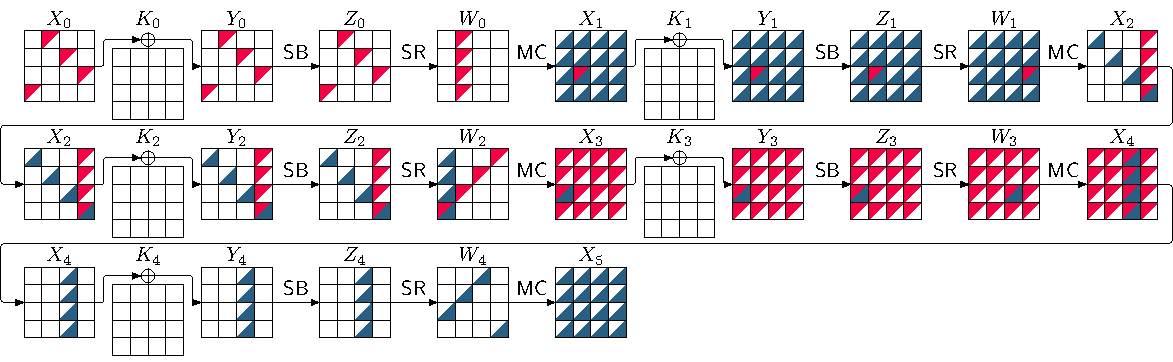
\includegraphics[width=\textwidth]{./figures/aes_sk_5r_v0.pdf} % Replace with your third shape
\end{center}
\begin{center}
  \resizebox{0.9\textwidth}{!}{
\begin{tabular}{@{}cc@{}}
  \toprule
  \multicolumn{2}{c}{$r_{0} = 1, r_{m} = 3, r_{1} = 1, ~ p = 2^{-24.00}, r = 2^{-7.66}, ~ q^{2} = 2^{-24.00}, ~ prq^{2} = 2^{-55.66}$}\\
  \midrule
  $\Delta X_{0}$ \small\texttt{001c00000000e200000000dfb3000000} & $\Delta X_{1}$ \small\texttt{000000000000000000f7000000000000}\\
  $\Gamma X_{4}$ \small\texttt{00000000000000006700000000000000} & $\Gamma X_{5}$ \small\texttt{21d3814d93b1ef228e923507f67383fd}\\
  \bottomrule
\end{tabular}}
\end{center}
\end{frame}

%%%%%%%%%%%%%%%%%%%%%%%%%%%%%%%%%%%%%%%%%%%%%%%%%%%%%%%%%%%%%%%%%%%%%%%%
\begin{frame}{Example: Distinguishers for up to 17 Rounds of \cipher{TWINE}}
\begin{itemize}
  \item Comparing the data complexity of best boomerang and DL distinguishers
\end{itemize}
\begin{center}
\begin{tabular}[t]{c|c|c|c}
\toprule
\# Rounds    &  Boomerang \cite{tosc_HadipourNE22} & Differential-Linear & Gain\\
\midrule
5            &  1            & 1           & 1\\
7            &  $2^{3.20}$   & 1           & $2^{3.20}$\\
13           &  $2^{34.32}$  & $2^{27.16}$ & $2^{7.16}$\\
14           &  $2^{42.25}$  & $2^{31.28}$ & $2^{10.97}$\\
15           &  $2^{51.03}$  & $2^{38.98}$ & $2^{12.05}$\\
16           &  $2^{58.04}$  & $2^{47.28}$ & $2^{10.76}$\\
\textbf{17}  &  -            & $2^{59.24}$ & - \\
\bottomrule
\end{tabular}
\end{center}
\end{frame}

%%%%%%%%%%%%%%%%%%%%%%%%%%%%%%%%%%%%%%%%%%%%%%%%%%%%%%%%%%%%%%%%%%%%%%%%
\begin{frame}{Example: Distinguishers for up to 17 Rounds of \cipher{LBlock}}
\begin{itemize}
  \item Comparing the data complexity of best boomerang and DL distinguishers
\end{itemize}
\begin{center}
\begin{tabular}[t]{c|c|c|c}
\toprule
\# Rounds    &  Boomerang \cite{tosc_HadipourNE22} & Differential-Linear & Gain\\
\midrule
5            &  1            & 1           & 1\\
7            &  $2^{2.97}$   & 1           & $2^{2.97}$\\
13           &  $2^{30.28}$  & $2^{23.78}$ & $2^{6.50}$\\
14           &  $2^{38.86}$  & $2^{30.34}$ & $2^{8.52}$\\
15           &  $2^{46.90}$  & $2^{38.26}$ & $2^{8.64}$\\
16           &  $2^{57.16}$  & $2^{46.26}$ & $2^{10.90}$\\
\textbf{17}  &  -            & $2^{58.30}$ & - \\
\bottomrule
\end{tabular}
\end{center}
\end{frame}

%%%%%%%%%%%%%%%%%%%%%%%%%%%%%%%%%%%%%%%%%%%%%%%%%%%%%%%%%%%%%%%%%%%%%%%%
\begin{frame}{Example: Distinguishers for up to 8 Rounds of \cipher{CLEFIA}}
\begin{itemize}
  \item Comparing the data complexity of best boomerang and DL distinguishers
\end{itemize}
\begin{center}
\begin{tabular}[t]{c|c|c|c}
\toprule
\# Rounds    &  Boomerang \cite{tosc_HadipourNE22} & Differential-Linear & Gain\\
\midrule
3            &  1            & 1           & 1\\
4            &  $2^{6.32}$   & 1           & $2^{6.32}$\\
5            &  $2^{12.26}$  & $2^{5.36}$  & $2^{6.90}$\\
6            &  $2^{22.45}$  & $2^{14.14}$ & $2^{8.31}$\\
7            &  $2^{32.67}$  & $2^{23.50}$ & $2^{9.17}$\\
8            &  $2^{76.03}$  & $2^{66.86}$ & $2^{9.17}$\\
\bottomrule
\end{tabular}
\end{center}
\end{frame}

%%%%%%%%%%%%%%%%%%%%%%%%%%%%%%%%%%%%%%%%%%%%%%%%%%%%%%%%%%%%%%%%%%%%%%%%
\begin{frame}{Application to \cipher{Ascon-p}({\tiny\dllegend})}
\vspace{-0.6cm}
\begin{columns}
\column[c]{0.5\textwidth}
\begin{center}
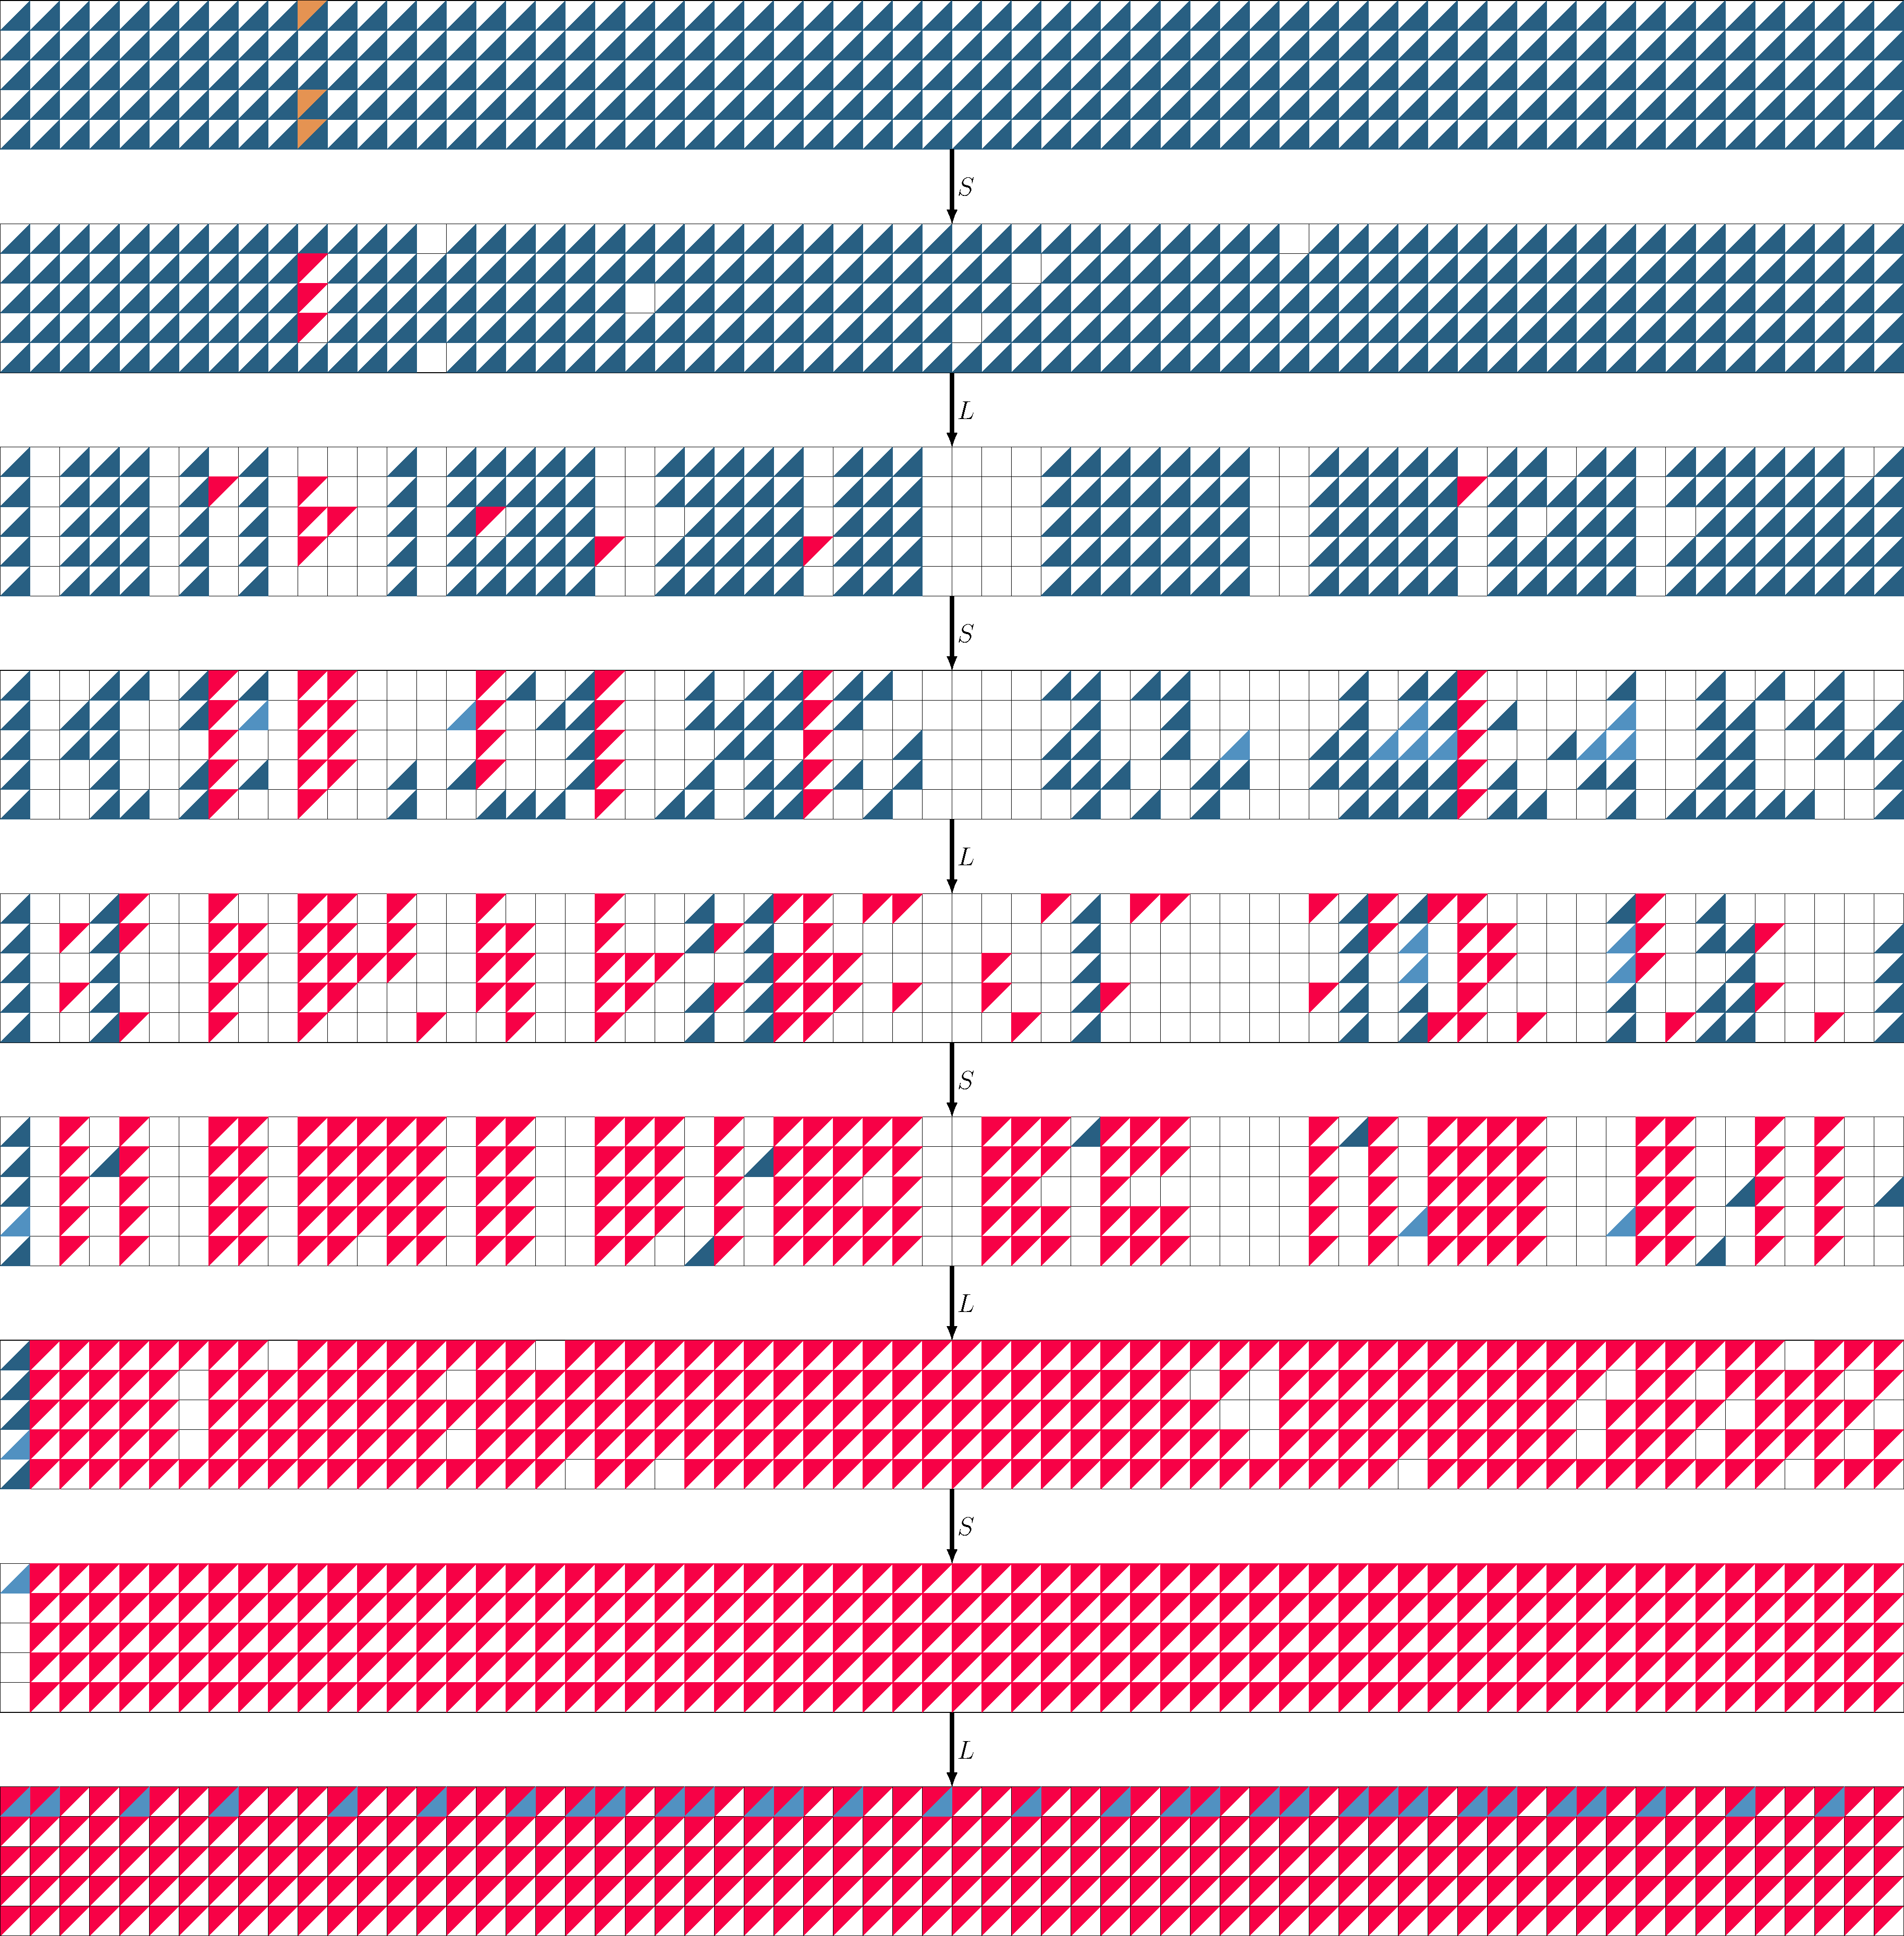
\includegraphics[width=0.75\textwidth]{./figures/ascon_4r_v0.pdf}
\vspace{-0.5cm}
{\scriptsize \[\corr = 1\]}
\end{center}
\column[c]{0.5\textwidth}
\begin{center}
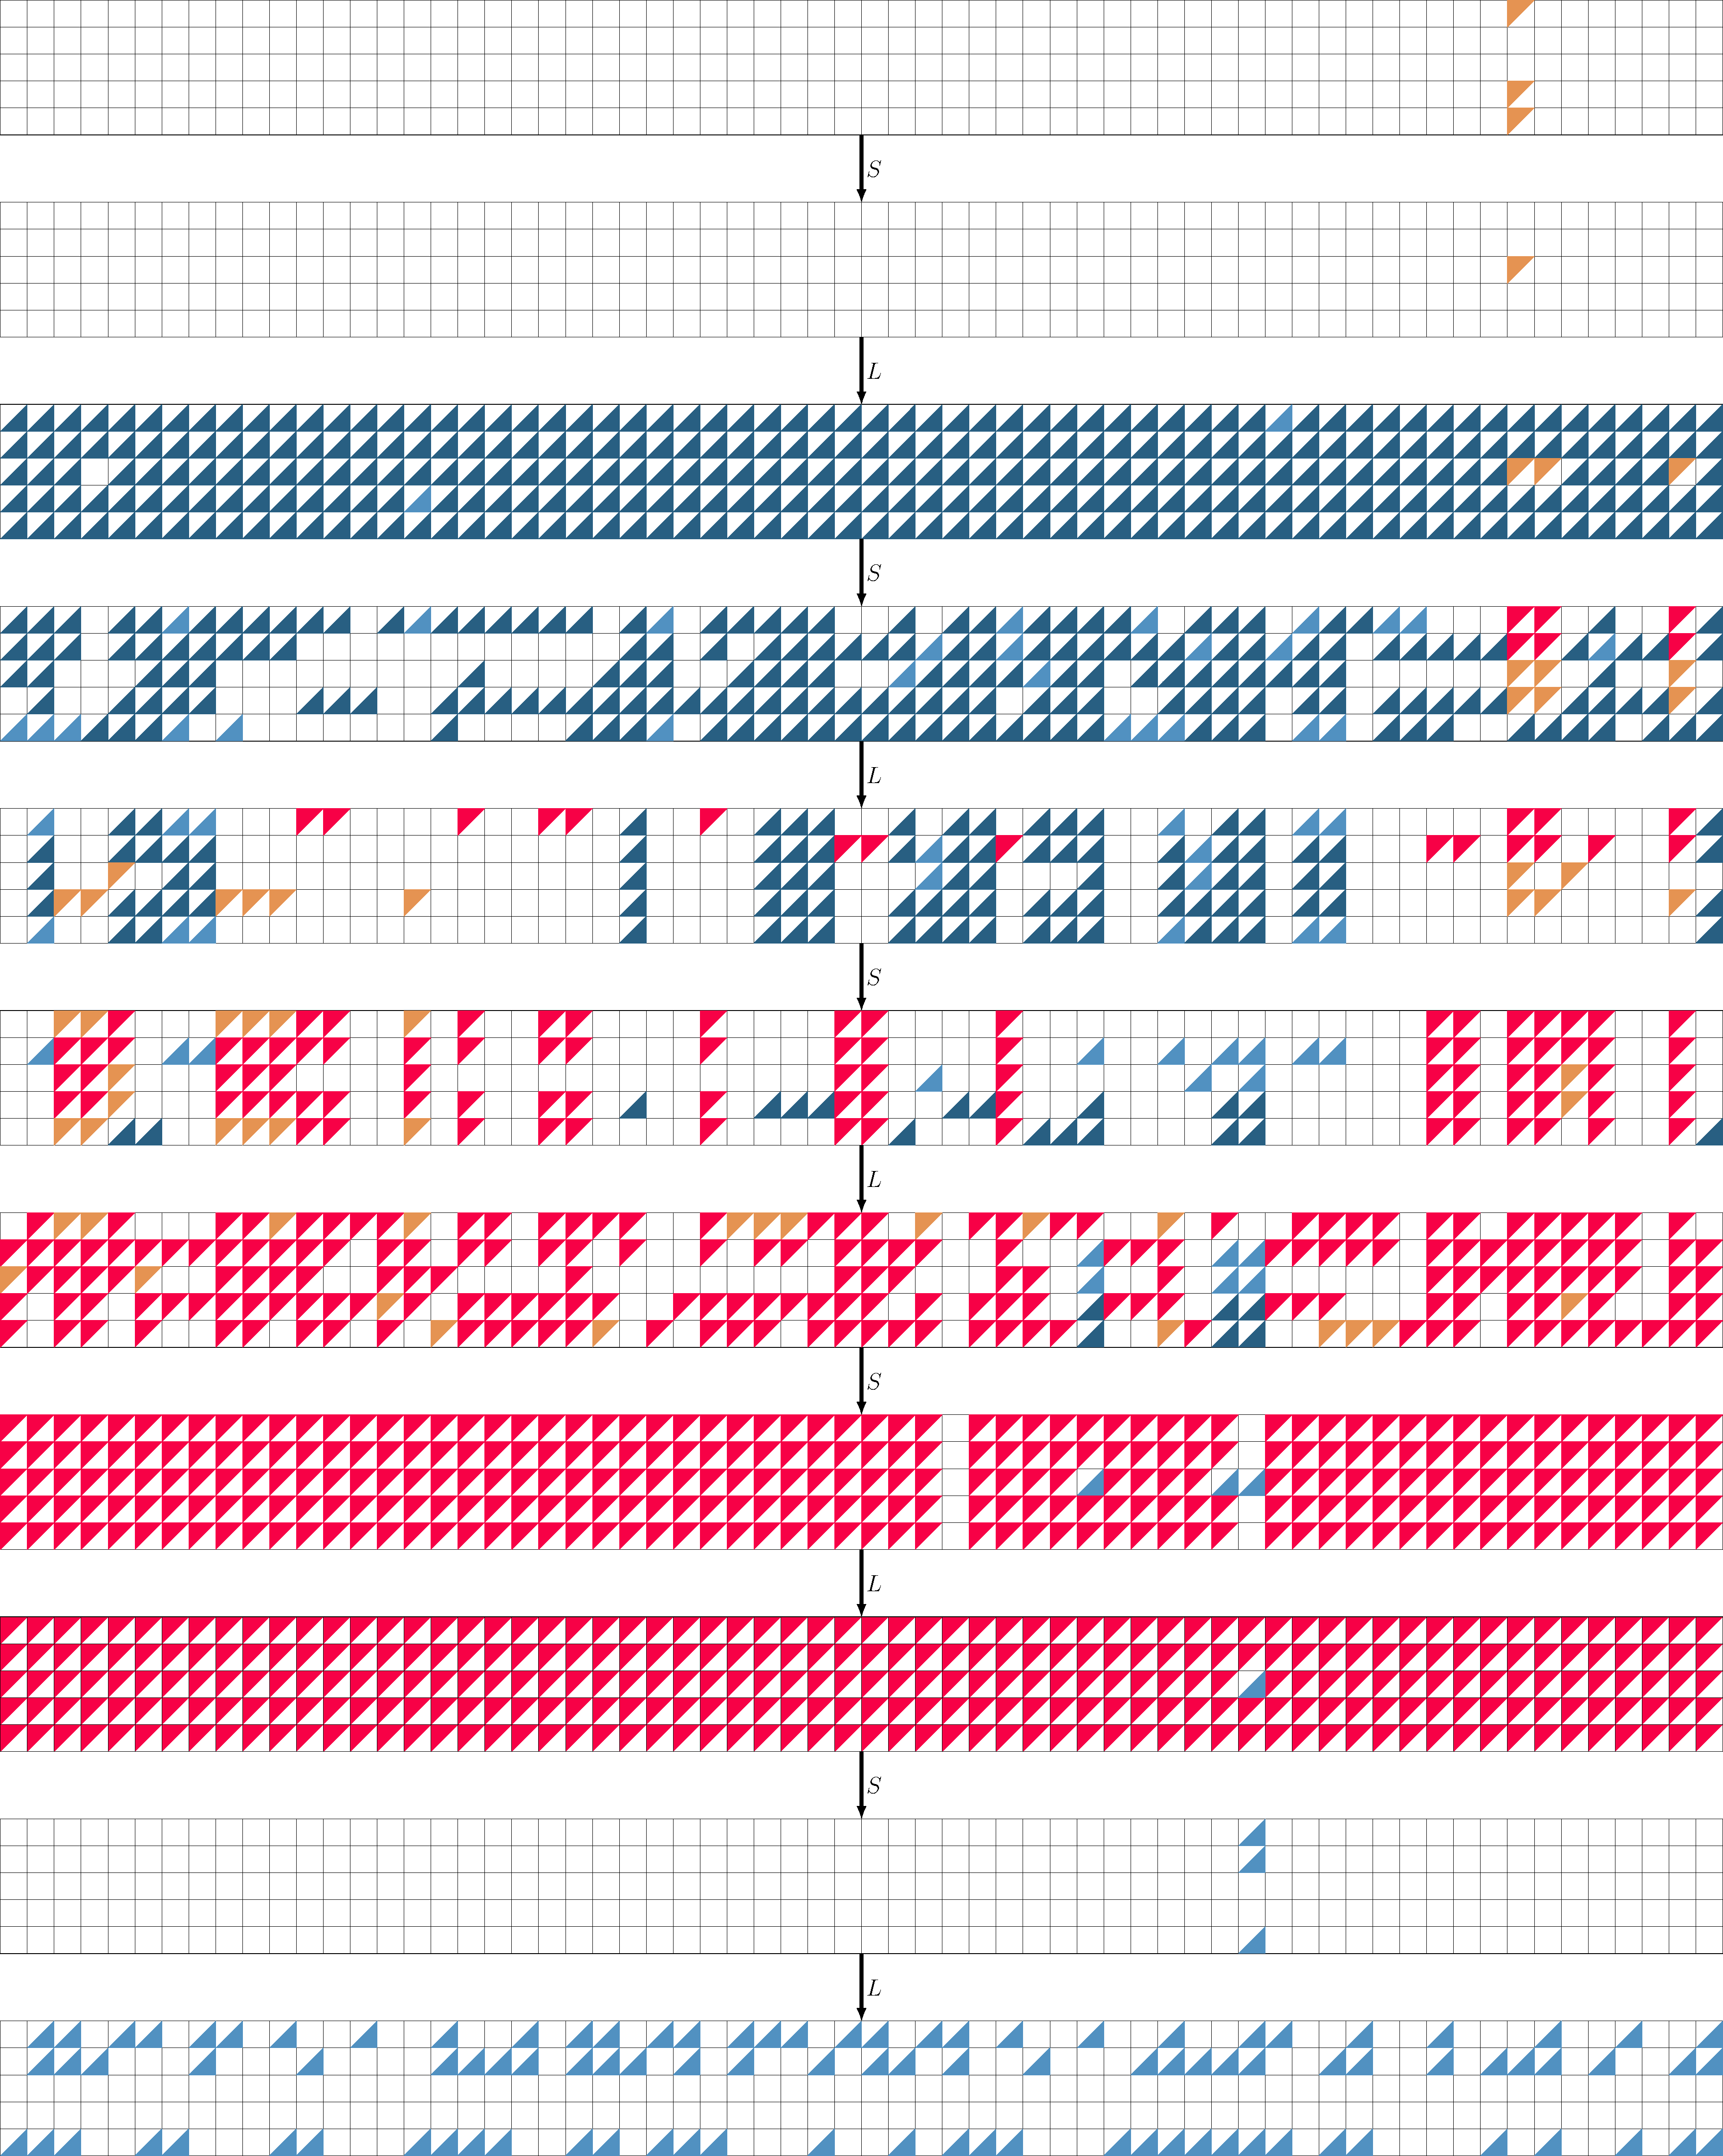
\includegraphics[width=0.68\textwidth]{./figures/ascon_5r_v0.pdf}
\vspace{-0.5cm}
{\scriptsize \[\corr = 2^{-4.33}\]}
\end{center}
\end{columns}
\end{frame}

%%%%%%%%%%%%%%%%%%%%%%%%%%%%%%%%%%%%%%%%%%%%%%%%%%%%%%%%%%%%%%%%%%%%%%%%
\begin{frame}{Application to \cipher{SERPENT}}
\vspace{-0.5cm}
\begin{itemize}
  \item \faLaptop: Experimentally verified
\end{itemize}
\vspace{-0.2cm}
\begin{table}
  \centering
  \newcommand{\ph}{\phantom{.00}}
  \newcommand{\YY}{\checkmark}
  \begin{tabular}[t]{@{}lclcr@{}}
    \toprule
    Cipher                                 & \#R    & $\corr$         & \faLaptop & Ref.\\
    \midrule
    \multirow{8}{*}{\cipher{SERPENT}}
                                            & 3      &  $\bf2^{-0.68}$ & \YY & This work\\
                                            & 4      &    $2^{-12.75}$ &     & \cite{indocrypt_DunkelmanIK08}\\
                                            & 4      &  $\bf2^{-5.54}$ & \YY & This work\\
                                            & 5      &    $2^{-16.75}$ &     & \cite{indocrypt_DunkelmanIK08}\\
                                            & 5      & $\bf2^{-11.10}$ & \YY & This work\\
                                            & 8      &    $2^{-39.18}$ &     & This work\\
                                            & 9      &    $2^{-56.50}$ &     & \cite{indocrypt_DunkelmanIK08}\\
                                            & 9      & $\bf2^{-50.95}$ &     & This work\\
    \bottomrule
  \end{tabular}
\end{table}
\end{frame}

%%%%%%%%%%%%%%%%%%%%%%%%%%%%%%%%%%%%%%%%%%%%%%%%%%%%%%%%%%%%%%%%%%%%%%%%
\begin{frame}{Application to \cipher{Simeck}}
\sparen
\begin{itemize}
  \item \faLaptop: Experimentally verified
\end{itemize}
\sparen
\begin{columns}
\newcommand{\ph}{\phantom{.00}}
\newcommand{\YY}{\checkmark}
\column[c]{0.33\textwidth}
\begin{center}
\resizebox{0.97\textwidth}{!}{
\begin{tabular}[t]{@{}lclcr@{}}
  % TODO maybe select 1 more line to show
  \toprule
  Cipher                                 & \#R    & $\corr$         & \faLaptop & Ref.\\
  \midrule
  \multirow{3}{*}{\cipher{Simeck}-32}
                                          & 7      &  $\bf1$         & \YY & This work\\                                           
                                          & 14     &    $2^{-16.63}$ &     & \cite{zhou2024milp}\\
                                          & 14     & $\bf2^{-13.92}$ & \YY & This work\\
  \bottomrule
\end{tabular}
}
\end{center}

\column[c]{0.33\textwidth}
\begin{center}
\resizebox{0.97\textwidth}{!}{
\begin{tabular}[t]{@{}lclcr@{}}
  % TODO maybe select 1 more line to show
  \toprule
  Cipher                                 & \#R    & $\corr$         & \faLaptop & Ref.\\
  \midrule
  \multirow{7}{*}{\cipher{Simeck}-48}
                                          & 8      &  $\bf1$         & \YY & This work\\
                                          & 17     &    $2^{-22.37}$ &     & \cite{zhou2024milp}\\
                                          & 17     & $\bf2^{-13.89}$ & \YY & This work\\
                                          & 18     &    $2^{-24.75}$ &     & \cite{zhou2024milp}\\
                                          & 18     & $\bf2^{-15.89}$ &     & This work\\
                                          & \bf19  & $\bf2^{-17.89}$ &     & This work\\
                                          & \bf20  & $\bf2^{-21.89}$ &     & This work\\
  \bottomrule
\end{tabular}
}
\end{center}
\column[c]{0.33\textwidth}
\begin{center}
\resizebox{0.97\textwidth}{!}{
\begin{tabular}[t]{@{}lclcr@{}}
  % TODO maybe select 1 more line to show
  \toprule
  Cipher                                 & \#R    & $\corr$         & \faLaptop & Ref.\\
  \midrule
  \multirow{6}{*}{\cipher{Simeck}-64}
                                          & 10     &  $\bf1$         & \YY & This work\\
                                          & 24     &    $2^{-38.13}$ &     & \cite{zhou2024milp}\\
                                          & 24     & $\bf2^{-25.14}$ &     & This work\\
                                          & 25     &    $2^{-41.04}$ &     & \cite{zhou2024milp}\\
                                          & 25     & $\bf2^{-27.14}$ &     & This work\\
                                          & \bf26  & $\bf2^{-30.35}$ &     & This work\\
  \bottomrule
\end{tabular}
}
\end{center}
\end{columns}
\end{frame}

%%%%%%%%%%%%%%%%%%%%%%%%%%%%%%%%%%%%%%%%%%%%%%%%%%%%%%%%%%%%%%%%%%%%%%%%
%%%%%%%%%%%%%%%%%%%%%%%%%%%%%%%%%%%%%%%%%%%%%%%%%%%%%%%%%%%%%%%%%%%%%%%%
\section{Contributions and Future Works}
\sectionheader[\huge\color{tug}\faHourglassEnd]{Contributions and Future Works}

\begin{frame}{Contributions and Future Works}
\vspace{-0.5cm}
\begin{itemize}
\item Contributions
\begin{itemize}
\small
\item[\textcolor{tugred}{\faDiamond}] We generalized the \dlct framework from one S-box layer to multiple rounds
\item[\textcolor{tugred}{\faDiamond}] We proposed an automatic tool for finding optimum DL distinguishers
\item[\textcolor{tugred}{\faDiamond}] We applied our tool to almost any design paradigm
\end{itemize}
\item Future works
\begin{itemize}
\small
\item[\faRoad] Extedning the application of our tool to other primitives, e.g., ARX 
\item[\faRoad] Extending our tool to a unified model for finding complete attack (key recovery)
% \item[\faRoad] Exploiting neutral bits when searching for distinguishers
\end{itemize} 
\end{itemize}
\begin{center}
\vspace{0.10cm}

% {\large Thanks for your attention!}

% \vspace{0.3cm}
% \faGithub: \url{https://github.com/hadipourh/zero}\\
\vspace{0.1cm}
\faArchive: \url{https://ia.cr/2024/255}
\end{center}
\end{frame}

















%%%%%%%%%%%%%%%%%%%%%%%%%%%%%%%%%%%%%%%%%%%%%%%%%%%%%%%%%%%%%%%%%%%%%%%%%%%%

\begin{frame}[allowframebreaks]{Bibliography}
  \printbibliography
\end{frame}

%%%%%%%%%%%%%%%%%%%%%%%%%%%%%%%%%%%%%%%%%%%%%%%%%%%%%%%%%%%%%%%%%%%%%%%%%%%%


%%%%%%%%%%%%%%%%%%%%%%%%%%%%%%%%%%%%%%%%%%%%%%%%%%%%%%%%%%%%%%%%%%%%%%%%%%%%
% Bakcup slides

\begin{frame}{Properties of Generalized \dlct Tables - I}
\begin{itemize}
  \item $\dlct(\Delta\In, \lambda\Out) = \sum_{\Delta\Out} \udlct(\Delta\In, \Delta\Out, \lambda\Out) $ %, $\forall \Delta\In, \lambda\Out$
  \item $\udlct(\Delta\In, \Delta\Out, \lambda\Out) = (-1)^{\Delta\Out \cdot \lambda\Out} \ddt(\Delta\In, \Delta\Out)$
  \item $\ldlct(\Delta\In, \lambda\In, \lambda\Out) = (-1)^{\Delta\In \cdot \lambda\In} \dlct(\Delta\In, \lambda\Out)$
  \item $\edlct(\Delta\In, \Delta\Out, \lambda\In, \lambda\Out) = (-1)^{\lambda\In \cdot \Delta\In \oplus \lambda\Out \cdot \Delta\Out} \ddt(\Delta\In, \Delta\Out)$
  \item $\ldlct(\Delta\In, \lambda\In, \lambda\Out) = \sum_{\Delta\Out} \edlct(\Delta\In, \Delta\Out, \lambda\In, \lambda\Out)$ %,  $\forall \Delta\In, \lambda\In, \lambda\Out$
  \item $\sum_{\Delta\In} \ldlct(\Delta\In, \lambda\In, \lambda\Out) = \lat^{2}(\lambda\In, \lambda\Out)$
\end{itemize}
\end{frame}

\begin{frame}{Properties of Generalized \dlct Tables - II}
\begin{itemize}
\item $\ddlct(\Delta\In, \lambda\Out) = 2^{-n}\cdot\sum_{\Delta\Mid}\sum_{\lambda\Mid}  \udlct\left(\Delta\In, \Delta\Mid, \lambda\Mid\right) \cdot \ldlct\left(\Delta\Mid, \lambda\Mid, \lambda\Out\right)$
\end{itemize}
\begin{align*}
\ddlct(\Delta\In, \lambda\Out) &= \sum_{\Delta\Mid} \ddt(\Delta\In, \Delta\Mid) \cdot \dlct(\Delta\Mid, \lambda\Out)\\
                        &= 2^{-n}\sum_{\lambda\Mid} \dlct(\Delta\In, \lambda\Mid)\cdot\lat^{2}(\lambda\Mid, \lambda\Out).
                      % &= \sum_{\Delta\Mid}\sum_{\lambda\Mid}  \udlct\left(\Delta\In, \Delta\Mid, \lambda\Mid\right) \ldlct\left(\Delta\Mid, \lambda\Mid, \lambda\Out\right)
\end{align*}
\end{frame}
%%%%%%%%%%%%%%%%%%%%%%%%%%%%%%%%%%%%%%%%%%%%%%%%%%%%%%%%%%%%%%%%%%%%%%%%%%%%
%%%%%%%%%%%%%%%%%%%%%%%%%%%%%%%%%%%%%%%%%%%%%%%%%%%%%%%%%%%%%%%%%%%%%%%%%%%%

\begin{filecontents*}[overwrite]{\jobname.bib}

% Seminal paper of Differential-Linear Cryptanalysis
@inproceedings{dl_crypto_LangfordH94,
  author       = {Susan K. Langford and
                  Martin E. Hellman},
  title        = {Differential-Linear Cryptanalysis},
  booktitle    = {{CRYPTO} '94},
  volume       = {839},
  pages        = {17--25},
  publisher    = {Springer},
  year         = {1994},
  doi          = {10.1007/3-540-48658-5_3}
}

% AES specification
@article{daemen1999aes,
  title={AES proposal: Rijndael},
  author={Daemen, Joan and Rijmen, Vincent},
  year={1999},
  publisher={Gaithersburg, MD, USA}
}

% seminal paper for differential cryptanalysis
@inproceedings{crypto_BihamS90,
  author       = {Eli Biham and
                  Adi Shamir},
  editor       = {Alfred Menezes and
                  Scott A. Vanstone},
  title        = {Differential Cryptanalysis of {DES}-like Cryptosystems},
  booktitle    = {{CRYPTO} '90},
  series       = {LNCS},
  volume       = {537},
  pages        = {2--21},
  publisher    = {Springer},
  year         = {1990},
  doi          = {10.1007/3-540-38424-3_1}
}

% seminal paper for linear cryptanalysis (Piling-up lemma)
@inproceedings{eurocrypt_Matsui93,
  author       = {Mitsuru Matsui},
  editor       = {Tor Helleseth},
  title        = {Linear Cryptanalysis Method for {DES} Cipher},
  booktitle    = {{EUROCRYPT} '93},
  series       = {LNCS},
  volume       = {765},
  pages        = {386--397},
  publisher    = {Springer},
  year         = {1993},
  doi          = {10.1007/3-540-48285-7_33}
}

% Formalizes the complexity of DL attacks
@article{journals_joc_BlondeauLN17,
  author       = {C{\'{e}}line Blondeau and
                  Gregor Leander and
                  Kaisa Nyberg},
  title        = {Differential-Linear Cryptanalysis Revisited},
  journal      = {J. Cryptol.},
  volume       = {30},
  number       = {3},
  pages        = {859--888},
  year         = {2017},
  doi          = {10.1007/s00145-016-9237-5}
}

% sandwich framework
@article{joc_DunkelmanKS14,
  author       = {Orr Dunkelman and
                  Nathan Keller and
                  Adi Shamir},
  title        = {A Practical-Time Related-Key Attack on the {KASUMI} Cryptosystem Used
                  in {GSM} and {3G} Telephony},
  journal      = {J. Cryptol.},
  volume       = {27},
  number       = {4},
  pages        = {824--849},
  year         = {2014},
  doi          = {10.1007/s00145-013-9154-9}
}

% DLCT paper. This is also the first paper splitting the cipher into three parts for DL analysis.
@inproceedings{dlct_eurocrypt_BarOnDKW19,
  author       = {Achiya Bar{-}On and
                  Orr Dunkelman and
                  Nathan Keller and
                  Ariel Weizman},
  title        = {{DLCT:} {A} New Tool for Differential-Linear Cryptanalysis},
  booktitle    = {{EUROCRYPT} 2019},
  series       = {LNCS},
  volume       = {11476},
  pages        = {313--342},
  publisher    = {Springer},
  year         = {2019},
  doi          = {10.1007/978-3-030-17653-2_11}
}

@inproceedings{fse_Wagner99,
  author    = {David A. Wagner},
  title     = {The Boomerang Attack},
  booktitle = {{FSE}},
  series    = {LNCS},
  volume    = {1636},
  pages     = {156--170},
  publisher = {Springer},
  doi       = {10.1007/3-540-48519-8_12},
  year      = {1999}
}

@inproceedings{fse_BlondeauLN14,
  author       = {C{\'{e}}line Blondeau and
                  Gregor Leander and
                  Kaisa Nyberg},
  editor       = {Carlos Cid and
                  Christian Rechberger},
  title        = {Differential-Linear Cryptanalysis Revisited},
  booktitle    = {{FSE} 2014},
  series       = {LNCS},
  volume       = {8540},
  pages        = {411--430},
  publisher    = {Springer},
  year         = {2014},
  doi          = {10.1007/978-3-662-46706-0_21},
}

@inproceedings{conf_crypto_DunkelmanKS10,
	author    = {Orr Dunkelman and
		         Nathan Keller and
		         Adi Shamir},
	title     = {A Practical-Time Related-Key Attack on the {KASUMI} Cryptosystem Used
		in {GSM} and 3G Telephony},
	booktitle = {{CRYPTO}},
	series    = {LNCS},
	volume    = {6223},
	pages     = {393--410},
	publisher = {Springer},
	doi       = {10.1007/978-3-642-14623-7_21},
	year      = {2010}
}

@inproceedings{eurocrypt_CidHPSS18,
  author       = {Carlos Cid and
                  Tao Huang and
                  Thomas Peyrin and
                  Yu Sasaki and
                  Ling Song},
  editor       = {Jesper Buus Nielsen and
                  Vincent Rijmen},
  title        = {Boomerang Connectivity Table: {A} New Cryptanalysis Tool},
  booktitle    = {{EUROCRYPT} 2018},
  series       = {LNCS},
  volume       = {10821},
  pages        = {683--714},
  publisher    = {Springer},
  year         = {2018},
  doi          = {10.1007/978-3-319-78375-8_22}
}

@article{tosc_WangP19,
  author       = {Haoyang Wang and
                  Thomas Peyrin},
  title        = {Boomerang Switch in Multiple Rounds. Application to {AES} Variants
                  and Deoxys},
  journal      = {{IACR} Trans. Symmetric Cryptol.},
  volume       = {2019},
  number       = {1},
  pages        = {142--169},
  year         = {2019},
  doi          = {10.13154/TOSC.V2019.I1.142-169}
}

@article{tosc_DelauneDV20,
  author       = {St{\'{e}}phanie Delaune and
                  Patrick Derbez and
                  Mathieu Vavrille},
  title        = {Catching the Fastest Boomerangs Application to {SKINNY}},
  journal      = {{IACR} Trans. Symmetric Cryptol.},
  volume       = {2020},
  number       = {4},
  pages        = {104--129},
  year         = {2020},
  doi          = {10.46586/TOSC.V2020.I4.104-129}
}

@article{tosc_SongQH19,
  author       = {Ling Song and
                  Xianrui Qin and
                  Lei Hu},
  title        = {Boomerang Connectivity Table Revisited. Application to {SKINNY} and
                  {AES}},
  journal      = {{IACR} Trans. Symmetric Cryptol.},
  volume       = {2019},
  number       = {1},
  pages        = {118--141},
  year         = {2019},
  url          = {https://doi.org/10.13154/tosc.v2019.i1.118-141},
  doi          = {10.13154/TOSC.V2019.I1.118-141},
}

@article{tosc_BoukerrouHLMM20,
  author       = {Hamid Boukerrou and
                  Paul Huynh and
                  Virginie Lallemand and
                  Bimal Mandal and
                  Marine Minier},
  title        = {On the Feistel Counterpart of the Boomerang Connectivity Table Introduction
                  and Analysis of the {FBCT}},
  journal      = {{IACR} Trans. Symmetric Cryptol.},
  volume       = {2020},
  number       = {1},
  pages        = {331--362},
  year         = {2020},
  doi          = {10.13154/TOSC.V2020.I1.331-362},
}

@article{tosc_HadipourBS21,
  author       = {Hosein Hadipour and
                  Nasour Bagheri},
  title        = {Improved Rectangle Attacks on {SKINNY} and {CRAFT}},
  journal      = {{IACR} Trans. Symmetric Cryptol.},
  volume       = {2021},
  number       = {2},
  pages        = {140--198},
  year         = {2021},
  doi          = {10.46586/TOSC.V2021.I2.140-198},
}

@article{tosc_HadipourNE22,
  author       = {Hosein Hadipour and
                  Marcel Nageler and
                  Maria Eichlseder},
  title        = {Throwing Boomerangs into Feistel Structures Application to CLEFIA,
                  WARP, LBlock, LBlock-s and {TWINE}},
  journal      = {{IACR} Trans. Symmetric Cryptol.},
  volume       = {2022},
  number       = {3},
  pages        = {271--302},
  year         = {2022},
  doi          = {10.46586/TOSC.V2022.I3.271-302},
}

% more precise measurement of bias for 9-round DL distinguisher of serpent
@inproceedings{indocrypt_DunkelmanIK08,
  author       = {Orr Dunkelman and
                  Sebastiaan Indesteege and
                  Nathan Keller},
  editor       = {Dipanwita Roy Chowdhury and
                  Vincent Rijmen and
                  Abhijit Das},
  title        = {A Differential-Linear Attack on 12-Round {Serpent}},
  booktitle    = {{INDOCRYPT} 2008},
  series       = {LNCS},
  volume       = {5365},
  pages        = {308--321},
  publisher    = {Springer},
  year         = {2008},
  doi          = {10.1007/978-3-540-89754-5_24}
}

% application of miqcp to simeck
@article{zhou2024milp,
  title        = {{MILP/MIQCP}-Based Fully Automatic Method of Searching for Differential-Linear Distinguishers for {SIMON}-Like Ciphers},
  author       = {Zhou, Yanyan and  
                  Wang, Senpeng and 
                  Hu, Bin},
  journal      = {IET Information Security},
  volume       = {2024},
  year         = {2024},
  publisher    = {Hindawi},
  doi          = {10.1049/2024/8315115}
}

\end{filecontents*}

\end{document}
